% Options for packages loaded elsewhere
\PassOptionsToPackage{unicode}{hyperref}
\PassOptionsToPackage{hyphens}{url}
%
\documentclass[
]{book}
\usepackage{lmodern}
\usepackage{amssymb,amsmath}
\usepackage{ifxetex,ifluatex}
\ifnum 0\ifxetex 1\fi\ifluatex 1\fi=0 % if pdftex
  \usepackage[T1]{fontenc}
  \usepackage[utf8]{inputenc}
  \usepackage{textcomp} % provide euro and other symbols
\else % if luatex or xetex
  \usepackage{unicode-math}
  \defaultfontfeatures{Scale=MatchLowercase}
  \defaultfontfeatures[\rmfamily]{Ligatures=TeX,Scale=1}
\fi
% Use upquote if available, for straight quotes in verbatim environments
\IfFileExists{upquote.sty}{\usepackage{upquote}}{}
\IfFileExists{microtype.sty}{% use microtype if available
  \usepackage[]{microtype}
  \UseMicrotypeSet[protrusion]{basicmath} % disable protrusion for tt fonts
}{}
\makeatletter
\@ifundefined{KOMAClassName}{% if non-KOMA class
  \IfFileExists{parskip.sty}{%
    \usepackage{parskip}
  }{% else
    \setlength{\parindent}{0pt}
    \setlength{\parskip}{6pt plus 2pt minus 1pt}}
}{% if KOMA class
  \KOMAoptions{parskip=half}}
\makeatother
\usepackage{xcolor}
\IfFileExists{xurl.sty}{\usepackage{xurl}}{} % add URL line breaks if available
\IfFileExists{bookmark.sty}{\usepackage{bookmark}}{\usepackage{hyperref}}
\hypersetup{
  pdftitle={A Tour of Machine Learning Tools},
  pdfauthor={Dan MacLean},
  hidelinks,
  pdfcreator={LaTeX via pandoc}}
\urlstyle{same} % disable monospaced font for URLs
\usepackage{color}
\usepackage{fancyvrb}
\newcommand{\VerbBar}{|}
\newcommand{\VERB}{\Verb[commandchars=\\\{\}]}
\DefineVerbatimEnvironment{Highlighting}{Verbatim}{commandchars=\\\{\}}
% Add ',fontsize=\small' for more characters per line
\usepackage{framed}
\definecolor{shadecolor}{RGB}{248,248,248}
\newenvironment{Shaded}{\begin{snugshade}}{\end{snugshade}}
\newcommand{\AlertTok}[1]{\textcolor[rgb]{0.94,0.16,0.16}{#1}}
\newcommand{\AnnotationTok}[1]{\textcolor[rgb]{0.56,0.35,0.01}{\textbf{\textit{#1}}}}
\newcommand{\AttributeTok}[1]{\textcolor[rgb]{0.77,0.63,0.00}{#1}}
\newcommand{\BaseNTok}[1]{\textcolor[rgb]{0.00,0.00,0.81}{#1}}
\newcommand{\BuiltInTok}[1]{#1}
\newcommand{\CharTok}[1]{\textcolor[rgb]{0.31,0.60,0.02}{#1}}
\newcommand{\CommentTok}[1]{\textcolor[rgb]{0.56,0.35,0.01}{\textit{#1}}}
\newcommand{\CommentVarTok}[1]{\textcolor[rgb]{0.56,0.35,0.01}{\textbf{\textit{#1}}}}
\newcommand{\ConstantTok}[1]{\textcolor[rgb]{0.00,0.00,0.00}{#1}}
\newcommand{\ControlFlowTok}[1]{\textcolor[rgb]{0.13,0.29,0.53}{\textbf{#1}}}
\newcommand{\DataTypeTok}[1]{\textcolor[rgb]{0.13,0.29,0.53}{#1}}
\newcommand{\DecValTok}[1]{\textcolor[rgb]{0.00,0.00,0.81}{#1}}
\newcommand{\DocumentationTok}[1]{\textcolor[rgb]{0.56,0.35,0.01}{\textbf{\textit{#1}}}}
\newcommand{\ErrorTok}[1]{\textcolor[rgb]{0.64,0.00,0.00}{\textbf{#1}}}
\newcommand{\ExtensionTok}[1]{#1}
\newcommand{\FloatTok}[1]{\textcolor[rgb]{0.00,0.00,0.81}{#1}}
\newcommand{\FunctionTok}[1]{\textcolor[rgb]{0.00,0.00,0.00}{#1}}
\newcommand{\ImportTok}[1]{#1}
\newcommand{\InformationTok}[1]{\textcolor[rgb]{0.56,0.35,0.01}{\textbf{\textit{#1}}}}
\newcommand{\KeywordTok}[1]{\textcolor[rgb]{0.13,0.29,0.53}{\textbf{#1}}}
\newcommand{\NormalTok}[1]{#1}
\newcommand{\OperatorTok}[1]{\textcolor[rgb]{0.81,0.36,0.00}{\textbf{#1}}}
\newcommand{\OtherTok}[1]{\textcolor[rgb]{0.56,0.35,0.01}{#1}}
\newcommand{\PreprocessorTok}[1]{\textcolor[rgb]{0.56,0.35,0.01}{\textit{#1}}}
\newcommand{\RegionMarkerTok}[1]{#1}
\newcommand{\SpecialCharTok}[1]{\textcolor[rgb]{0.00,0.00,0.00}{#1}}
\newcommand{\SpecialStringTok}[1]{\textcolor[rgb]{0.31,0.60,0.02}{#1}}
\newcommand{\StringTok}[1]{\textcolor[rgb]{0.31,0.60,0.02}{#1}}
\newcommand{\VariableTok}[1]{\textcolor[rgb]{0.00,0.00,0.00}{#1}}
\newcommand{\VerbatimStringTok}[1]{\textcolor[rgb]{0.31,0.60,0.02}{#1}}
\newcommand{\WarningTok}[1]{\textcolor[rgb]{0.56,0.35,0.01}{\textbf{\textit{#1}}}}
\usepackage{longtable,booktabs}
% Correct order of tables after \paragraph or \subparagraph
\usepackage{etoolbox}
\makeatletter
\patchcmd\longtable{\par}{\if@noskipsec\mbox{}\fi\par}{}{}
\makeatother
% Allow footnotes in longtable head/foot
\IfFileExists{footnotehyper.sty}{\usepackage{footnotehyper}}{\usepackage{footnote}}
\makesavenoteenv{longtable}
\usepackage{graphicx,grffile}
\makeatletter
\def\maxwidth{\ifdim\Gin@nat@width>\linewidth\linewidth\else\Gin@nat@width\fi}
\def\maxheight{\ifdim\Gin@nat@height>\textheight\textheight\else\Gin@nat@height\fi}
\makeatother
% Scale images if necessary, so that they will not overflow the page
% margins by default, and it is still possible to overwrite the defaults
% using explicit options in \includegraphics[width, height, ...]{}
\setkeys{Gin}{width=\maxwidth,height=\maxheight,keepaspectratio}
% Set default figure placement to htbp
\makeatletter
\def\fps@figure{htbp}
\makeatother
\setlength{\emergencystretch}{3em} % prevent overfull lines
\providecommand{\tightlist}{%
  \setlength{\itemsep}{0pt}\setlength{\parskip}{0pt}}
\setcounter{secnumdepth}{5}
\usepackage{booktabs}
\usepackage{amsthm}
\makeatletter
\def\thm@space@setup{%
  \thm@preskip=8pt plus 2pt minus 4pt
  \thm@postskip=\thm@preskip
}
\makeatother
\setmainfont[UprightFeatures={SmallCapsFont=AlegreyaSC-Regular}]{Alegreya}
\renewcommand{\textfraction}{0.05}
\renewcommand{\topfraction}{0.8}
\renewcommand{\bottomfraction}{0.8}
\renewcommand{\floatpagefraction}{0.75}
\let\oldhref\href
\renewcommand{\href}[2]{#2\footnote{\url{#1}}}
\usepackage[skins]{tcolorbox}
\newenvironment{task}
{ \begin{tcolorbox}[title=For you to do,title filled] }
{  \end{tcolorbox} }

\newenvironment{reader}
{ \begin{tcolorbox}[colbacktitle=red!50!white,
title=huh?,coltitle=white,
fonttitle=\bfseries] }
{  \end{tcolorbox} }

% \newenvironment{roundup}
% { \begin{tcolorbox}[colbacktitle=yellow!50!white,title=Round Up,title filled] }
%{  \end{tcolorbox} }

\newenvironment{myquote}
{\begin{large}
\begin{itshape}
\begin{minipage}{6cm}
}
{
\begin{vspace}{15mm}
\end{vspace}
\end{minipage}
\end{itshape}
\end{large}
}

\newenvironment{sidenote}
{ \begin{tcolorbox}[colbacktitle=blue!50!white,
title=huh?,coltitle=white,
fonttitle=\bfseries] }
{  \end{tcolorbox} }

\newenvironment{roundup}
{ \begin{tcolorbox}[colbacktitle=yellow!50!white,
title=Round Up,coltitle=black,
fonttitle=\bfseries] }
{  \end{tcolorbox} }
\usepackage[]{natbib}
\bibliographystyle{apalike}

\title{A Tour of Machine Learning Tools}
\author{Dan MacLean}
\date{2021-04-09}

\begin{document}
\maketitle

{
\setcounter{tocdepth}{1}
\tableofcontents
}
\hypertarget{setting-up}{%
\chapter{Setting up}\label{setting-up}}

The primary purpose of this course is to help you to understand how to use statistical tools for machine Learning that will help with your research. The course will try to introduce you to the capabilities and limitations of some widely used machine learning tools, without leaning heavily on the maths or computer science of these things too much. By the end we hope that you'll have a decent appreciation of what machine learning can do for you, though we don't expect that you'll become expert in any way.

We'll be making use of the R statistical programming environment to do that side of the work. The rest of this chapter will help you get that set up on your own computer.

\hypertarget{prerequisites}{%
\section{Prerequisites}\label{prerequisites}}

\hypertarget{knowledge-prerequisites}{%
\subsection{Knowledge prerequisites}\label{knowledge-prerequisites}}

There are no specific knowledge prerequisites for this book but it will be very helpful if you have read and worked through the \texttt{Data\ Driven\ Visualisation}, \texttt{Data\ Exploration}, \texttt{Intro\ to\ Stats}, \texttt{Estimation\ Statistics} and \texttt{Bayesian\ Inference} books and are familiar with R use.

\hypertarget{software-prerequisites}{%
\subsection{Software prerequisites}\label{software-prerequisites}}

You need to install the following stuff for this book:

\begin{enumerate}
\def\labelenumi{\arabic{enumi}.}
\tightlist
\item
  R
\item
  RStudio
\item
  Some R packages: \texttt{tidyverse}, \texttt{factoextra}, \texttt{patchwork}
\end{enumerate}

\hypertarget{installing-r}{%
\section{Installing R}\label{installing-r}}

Follow this link and install the right version for your operating system \url{https://www.stats.bris.ac.uk/R/}

\hypertarget{installing-rstudio}{%
\section{Installing RStudio}\label{installing-rstudio}}

Follow this link and install the right version for your operating system \url{https://www.rstudio.com/products/rstudio/download/}

\hypertarget{installing-r-packages-in-rstudio}{%
\section{Installing R packages in RStudio}\label{installing-r-packages-in-rstudio}}

\hypertarget{standard-packages}{%
\subsection{Standard packages}\label{standard-packages}}

In the RStudio console, type

\texttt{install.packages(c("tidyverse","factoextra",\ "patchwork",\ "ggdendro",\ "class",\ "caret",\ "e1071","randomForest",\ "neuralnet"))}

\hypertarget{motivation}{%
\chapter{Motivation}\label{motivation}}

\hypertarget{open-the-pod-bay-doors-please-hal.}{%
\section{Open the pod bay doors, please, HAL.}\label{open-the-pod-bay-doors-please-hal.}}

Many of us nowadays own a wide range of genuinely powerful computers. Smart Speakers, Mobile Phones, Gaming Consoles and Laptops and Desktops are extremely capable machines that can run software and algorithms that were in the realms of science fiction not very long ago. The increase in computing power has facilitated an expansion in the class of algorithms known as machine learners. These algorithms are part of the general field of Artificial Intelligence (AI). AI is roughly the ability of machines to make demonstrate intelligence, such as making decisions or learning skills or solving problems for which no explicit protocol is given. We are often introduced to AI by films and science fiction and it is generally seen to be a thing to be feared or exploited.

\begin{figure}
\centering
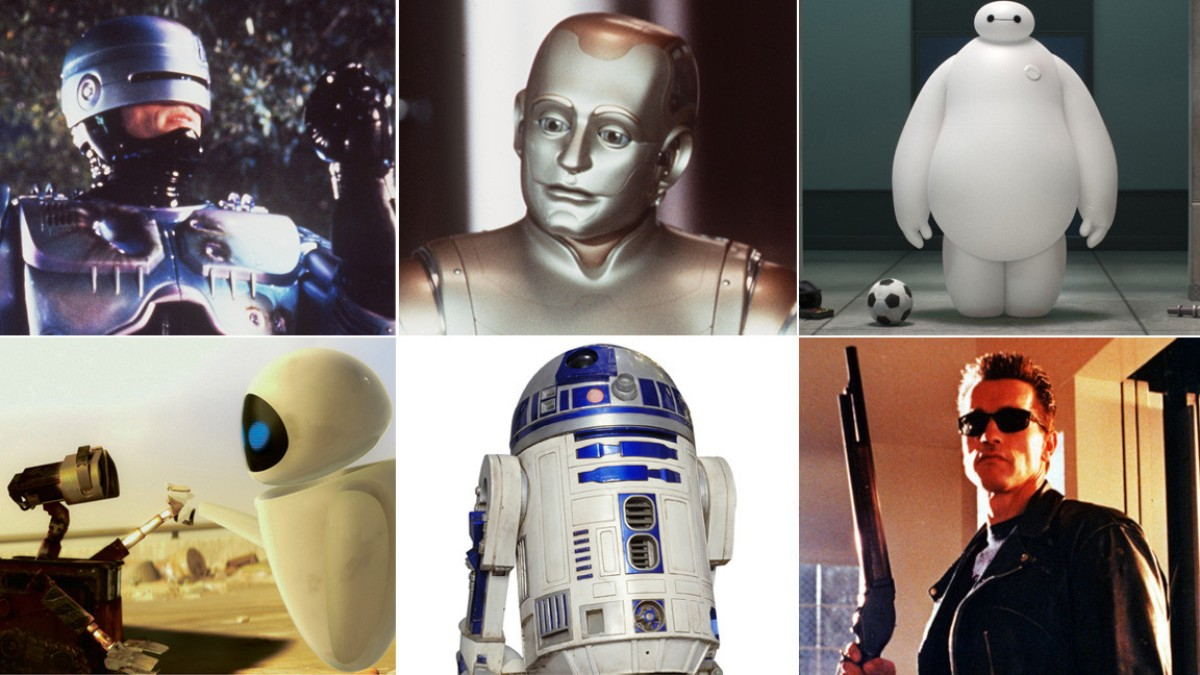
\includegraphics{figs/bots.jpeg}
\caption{\label{fig:unnamed-chunk-2}Some AI, yesterday.}
\end{figure}

But the aspects of AI in machine learning algorithms that we have today are extremely useful in helping us to make sense of data. Because machine learning is concerned with algorithms that improve through experience and by learning from data, they can help us to see patterns and connections in data that we would not be able to see ourselves. Essentially by performing many calculations machine learning algorithms can help us to find structure or divisions in data, perform classifications, create simplifications of complex structures and make data based decisions. These are the algorithms that help us to make sense of the vast swathes of data that we generate in our daily lives and we can make use of them too to help us make sense of complex experimental data.

In this course we'll tour the main classes of machine learning algorithm, with a focus on ones that are common in biological data analysis. This will not be a deep dive, though we will detail the workings of some at a high level. The objective is to tour the galaxy of ML and finish with an appreciation of how they can help and how you can start to make use of such mathematically complex and powerful tools in your research.

\hypertarget{r-fundamentals}{%
\chapter{R Fundamentals}\label{r-fundamentals}}

\hypertarget{about-this-chapter}{%
\section{About this chapter}\label{about-this-chapter}}

\begin{enumerate}
\def\labelenumi{\arabic{enumi}.}
\tightlist
\item
  Questions:
\end{enumerate}

\begin{itemize}
\tightlist
\item
  How do I use R?
\end{itemize}

\begin{enumerate}
\def\labelenumi{\arabic{enumi}.}
\setcounter{enumi}{1}
\tightlist
\item
  Objectives:
\end{enumerate}

\begin{itemize}
\tightlist
\item
  Become familiar with R syntax
\item
  Understand the concepts of objects and assignment
\item
  Get exposed to a few functions
\end{itemize}

\begin{enumerate}
\def\labelenumi{\arabic{enumi}.}
\setcounter{enumi}{2}
\tightlist
\item
  Keypoints:
\end{enumerate}

\begin{itemize}
\tightlist
\item
  R's capabilities are provided by functions
\item
  R users call functions and get results
\end{itemize}

\hypertarget{working-with-r}{%
\section{Working with R}\label{working-with-r}}

In this workshop we'll use R in the extremely useful RStudio software. For the most part we'll work interactively, meaning we'll type stuff straight into the R console in RStudio (Usually this is a window on the left or lower left) and get our results there too (usually in the console or in a window on the right).

Panels like the ones below mimic the interaction with R and first show the thing to type into R, and below the calculated result from R.

Let's look at how R works by using it for it's most basic job - as a calculator:

\begin{Shaded}
\begin{Highlighting}[]
 \DecValTok{3} \OperatorTok{+}\StringTok{ }\DecValTok{5}
\end{Highlighting}
\end{Shaded}

\begin{verbatim}
## [1] 8
\end{verbatim}

\begin{Shaded}
\begin{Highlighting}[]
 \DecValTok{12} \OperatorTok{*}\StringTok{ }\DecValTok{2}
\end{Highlighting}
\end{Shaded}

\begin{verbatim}
## [1] 24
\end{verbatim}

\begin{Shaded}
\begin{Highlighting}[]
 \DecValTok{1} \OperatorTok{/}\StringTok{ }\DecValTok{3}
\end{Highlighting}
\end{Shaded}

\begin{verbatim}
## [1] 0.3333333
\end{verbatim}

\begin{Shaded}
\begin{Highlighting}[]
 \DecValTok{12} \OperatorTok{*}\StringTok{ }\DecValTok{2}
\end{Highlighting}
\end{Shaded}

\begin{verbatim}
## [1] 24
\end{verbatim}

Fairly straightforward, we type in the expression and we get a result. That's how this whole book will work, you type the stuff in, and get answers out. It'll be easiest to learn if you go ahead and copy the examples one by one. Try to resist the urge to use copy and paste. Typing longhand really encourages you to look at what you're entering.

As far as the R output itself goes, it's really straightforward - its just the answer with a \texttt{{[}1{]}} stuck on the front. This \texttt{{[}1{]}} tells us how many items through the output we are. Often R will return long lists of numbers and it can be helpful to have this extra information.

\hypertarget{variables}{%
\section{Variables}\label{variables}}

We can save the output of operations for later use by giving it a name using the assignment symbol \texttt{\textless{}-}. Read this symbol as `gets', so \texttt{x\ \textless{}-\ 5} reads as `x gets 5'. These names are called variables, because the value they are associated with can change.

Let's give five a name, \texttt{x} then refer to the value 5 by it's name. We can then use the name in place of the value. In the jargon of computing we say we are assigning a value to a variable.

\begin{Shaded}
\begin{Highlighting}[]
\NormalTok{ x <-}\StringTok{ }\DecValTok{5}
\NormalTok{ x}
\end{Highlighting}
\end{Shaded}

\begin{verbatim}
## [1] 5
\end{verbatim}

\begin{Shaded}
\begin{Highlighting}[]
\NormalTok{ x }\OperatorTok{*}\StringTok{ }\DecValTok{2}
\end{Highlighting}
\end{Shaded}

\begin{verbatim}
## [1] 10
\end{verbatim}

\begin{Shaded}
\begin{Highlighting}[]
\NormalTok{y <-}\StringTok{ }\DecValTok{3}
\NormalTok{x }\OperatorTok{*}\StringTok{ }\NormalTok{y}
\end{Highlighting}
\end{Shaded}

\begin{verbatim}
## [1] 15
\end{verbatim}

This is of course of limited value with just numbers but is of great value when we have large datasets, as the whole thing can be referred to by the variable.

\hypertarget{using-objects-and-functions}{%
\subsection{Using objects and functions}\label{using-objects-and-functions}}

At the top level, R is a simple language with two types of thing: functions and objects. As a user you will use functions to do stuff, and get back objects as an answer. Functions are easy to spot, they are a name followed by a pair of brackets. A function like \texttt{mean()} is the function for calculating a mean. The options (or arguments) for the function go inside the brackets:

\begin{Shaded}
\begin{Highlighting}[]
\KeywordTok{sqrt}\NormalTok{(}\DecValTok{16}\NormalTok{)}
\end{Highlighting}
\end{Shaded}

\begin{verbatim}
## [1] 4
\end{verbatim}

Often the result from a function will be more complicated than a simple number object, often it will be a vector (simple list), like from the \texttt{rnorm()} function that returns lists of random numbers

\begin{Shaded}
\begin{Highlighting}[]
\KeywordTok{rnorm}\NormalTok{(}\DecValTok{100}\NormalTok{)}
\end{Highlighting}
\end{Shaded}

\begin{verbatim}
##   [1] -1.44028560  1.31320244 -1.82375304  0.89179462 -1.55242877 -0.08854762
##   [7] -0.28814156  0.04590769  0.15295586  1.11782356 -0.50471812 -0.08512536
##  [13] -0.49369974  2.21487089  0.71237764 -0.49438761 -0.20417709  0.39704542
##  [19] -1.76121029  1.35724650 -1.87930000 -1.69192705  1.16244115  0.12629770
##  [25] -0.98164891 -2.16134911  0.22248791  2.18780173  0.39939710  0.23822715
##  [31] -1.17320467  0.94715420  0.23244000  1.17178963 -0.67454842  1.30157467
##  [37]  0.30459962  0.82666977 -0.08592805 -0.84378210  1.22231841  0.55504149
##  [43] -0.65345249 -0.81177702 -0.66698719  0.11732329 -1.59238167  0.91337909
##  [49]  0.37662386 -0.64484894  1.22500787 -2.14854884 -0.29355748 -0.59832416
##  [55]  0.20221854 -0.80072929 -1.25196487  1.54827206  0.63410406  1.24116029
##  [61]  0.63631809  1.35608745  0.59435929 -0.93801535  1.34222192 -1.21247880
##  [67] -1.55347047  0.64836016  0.66542161  0.79852480  0.96156784  1.17695049
##  [73] -0.41450347 -1.21408818 -0.62194693  1.09960047  0.66144382  0.11367738
##  [79] -1.54261268  0.55601870 -0.12661178 -1.81012547  1.37306362 -1.18112850
##  [85] -1.92866425 -1.00230391  0.03896230  0.06012868  0.17728771  0.04835934
##  [91] -0.79908859  0.29851401  1.20908920  0.51171632  0.20203969 -0.40498954
##  [97] -1.21254827 -1.10782849 -0.39170620  0.12435345
\end{verbatim}

We can combine objects, variables and functions to do more complex stuff in R, here's how we get the mean of 100 random numbers.

\begin{Shaded}
\begin{Highlighting}[]
\NormalTok{numbers <-}\StringTok{ }\KeywordTok{rnorm}\NormalTok{(}\DecValTok{100}\NormalTok{)}
\KeywordTok{mean}\NormalTok{(numbers)}
\end{Highlighting}
\end{Shaded}

\begin{verbatim}
## [1] 0.08963697
\end{verbatim}

Here we created a vector object with \texttt{rnorm(100)} and assigned it to the variable \texttt{numbers}. We than used the \texttt{mean()} function, passing it the variable \texttt{numbers}. The \texttt{mean()} function returned the mean of the hundred random numbers.

\hypertarget{dataframes}{%
\section{Dataframes}\label{dataframes}}

One of the more common objects that R uses is a dataframe. The dataframe is a rectangular table-like object that contains data, think of it like a spreadsheet tab. Like the spreadsheet, the dataframe has rows and columns, the columns have names and the different columns can have different types of data in. Here's a little one

\begin{verbatim}
##   names age     score
## 1 Guido  24 89.487266
## 2 Marty  45 42.821842
## 3  Alan  11  7.799802
\end{verbatim}

Usually we get a dataframe by loading in data from an external source or as a result from functions, occasionally we'll want to hand make one, which can be done with various functions, \texttt{data.frame} being the most common.

\begin{Shaded}
\begin{Highlighting}[]
\KeywordTok{data.frame}\NormalTok{(}
  \DataTypeTok{names =} \KeywordTok{c}\NormalTok{(}\StringTok{"Guido"}\NormalTok{, }\StringTok{"Marty"}\NormalTok{, }\StringTok{"Alan"}\NormalTok{),}
  \DataTypeTok{age =} \KeywordTok{c}\NormalTok{(}\DecValTok{24}\NormalTok{,}\DecValTok{45}\NormalTok{,}\DecValTok{11}\NormalTok{),}
  \DataTypeTok{score =} \KeywordTok{runif}\NormalTok{(}\DecValTok{3}\NormalTok{) }\OperatorTok{*}\StringTok{ }\DecValTok{100}
\NormalTok{)}
\end{Highlighting}
\end{Shaded}

\hypertarget{packages}{%
\section{Packages}\label{packages}}

Many of the tools we use in will come in R packages, little nuggets of code that group related functions together. Installing new packages can be done using the \texttt{Packages} pane of RStudio or the \texttt{install.packages()} function. When we wish to use that code we use the \texttt{library()} function

\begin{Shaded}
\begin{Highlighting}[]
\KeywordTok{library}\NormalTok{(somepackage)}
\end{Highlighting}
\end{Shaded}

\hypertarget{using-r-help}{%
\section{Using R Help}\label{using-r-help}}

R provides a command, called \texttt{?} that will display the documentation for functions. For example \texttt{?mean} will display the help for the \texttt{mean()} function.

\begin{Shaded}
\begin{Highlighting}[]
\NormalTok{?mean}
\end{Highlighting}
\end{Shaded}

As in all programming languages the internal documentation in R is written with some assumption that the reader is familiar with the language. This can be a pain when you are starting out as the help will seem a bit obscure at times. Don't worry about this, usually the \texttt{Examples} section will give you a good idea of how to use the function and as your experience grows then the more things will make more sense.

\begin{roundup}
\begin{itemize}
\tightlist
\item
  R is an excellent and powerful statistical computing environment
\end{itemize}
\end{roundup}

\begin{task}
Complete the interactive tutorial online \url{https://danmaclean.shinyapps.io/r-start}
\end{task}

\hypertarget{unsupervised-learning}{%
\chapter{Unsupervised Learning}\label{unsupervised-learning}}

\hypertarget{about-this-chapter-1}{%
\section{About this chapter}\label{about-this-chapter-1}}

\begin{enumerate}
\def\labelenumi{\arabic{enumi}.}
\tightlist
\item
  Questions

  \begin{itemize}
  \tightlist
  \item
    How can I find groups of similar things in data?
  \end{itemize}
\item
  Objectives

  \begin{itemize}
  \tightlist
  \item
    Understand features and cases
  \item
    Understand hierarchical and k-means clustering
  \end{itemize}
\item
  Keypoints

  \begin{itemize}
  \tightlist
  \item
    Unsupervised learning is finding groups in a data set without known examples
  \item
    The number of cases we have should be greater than the number of features each case has
  \end{itemize}
\end{enumerate}

In this chapter we'll take a look at unsupervised learning tools. This is a great place to start with ML as a biologist because, whether you know it or not, you're actually already familiar with a good number of the principles in this field. Unsupervised learning is a form of data-driven ML. In these approaches we start off with a mish-mash of things that we have information about but we don't know what any of them are. Are aim is to try and group the similar things together, and the different things apart.

\hypertarget{p-features-and-n-cases}{%
\section{\texorpdfstring{\(p\) Features and \(n\) Cases}{p Features and n Cases}}\label{p-features-and-n-cases}}

When we talk about information that we know about things, we really mean the things we noted in the experiment. This `information' can be diverse things including but not limited to a biological sequence, a set of physical measurements, some category values, or gene expression values. There are different types of ML tool for dealing with them all. In a very general sense, what ML tools work with is an \(n \times p\) matrix of \(n\) cases and \(p\) features, the features \(p\) are the things we change and the cases \(n\) are the different items or individuals we measured the features on, here's a basic example in which the presence of a feature is indicated by a 1 and it's absence by 0.

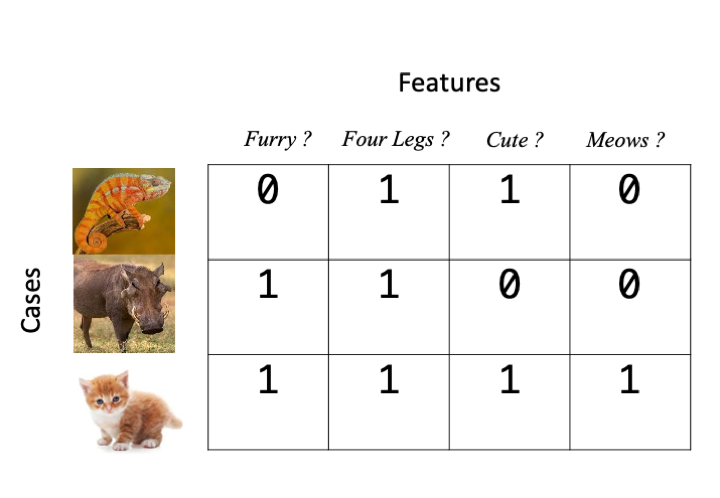
\includegraphics{figs/npmat.png}

Here's a gene expression based example, gene counts from an RNAseq experiment. The treatments are \(p\), the different genes are the \(n\)s

\begin{tabular}{l|r|r}
\hline
geneid & trt1 & trt2\\
\hline
gene1 & 9.313663 & 5.683347\\
\hline
gene2 & 16.824577 & 12.921582\\
\hline
gene3 & 11.134654 & 18.386286\\
\hline
gene4 & 18.245261 & 13.271525\\
\hline
gene5 & 19.107009 & 11.849221\\
\hline
\end{tabular}

Finally, here's a sequence based example

\begin{tabular}{l|l}
\hline
id & seq\\
\hline
gene1 & TESVI\\
\hline
gene2 & NESCI\\
\hline
gene3 & TESNI\\
\hline
gene4 & LEDVT\\
\hline
gene5 & ANDVI\\
\hline
\end{tabular}

In general ML tools need this to be true

\(n >> p\)

\(n\) must be much greater than \(p\). We must have many more cases than features we measured. Most ML tools will fail, or at least have reduced power when this isn't true. This can be a limiting factor in our ability to use ML. Conversely, the power will generally go up when it is true and very large data sets can give extraordinary ML power.

\hypertarget{clustering}{%
\section{Clustering}\label{clustering}}

The first class of ML tools we will look it is unsupervised clustering, this will be familiar to many biologists from heatmaps of gene expression data, but also more fundamentally from phylogenetic tree analysis. We'll look at a general overview before we look at some specific tools.

\hypertarget{the-distance-measure-and-matrix}{%
\subsection{The distance measure and matrix}\label{the-distance-measure-and-matrix}}

The first step of clustering is to get a measure of `distance' between all the pairs of cases \(n\)s that we have gathered. In this case when we say `distance', we mean a numeric measure of how similar or dissimilar our cases are. There are lots of different metrics of distance, e.g the correlation coefficient \(r\) is a measure of how similar two sets of numbers are. With this measure the higher the value, the more similar the cases are. Different types of data will need different distance metrics. For sequence based data we typically have the substitution or edit distance (the number of changes needed to make the two sequences identical).

The distance measure is a crucial step in clustering, but all tools have a sensible default and we don't need to worry about what it is \emph{exactly} at this stage beyond what we've discussed, but we do need to see what we do with the pairs of distances to understand the basics of the algorithm. Once we have the distances we form a distance matrix, which is always square, symmetrical across the diagonal and looks like this:

\begin{verbatim}
##       gene1 gene2 gene3 gene4 gene5
## gene1  0.00  1.00  0.87  1.00  0.96
## gene2  1.00  0.00  0.77  1.00  0.99
## gene3  0.87  0.77  0.00  0.97  1.00
## gene4  1.00  1.00  0.97  0.00  0.99
## gene5  0.96  0.99  1.00  0.99  0.00
\end{verbatim}

As we can see, the further apart the genes expression across the treatments the greater the distance measure. Once we have this matrix the clustering can begin.

\hypertarget{hierarchical-single-linkage-clustering}{%
\section{Hierarchical (single linkage) Clustering}\label{hierarchical-single-linkage-clustering}}

Hierarchical clustering is the most common and straightforward clustering algorithm. The elements (cases or \(n\)s) are formed into the distance matrix and the aim is to group the pair of elements with the smallest distance into one, then repeat, continuing until we run out of elements. We then move onto grouping the pairs and so on until there's nothing left to group. Allison Horst demonstrates it better than I, so here's the excellent illustrations she made that run through the process.

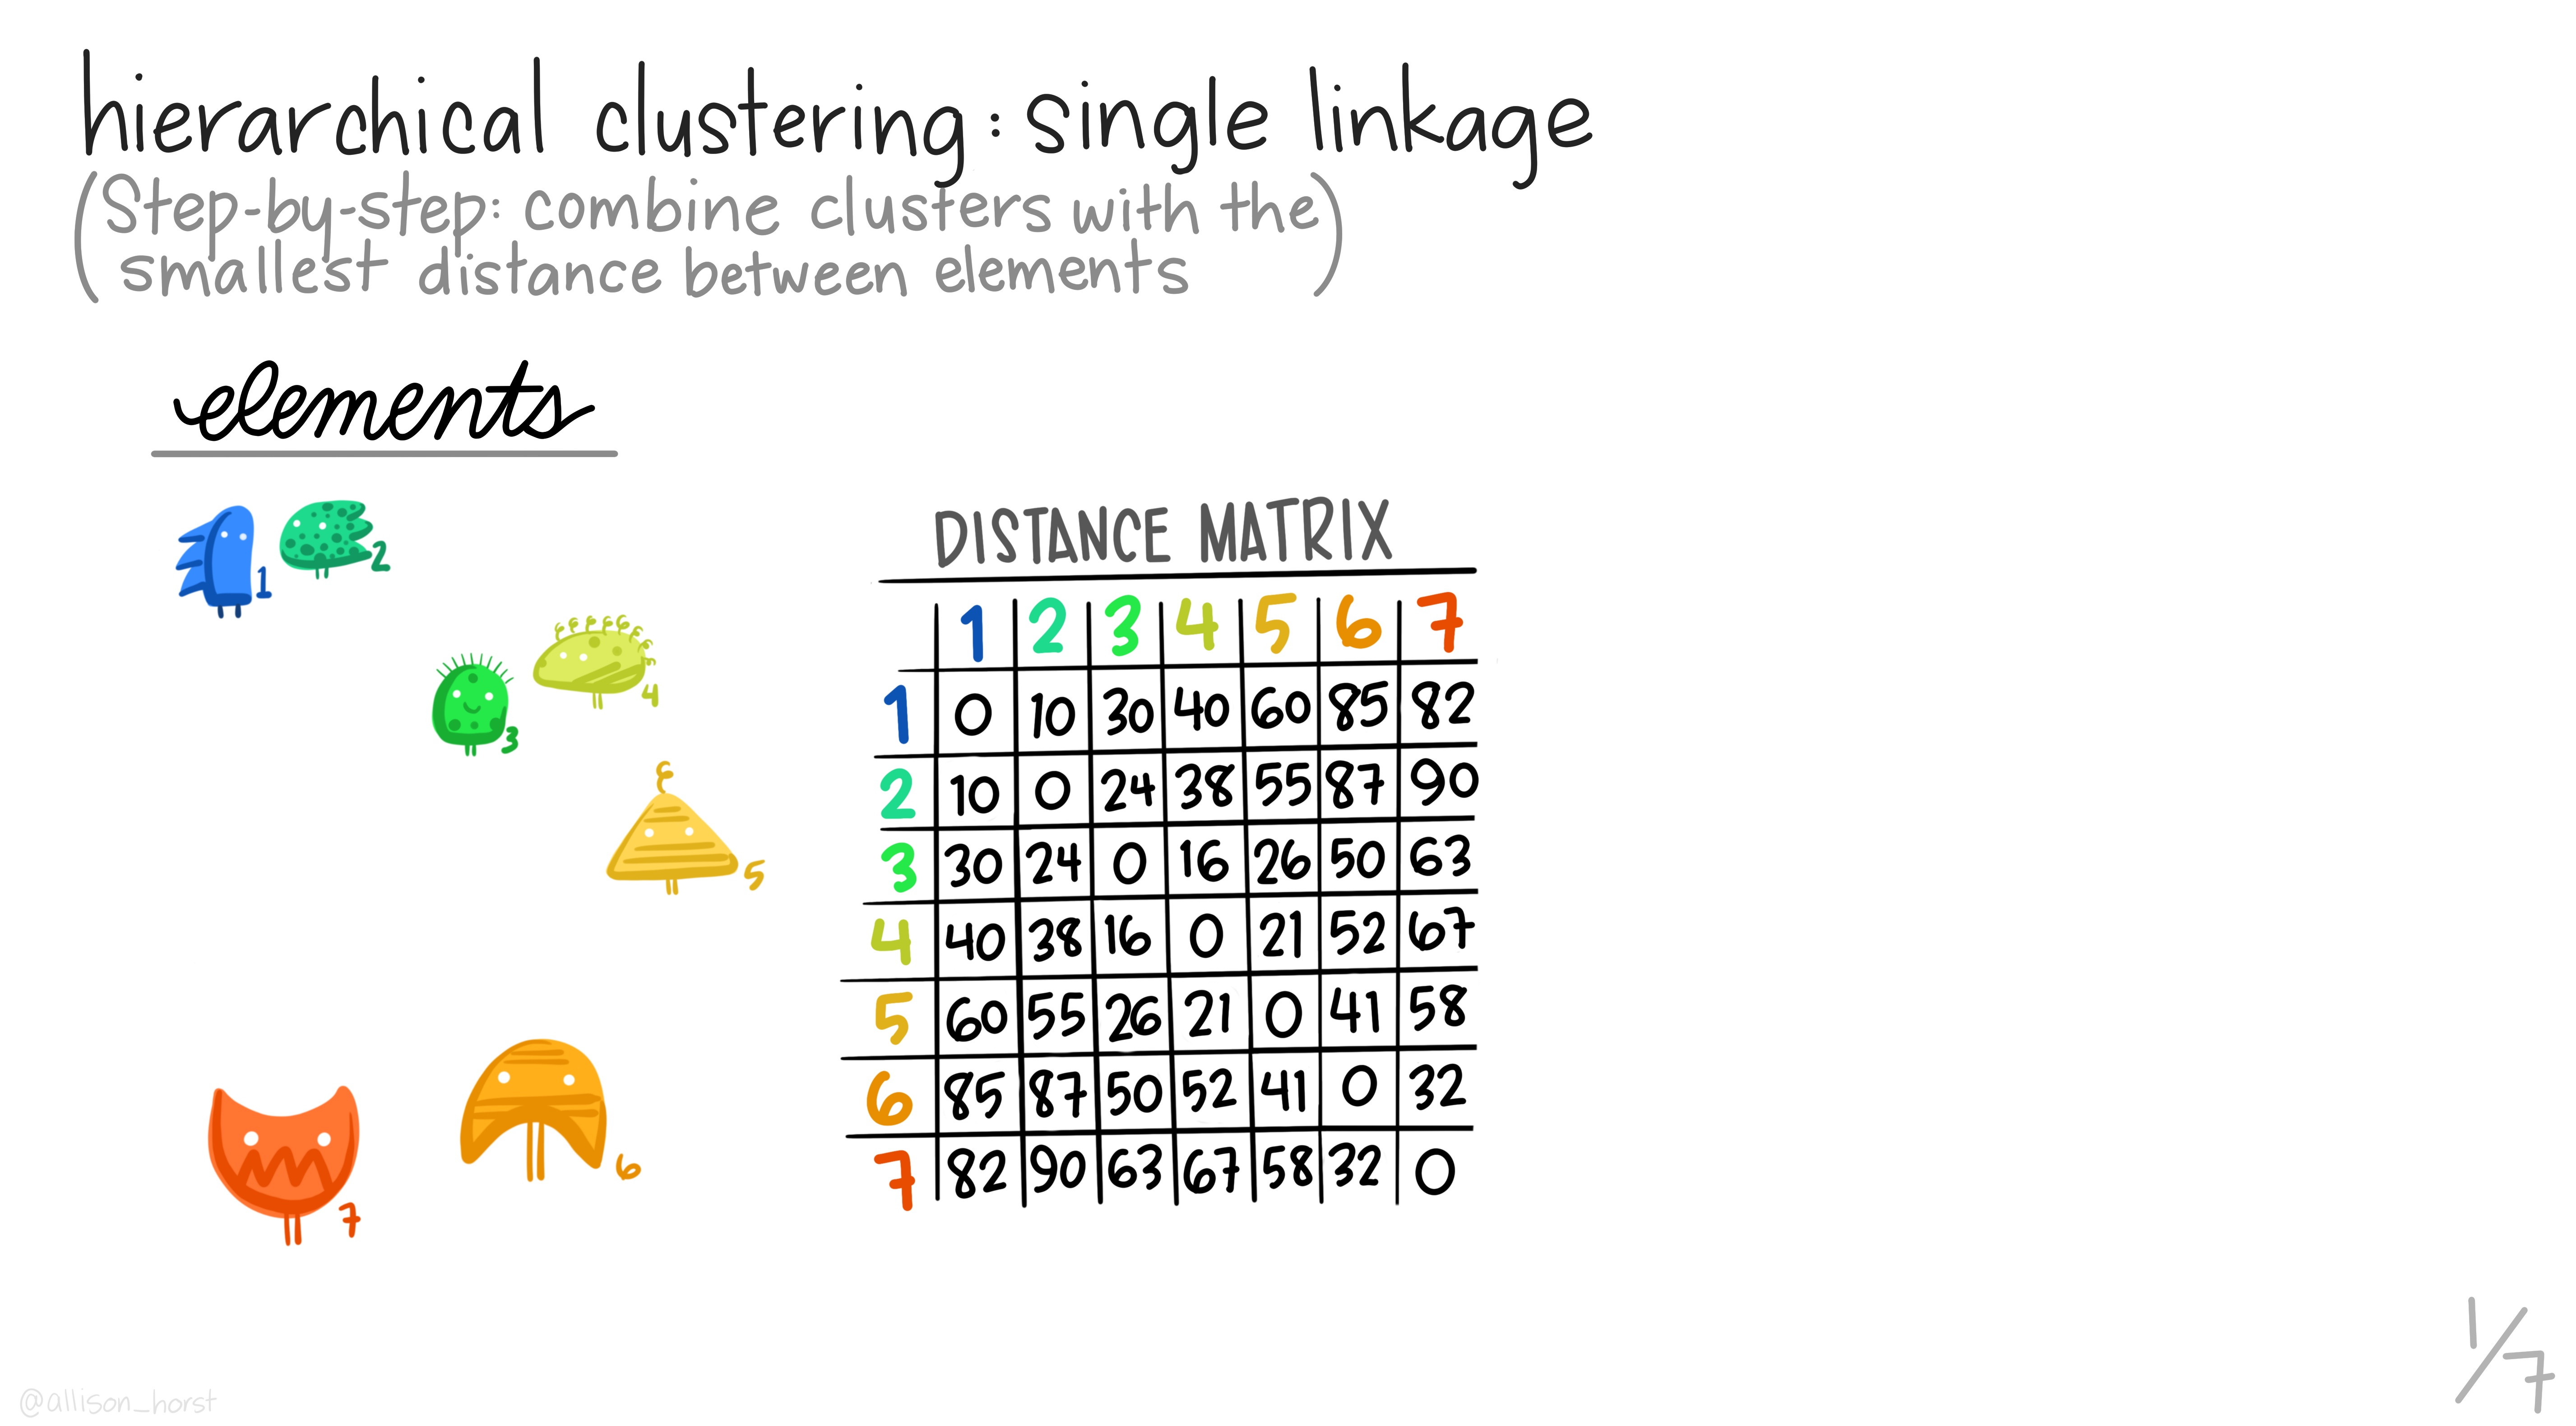
\includegraphics{figs/cluster_single_linkage_1.jpg} 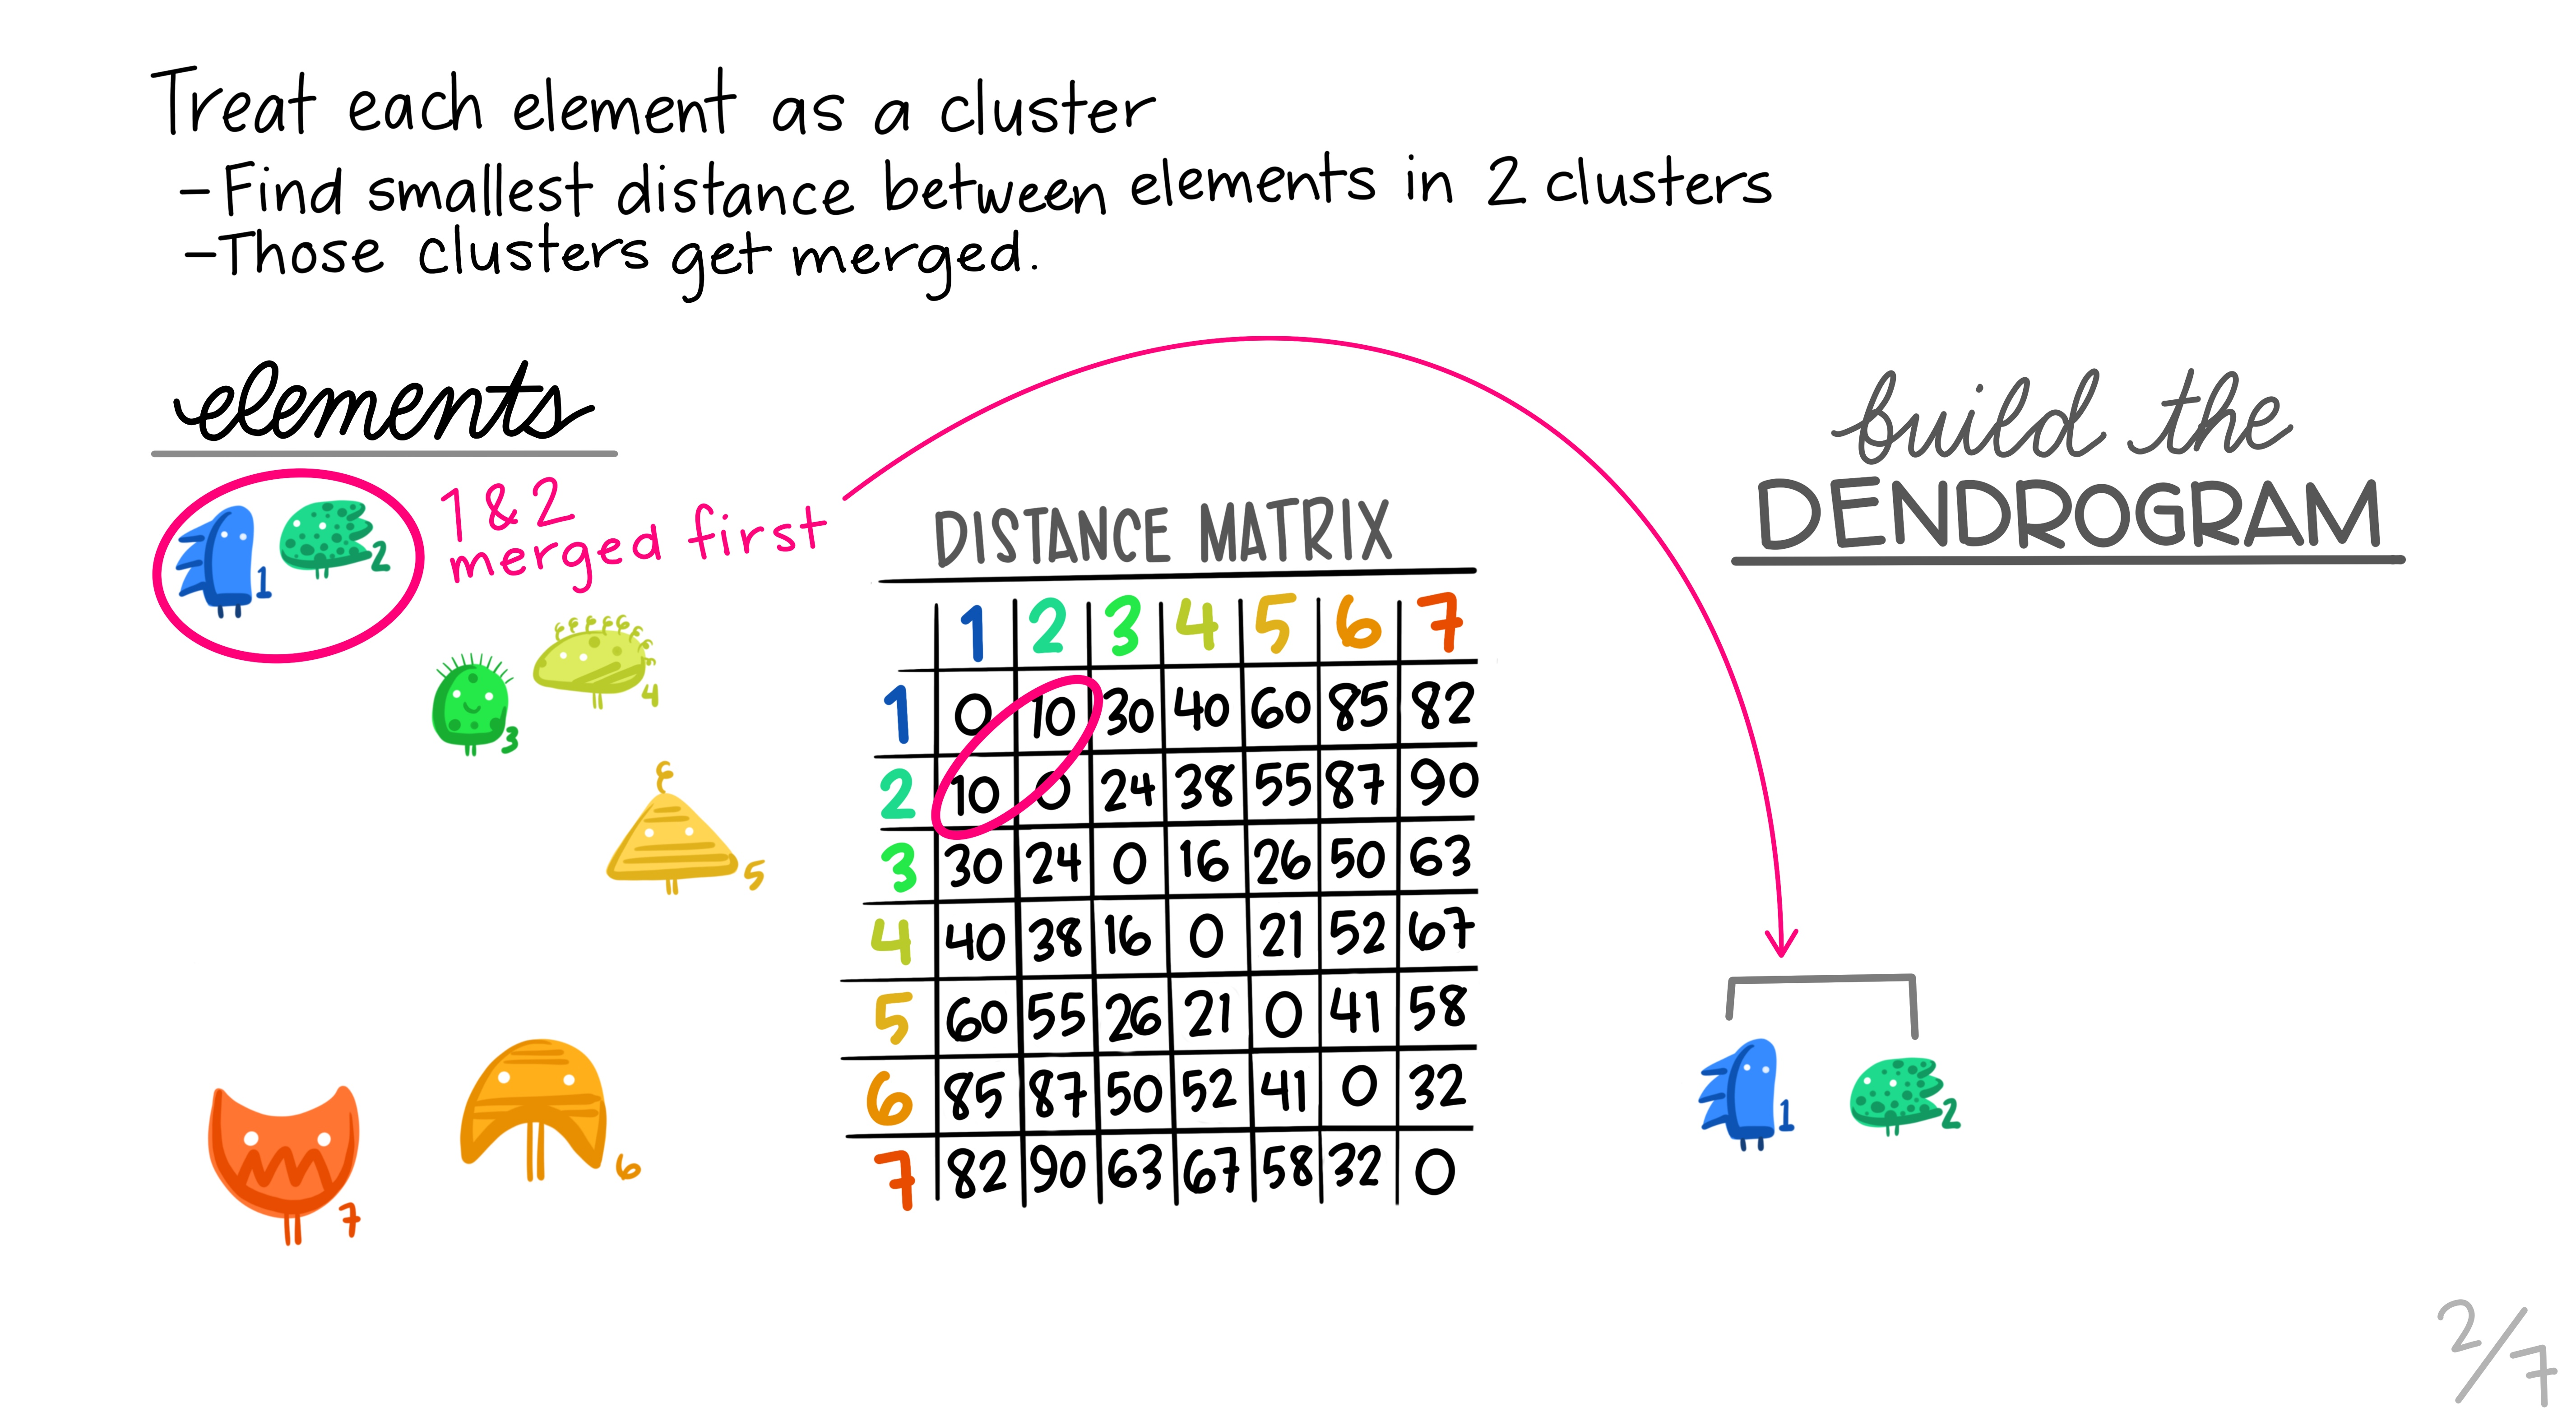
\includegraphics{figs/cluster_single_linkage_2.jpg} 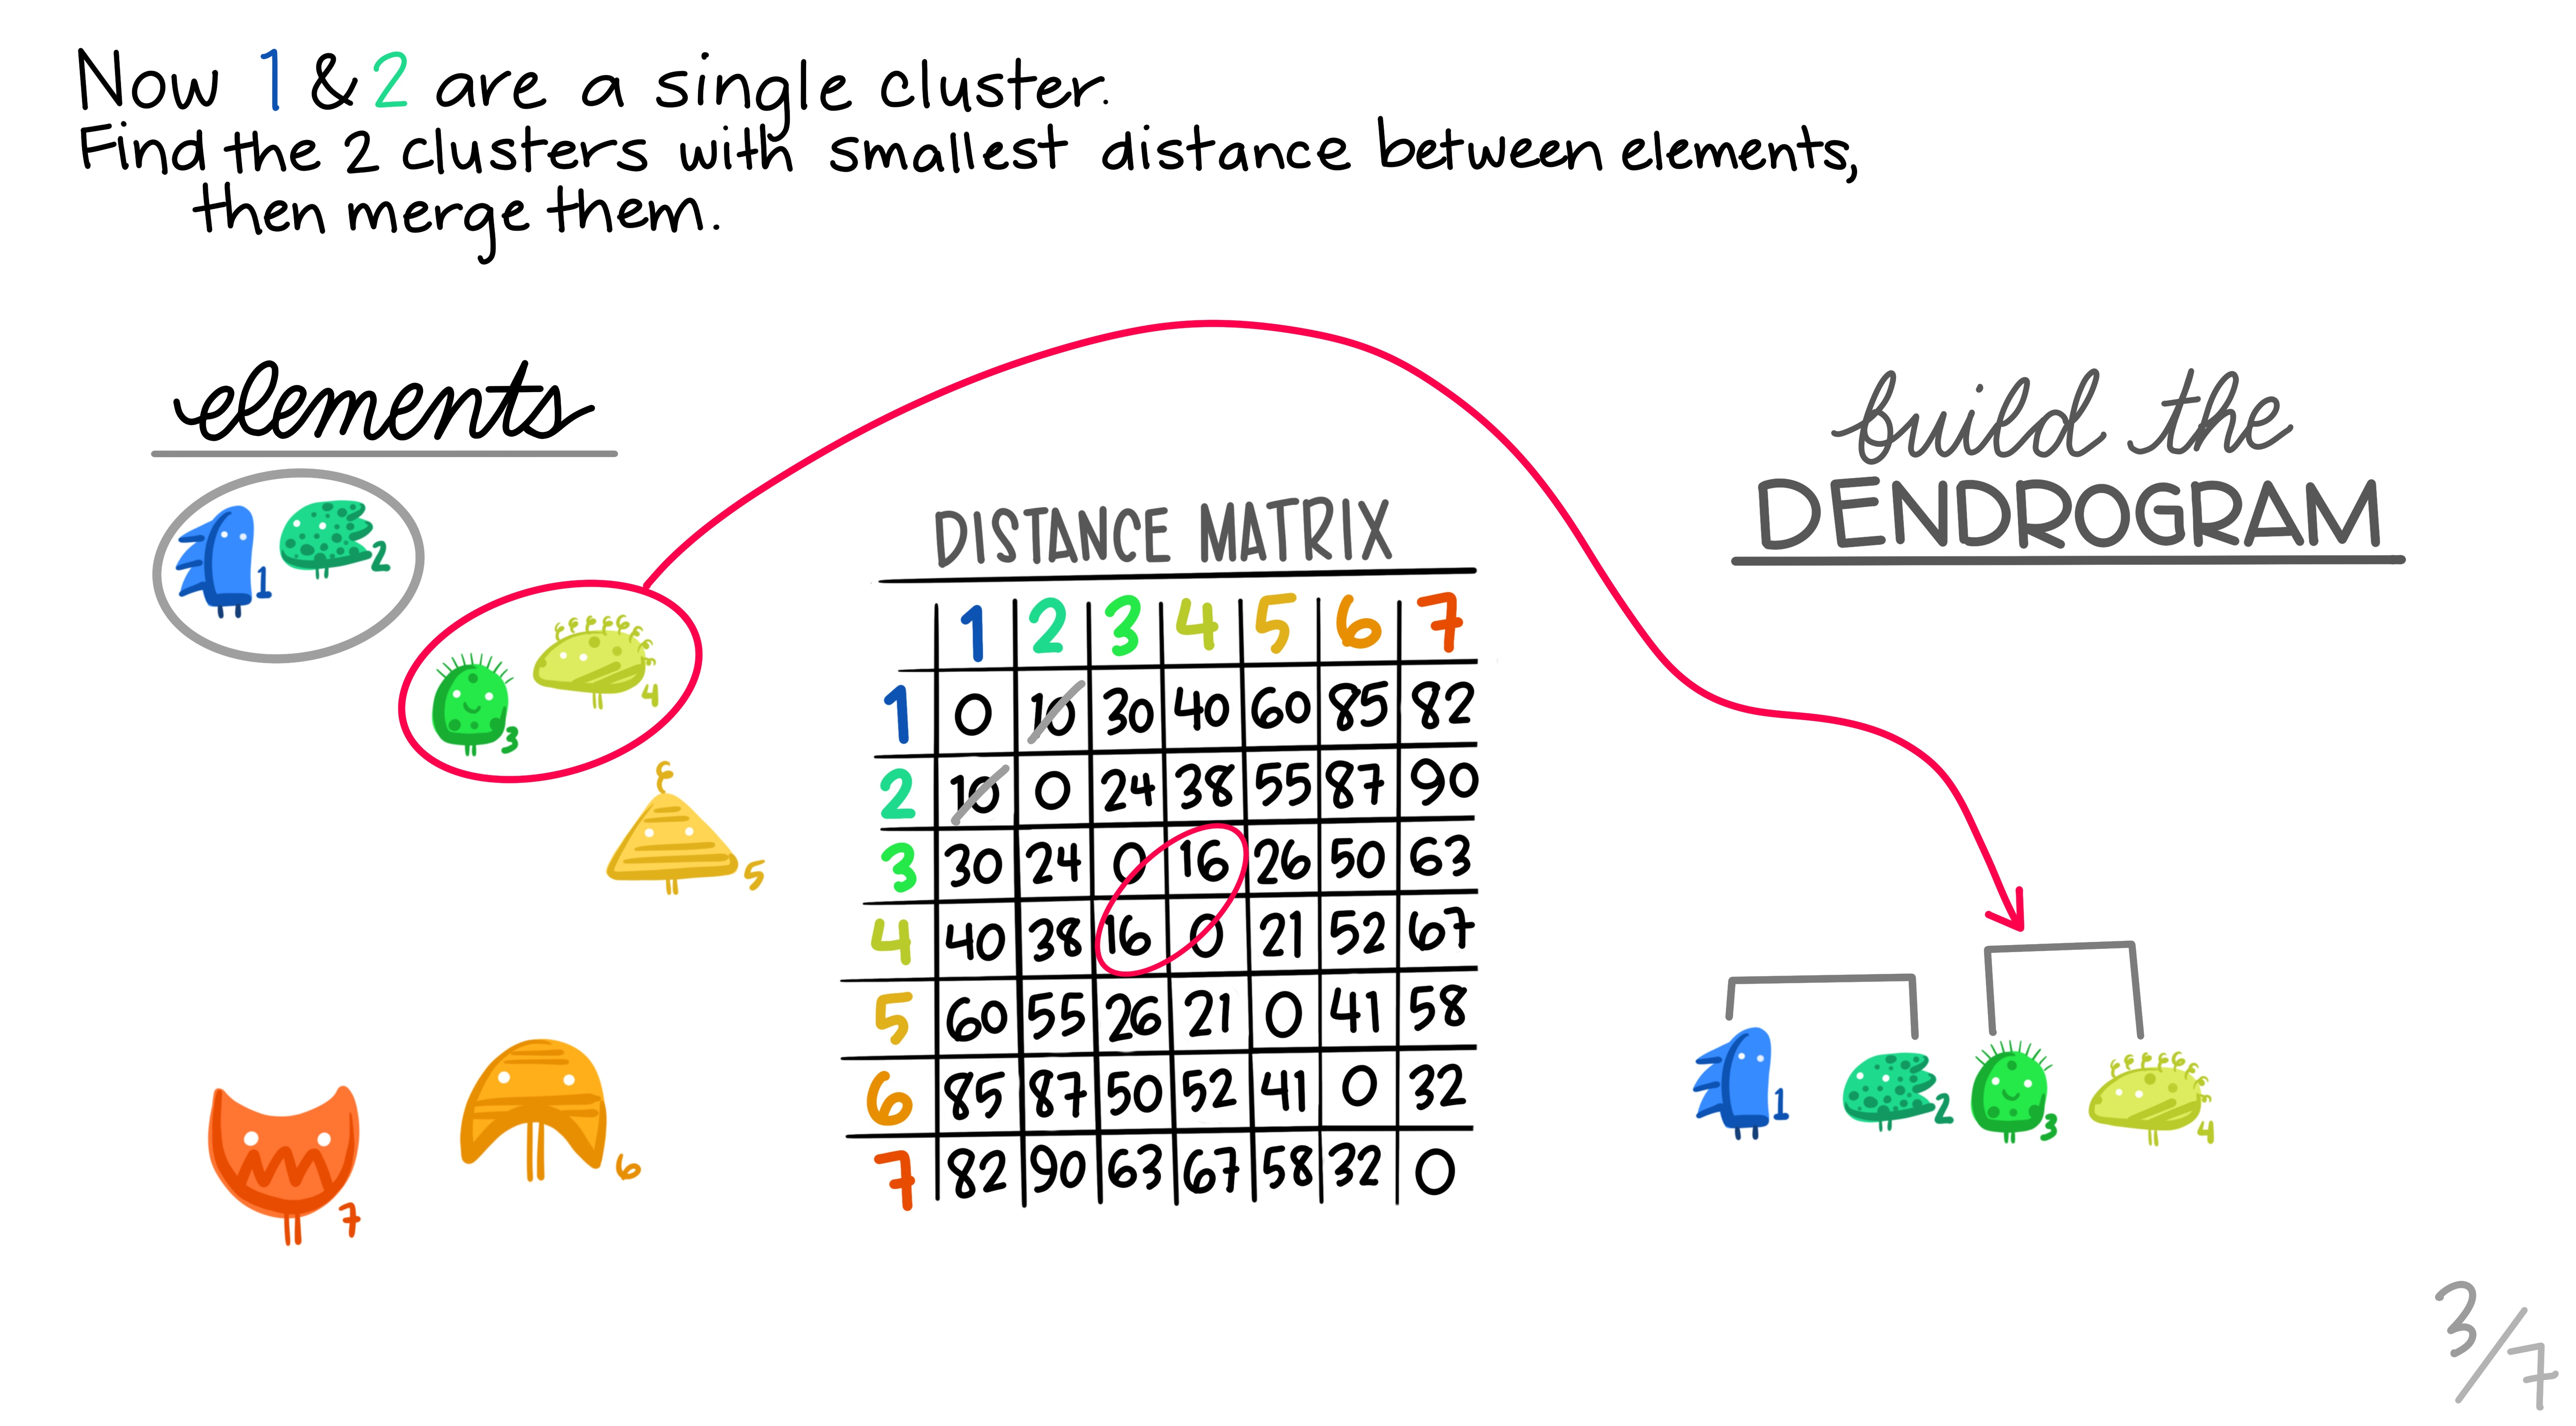
\includegraphics{figs/cluster_single_linkage_3.jpg} 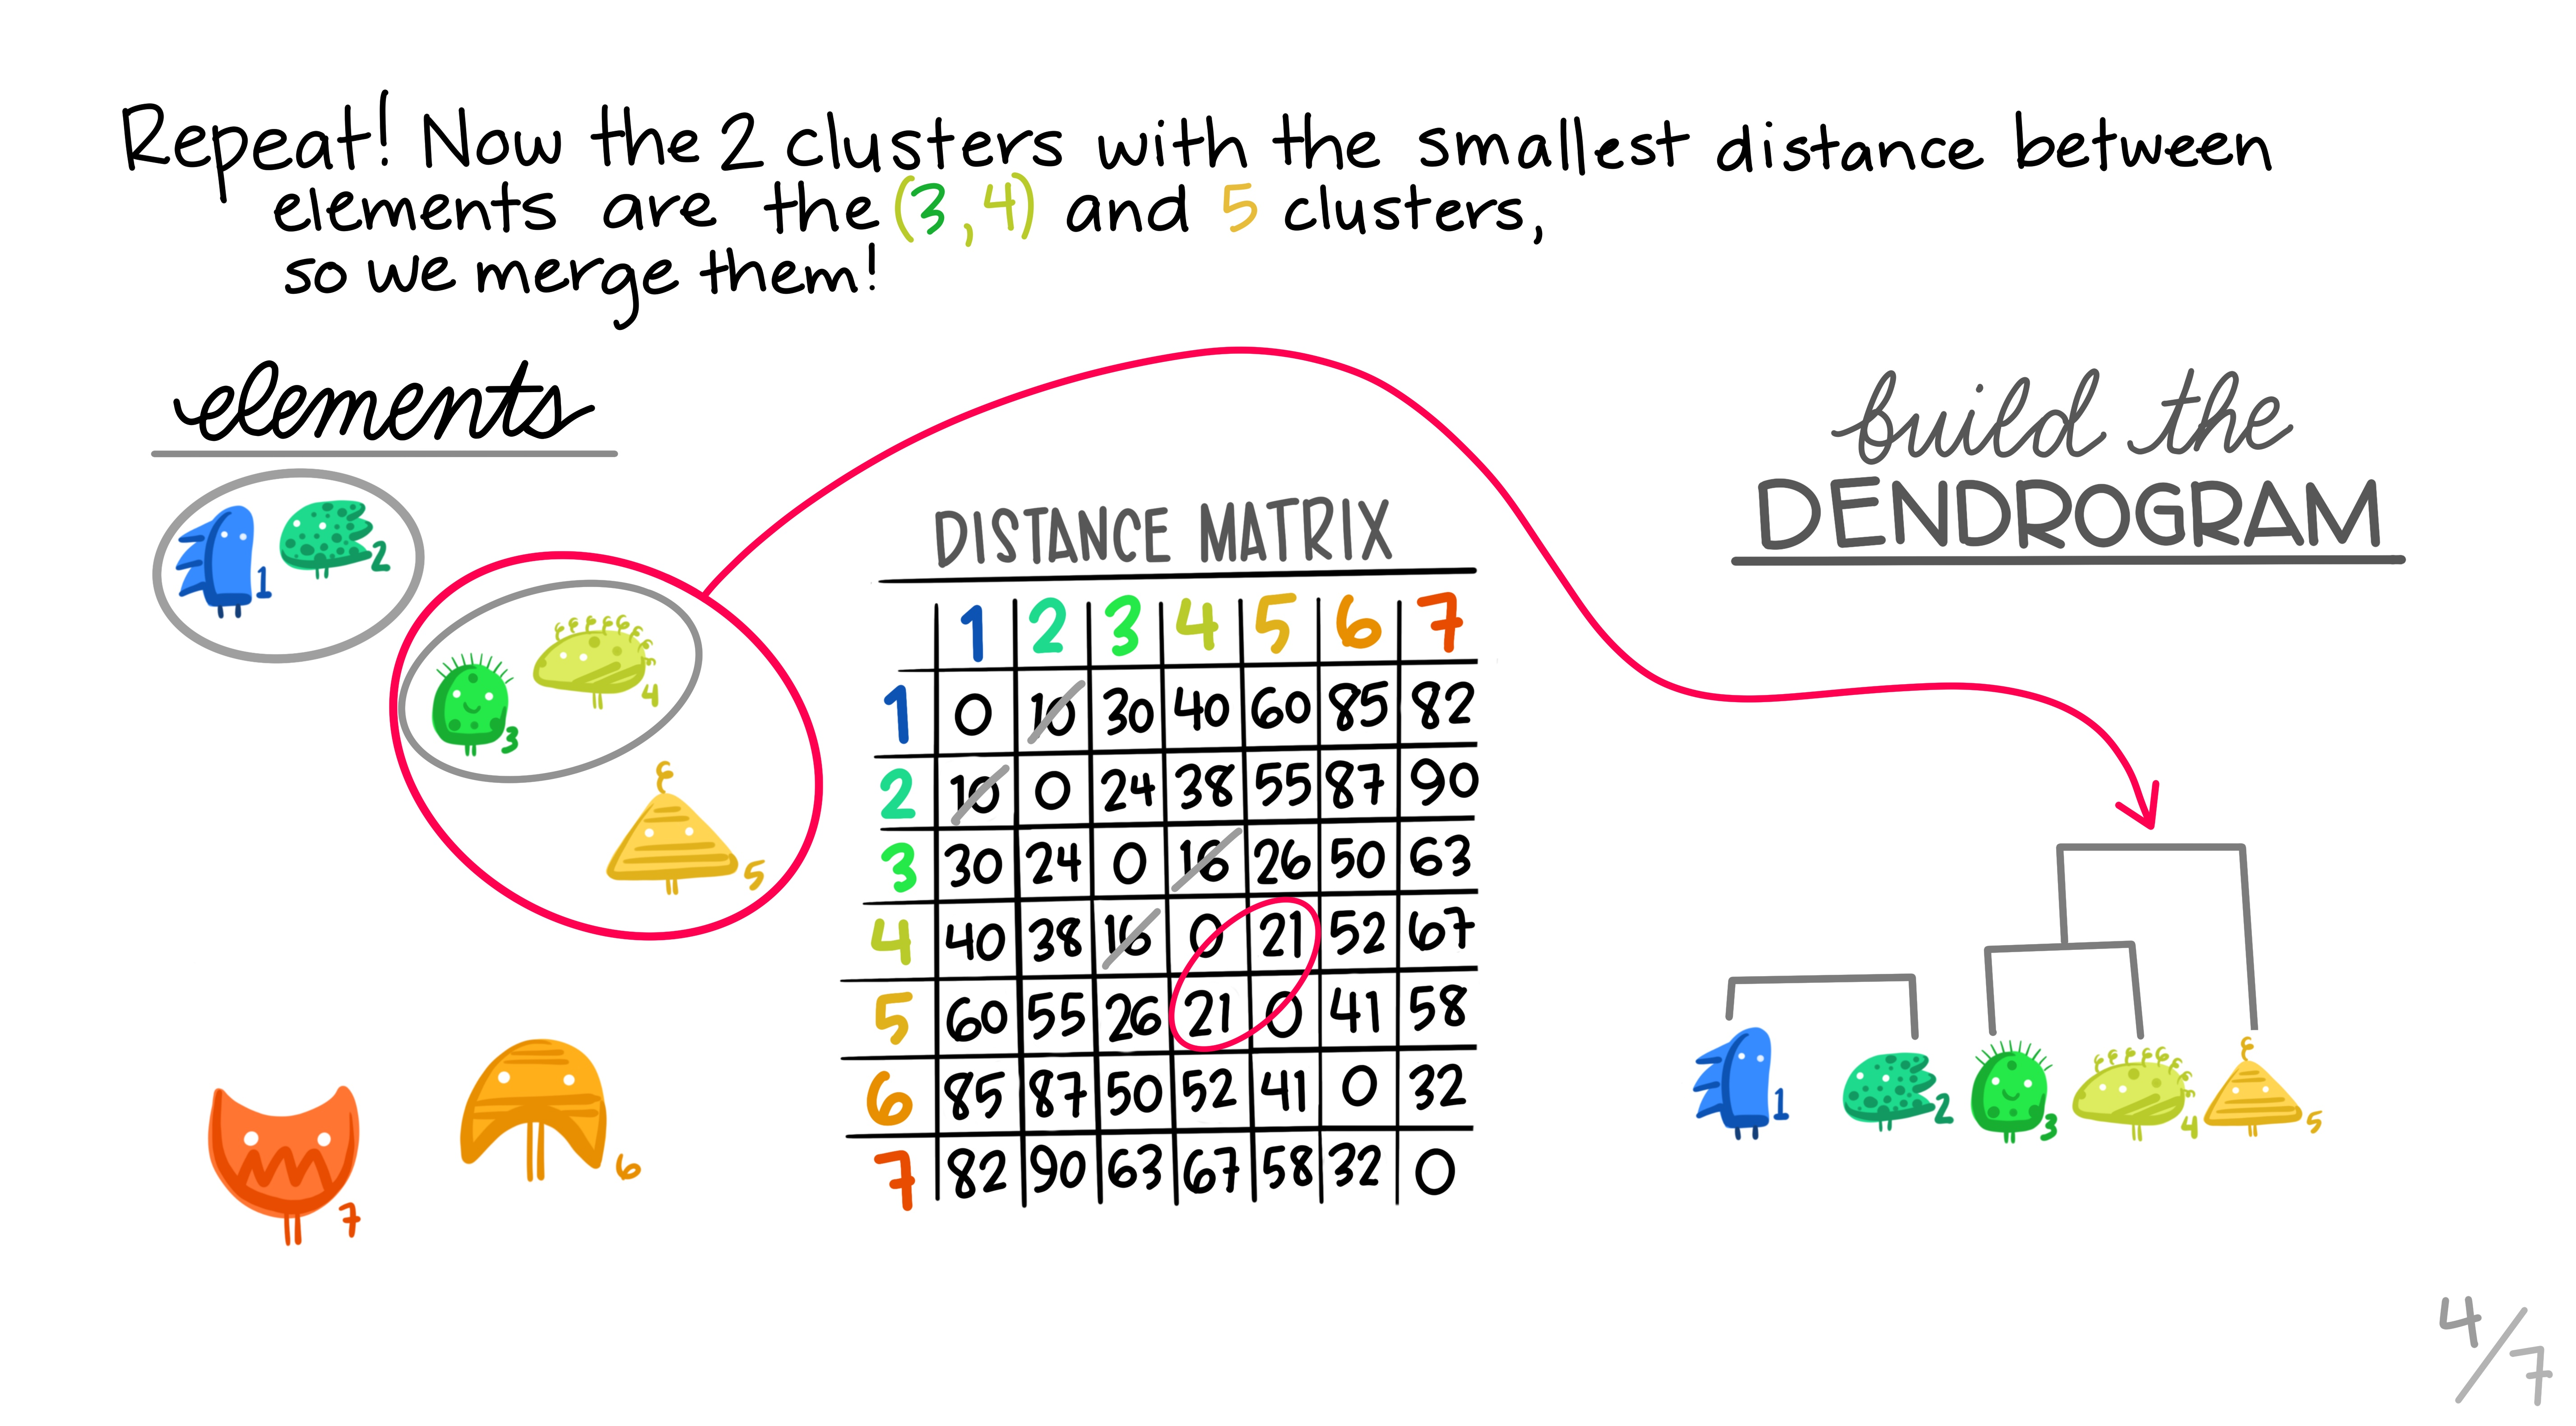
\includegraphics{figs/cluster_single_linkage_4.jpg} 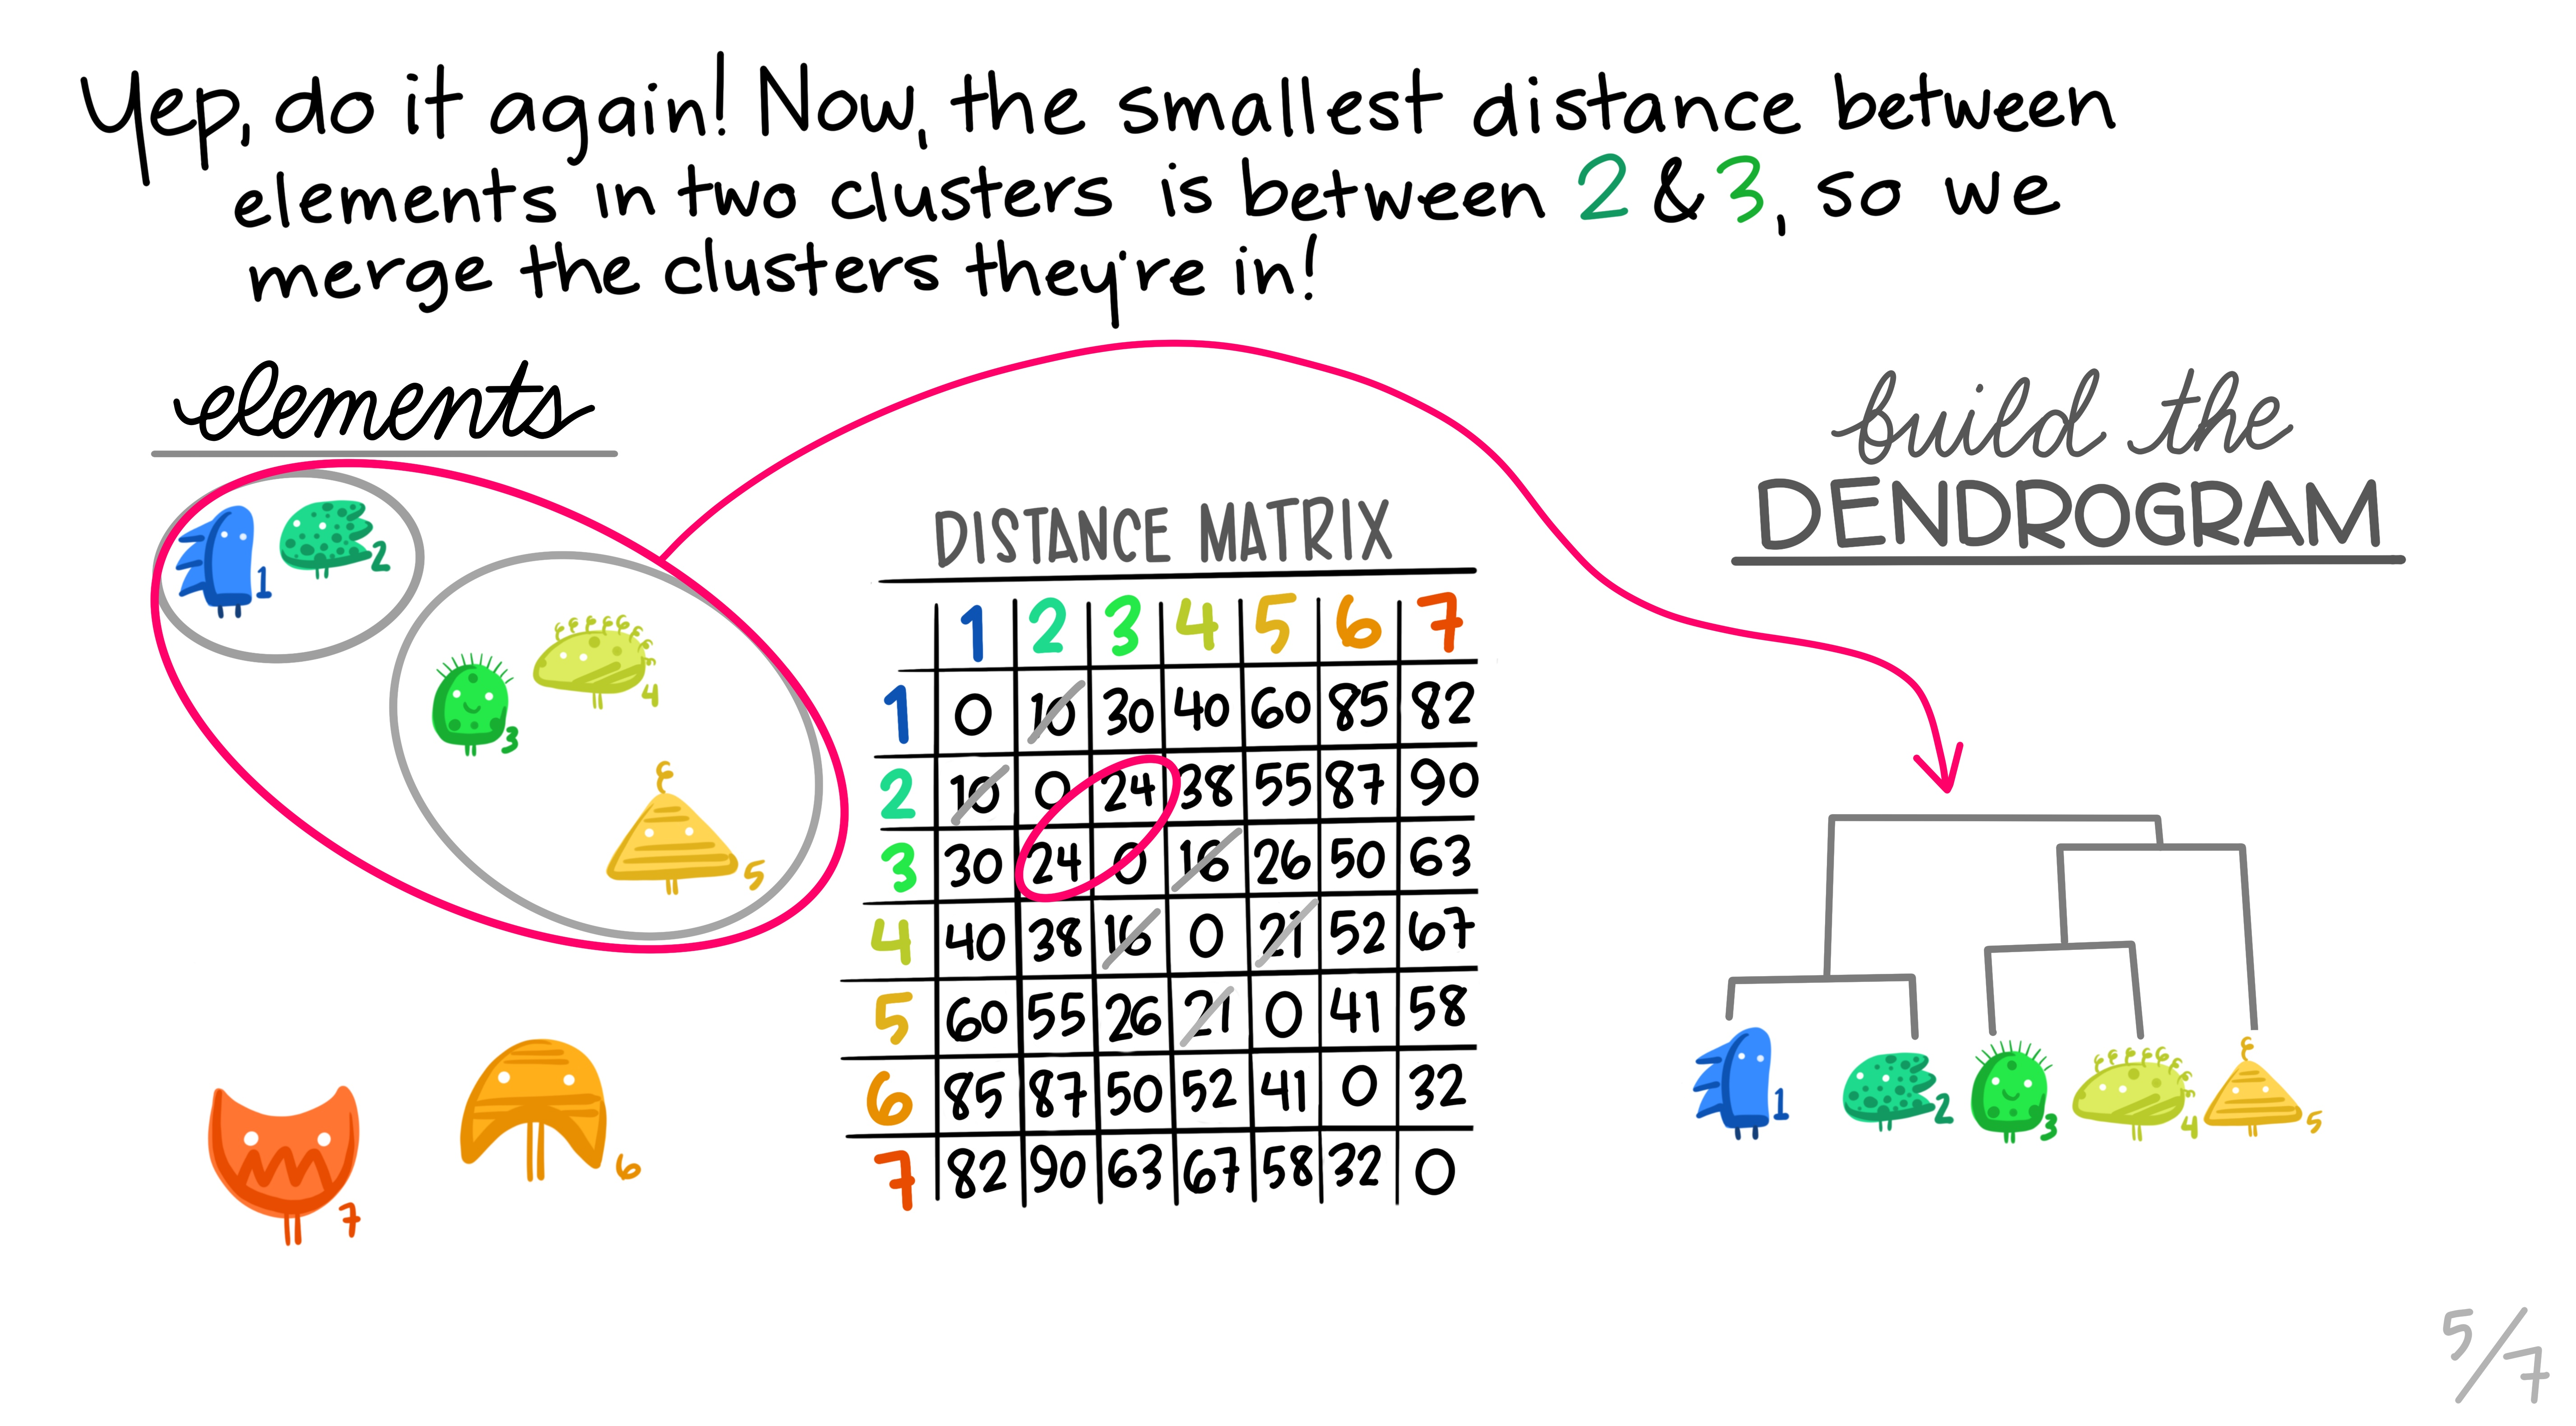
\includegraphics{figs/cluster_single_linkage_5.jpg} 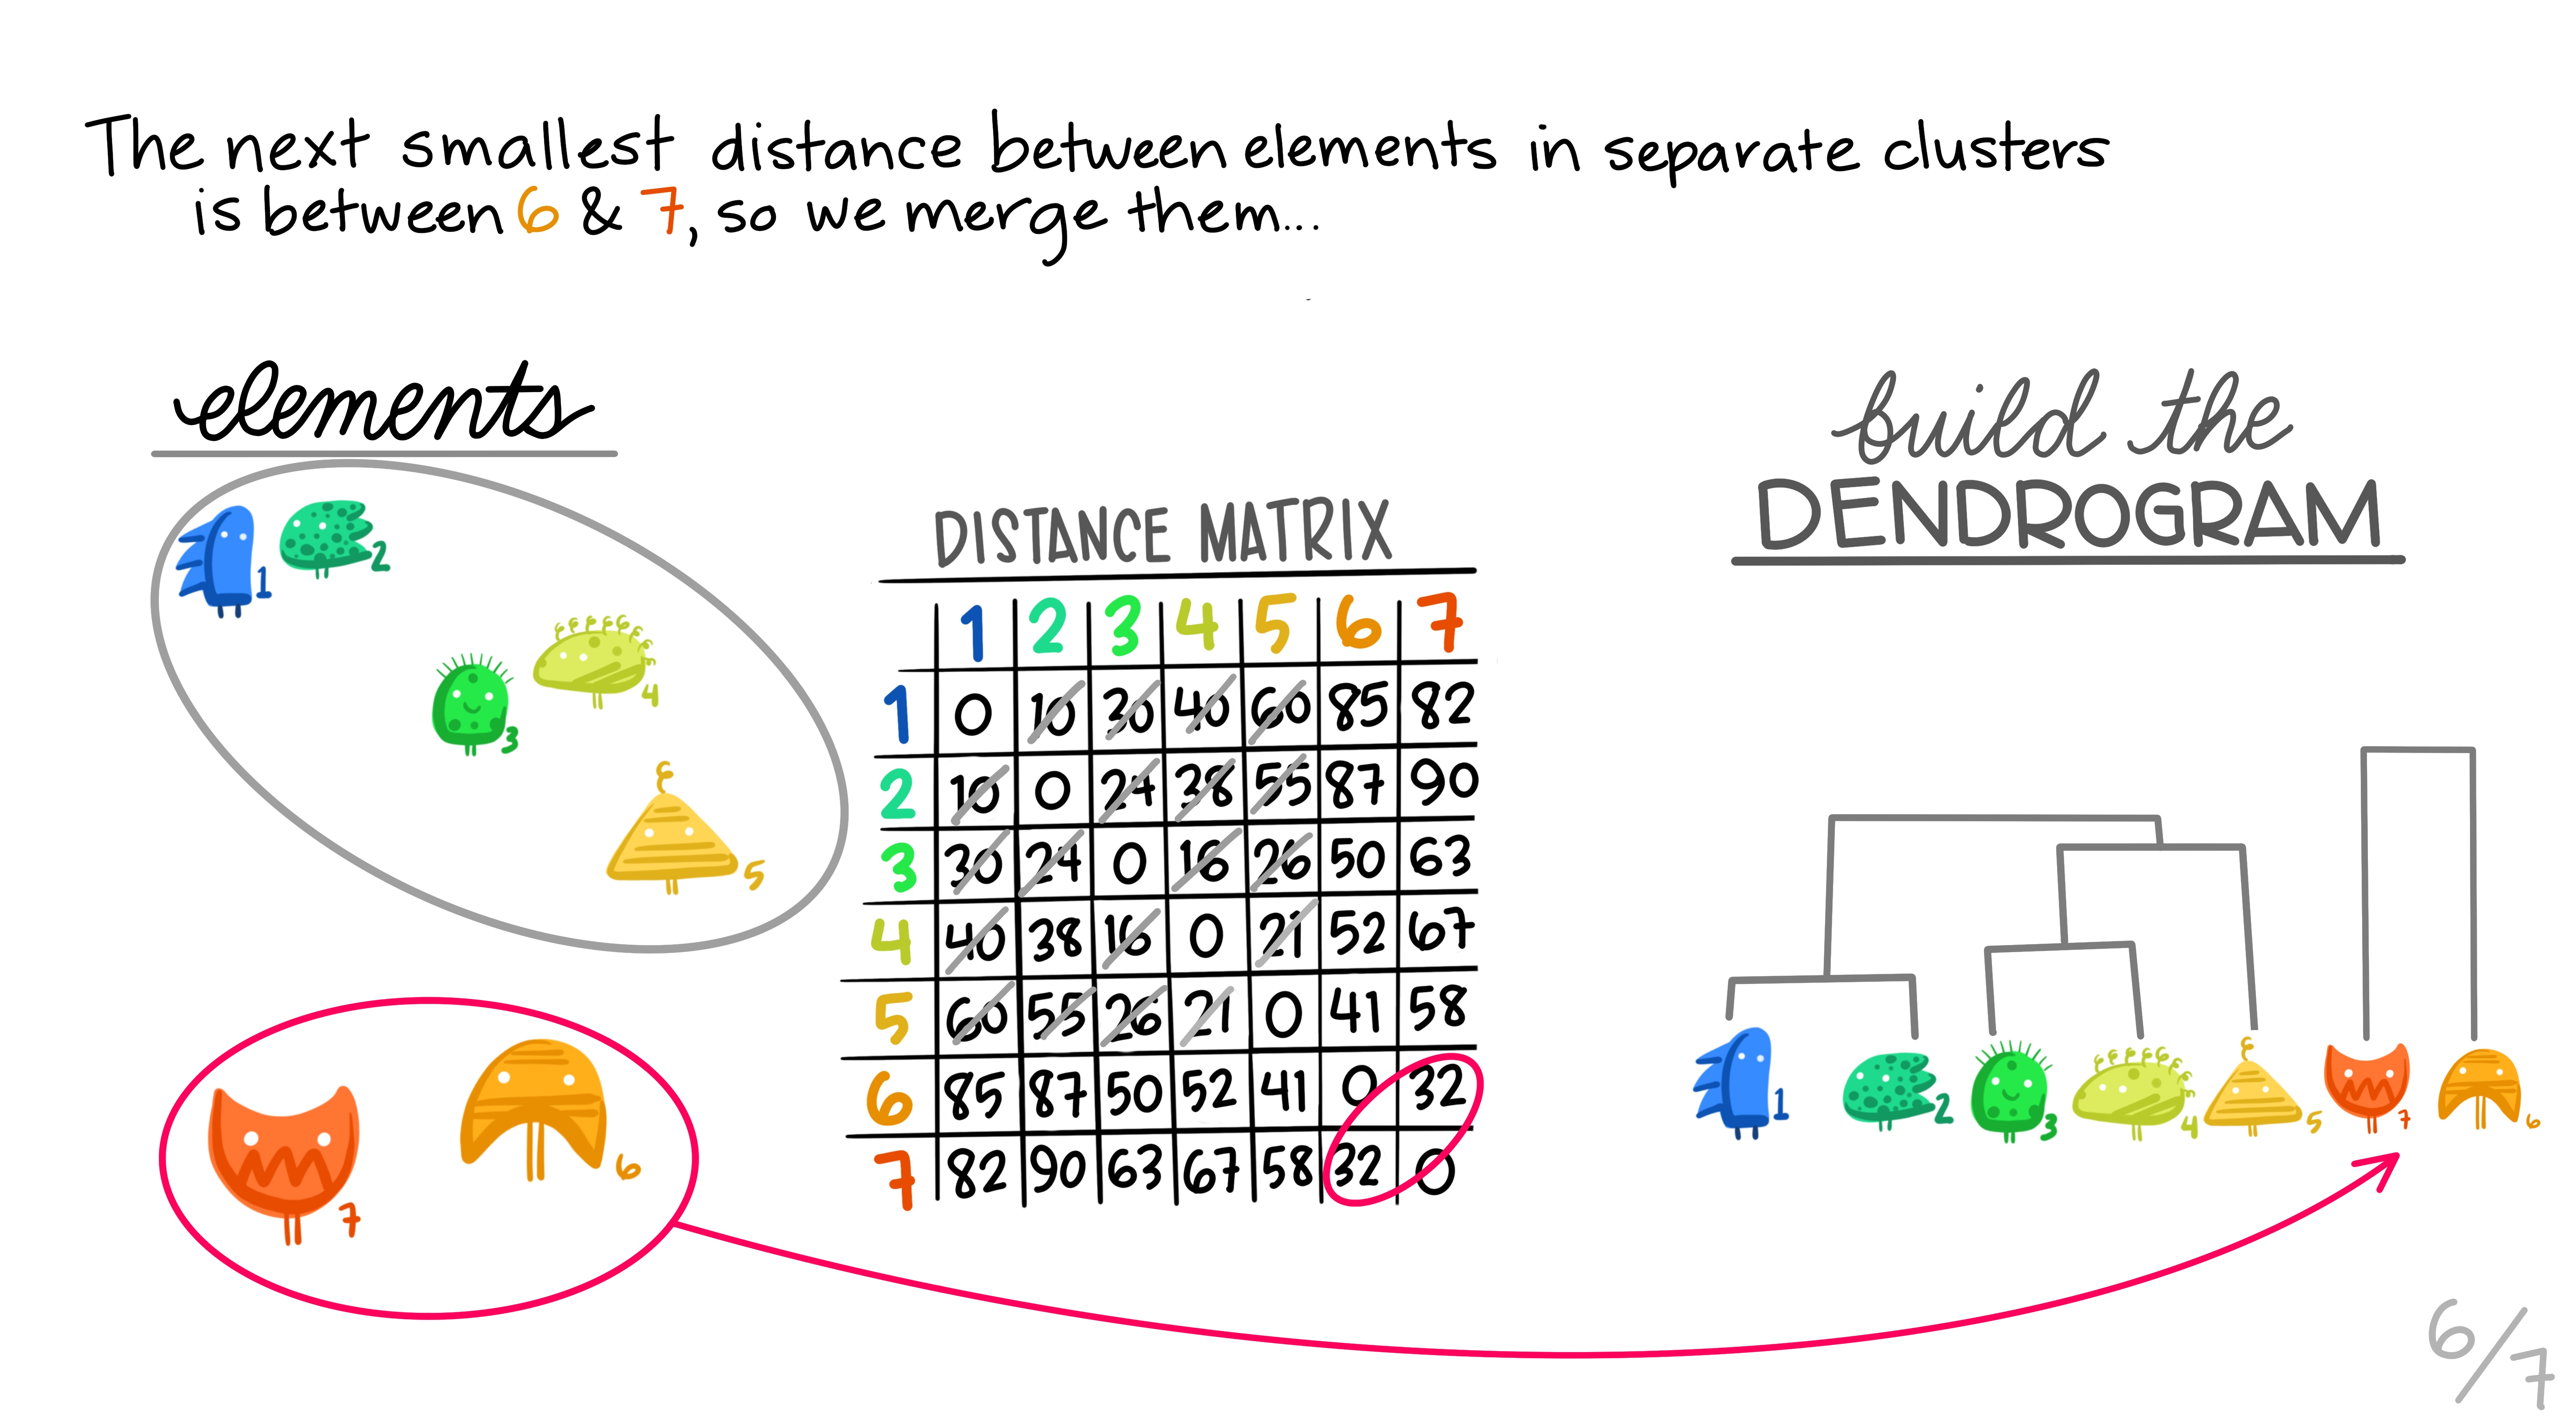
\includegraphics{figs/cluster_single_linkage_6.jpg} 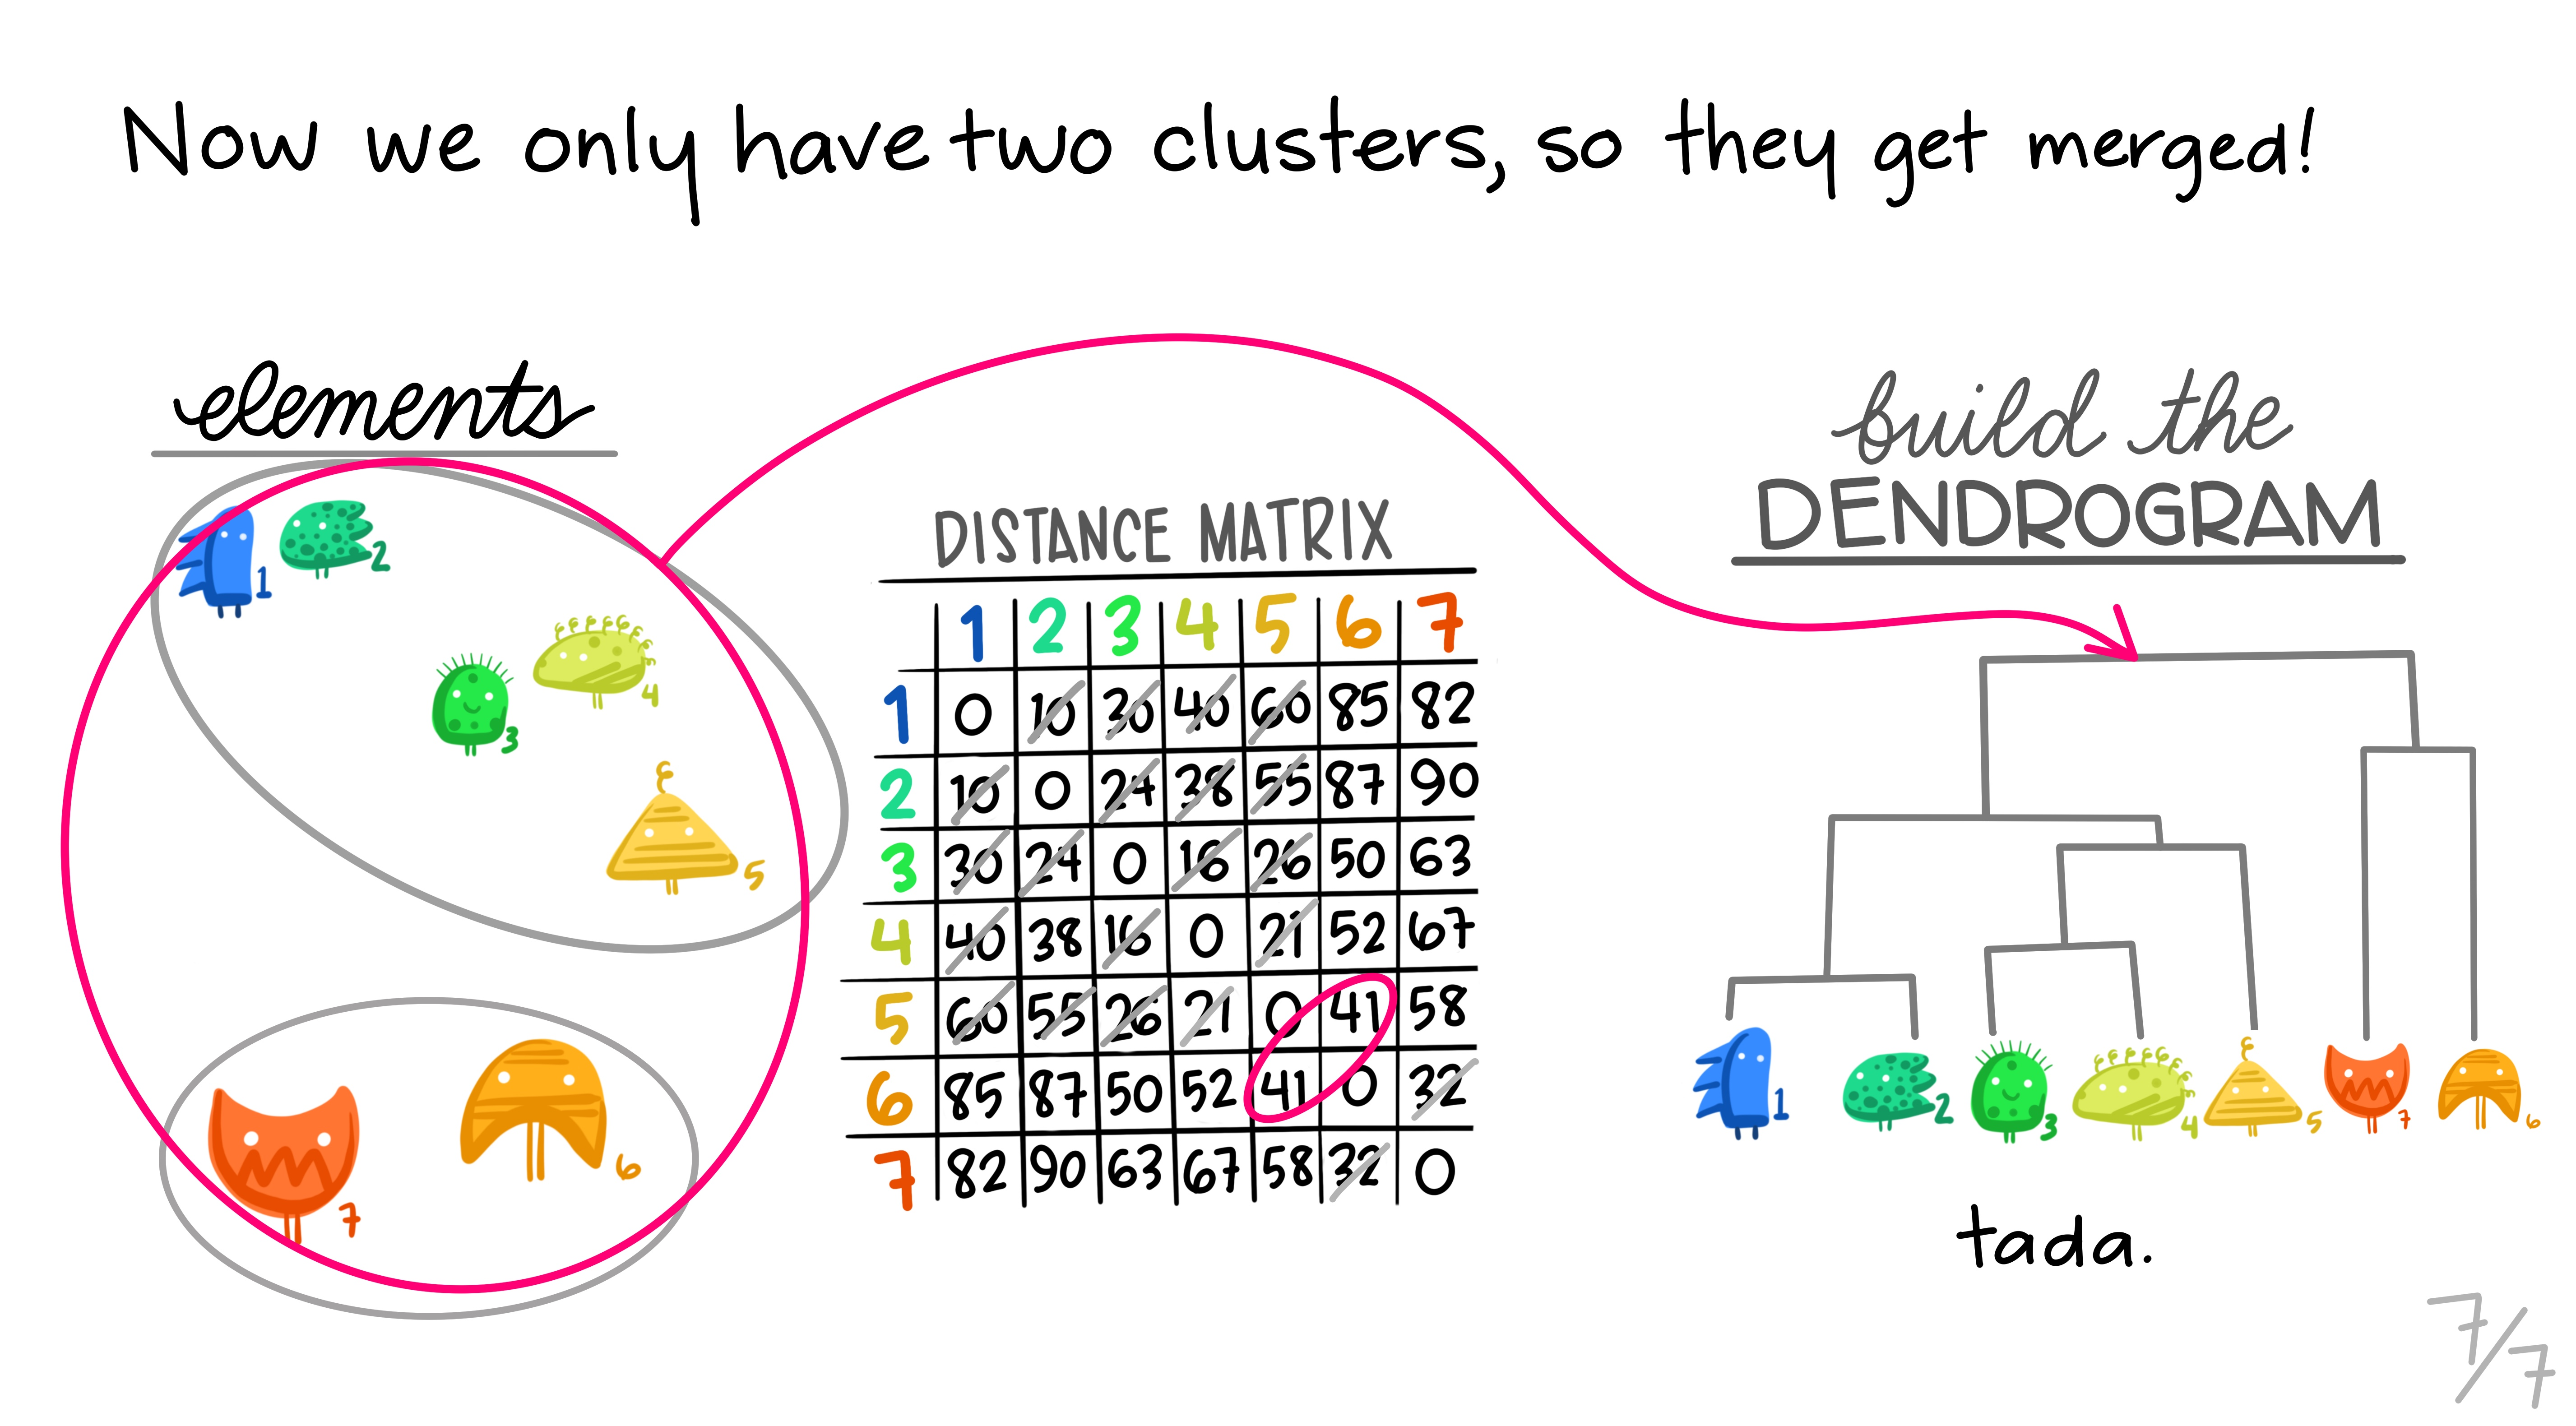
\includegraphics{figs/cluster_single_linkage_7.jpg}

Hopefully this montage has clarified the overall process of grouping elements based on distance metrics calculated between all pairs. The question remains though, how can we do this in R?

\hypertarget{hierarchical-clustering-in-base-r}{%
\subsection{Hierarchical clustering in Base R}\label{hierarchical-clustering-in-base-r}}

There is an \texttt{hclust()} function built into R we can use. Being part of the base distribution and not using any packages means that this function is a bit general and needs data in particular format. Specifically it needs a numbers only matrix or data frame of information - you'd need to remove all text information from the object - getting this in to shape is left as an exercise for the reader. You would end up with a matrix object looking something like this

\begin{Shaded}
\begin{Highlighting}[]
\NormalTok{data_mat}
\end{Highlighting}
\end{Shaded}

\begin{verbatim}
##            trt1      trt2
## gene1  9.313663  5.683347
## gene2 16.824577 12.921582
## gene3 11.134654 18.386286
## gene4 18.245261 13.271525
## gene5 19.107009 11.849221
\end{verbatim}

You can the get clusters by creating the \texttt{dist} object with the \texttt{dist} function and the clusters with \texttt{hclust()} using the method \texttt{single} to apply the single linkage clustering we learned above. Then we can directly plot the dendrogram.

\begin{Shaded}
\begin{Highlighting}[]
\NormalTok{data_dist <-}\StringTok{ }\KeywordTok{dist}\NormalTok{(data_mat, }\DataTypeTok{diag=}\OtherTok{TRUE}\NormalTok{)}
\NormalTok{clusters <-}\StringTok{ }\KeywordTok{hclust}\NormalTok{(data_dist, }\DataTypeTok{method=}\StringTok{"single"}\NormalTok{)}
\KeywordTok{plot}\NormalTok{(clusters)}
\end{Highlighting}
\end{Shaded}

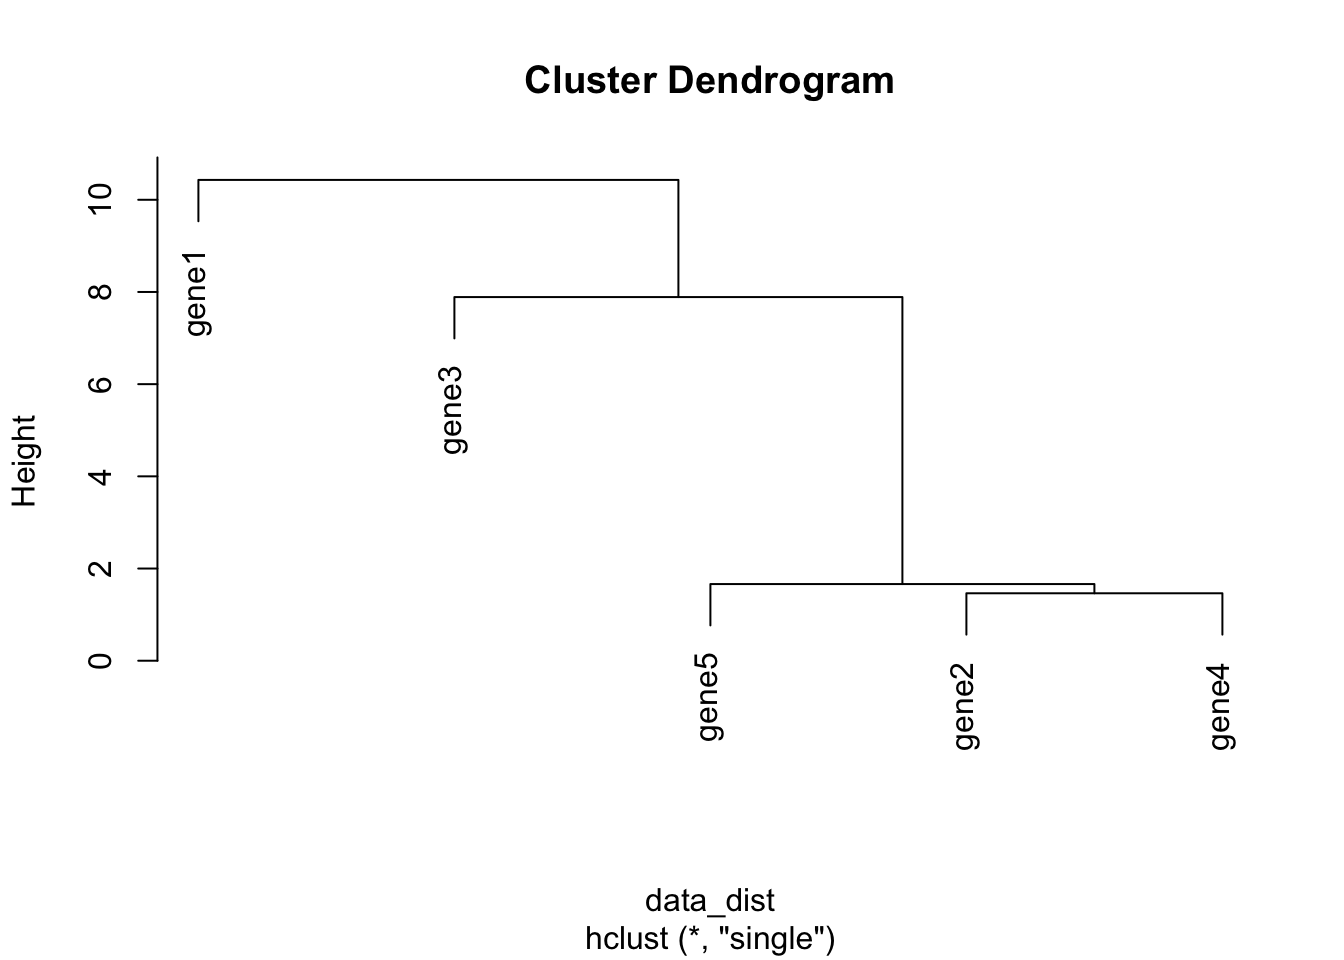
\includegraphics{machine_learning_files/figure-latex/unnamed-chunk-26-1.pdf}

Note that the distance measure by default is \texttt{euclidean} which is a different way of computing distances than the \(r\) correlation coefficient we discussed earlier. \texttt{euclidean} is more commonly used, but it's beyond the scope of this course to discuss distance measures in detail. More information on distance measures is freely available on \href{https://en.wikipedia.org/wiki/Distance}{Wikipedia}.

\hypertarget{clustered-heatmaps}{%
\subsection{Clustered Heatmaps}\label{clustered-heatmaps}}

Typically you'll want to make some sort of heatmap and have a tree or dendrogram of the clusters stuck on the side, rather than just have a cluster tree on its own. Again, base R has a helpful if general function, \texttt{heatmap()}, simply pass the matrix object e.g \texttt{data\_mat} and it can do the rest.

\begin{Shaded}
\begin{Highlighting}[]
\KeywordTok{heatmap}\NormalTok{(data_mat)}
\end{Highlighting}
\end{Shaded}

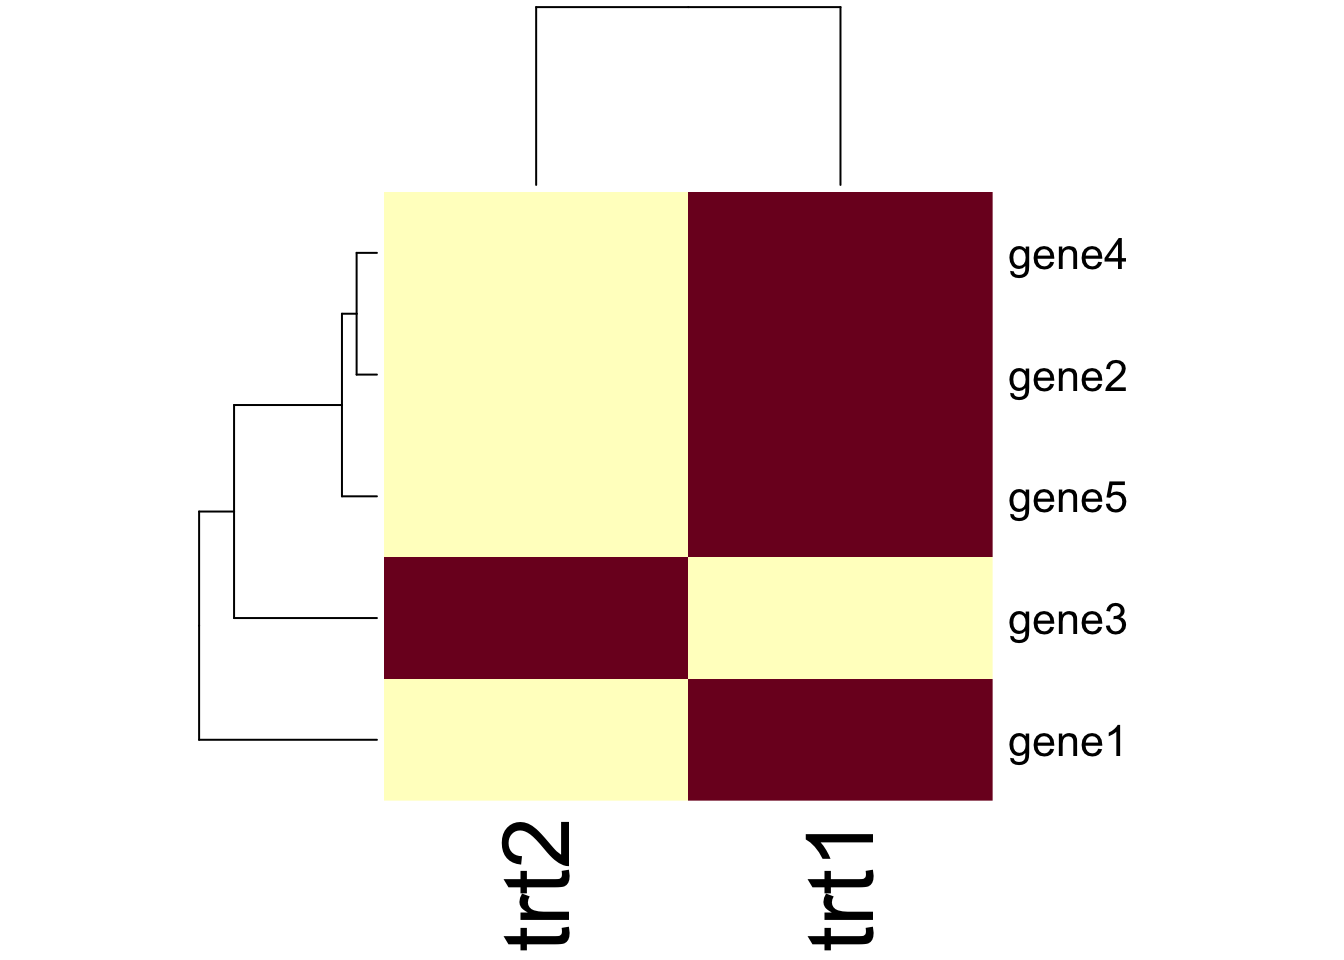
\includegraphics{machine_learning_files/figure-latex/unnamed-chunk-27-1.pdf}

The function has a lot of customisation options, which you can investigate using \texttt{?heatmap} and Google!

\hypertarget{extra-credit-ggplot-and-clusters}{%
\subsection{Extra Credit: ggplot and clusters}\label{extra-credit-ggplot-and-clusters}}

Heatmaps can be drawn in \texttt{ggplot} using the \texttt{geom\_tile()} geom. If our data are in `tidy' format like this

\begin{Shaded}
\begin{Highlighting}[]
\NormalTok{tidy_gdf}
\end{Highlighting}
\end{Shaded}

\begin{verbatim}
## # A tibble: 10 x 3
##    geneid treatment expression
##    <chr>  <chr>          <dbl>
##  1 gene1  trt1            9.31
##  2 gene1  trt2            5.68
##  3 gene2  trt1           16.8 
##  4 gene2  trt2           12.9 
##  5 gene3  trt1           11.1 
##  6 gene3  trt2           18.4 
##  7 gene4  trt1           18.2 
##  8 gene4  trt2           13.3 
##  9 gene5  trt1           19.1 
## 10 gene5  trt2           11.8
\end{verbatim}

We can make a heatmap quite simply, like this

\begin{Shaded}
\begin{Highlighting}[]
\KeywordTok{library}\NormalTok{(ggplot2)}
\NormalTok{hmap <-}\StringTok{ }\KeywordTok{ggplot}\NormalTok{(tidy_gdf) }\OperatorTok{+}\StringTok{ }\KeywordTok{aes}\NormalTok{(treatment, geneid) }\OperatorTok{+}\StringTok{ }\KeywordTok{geom_tile}\NormalTok{(}\KeywordTok{aes}\NormalTok{(}\DataTypeTok{fill=}\NormalTok{expression))}
\NormalTok{hmap}
\end{Highlighting}
\end{Shaded}

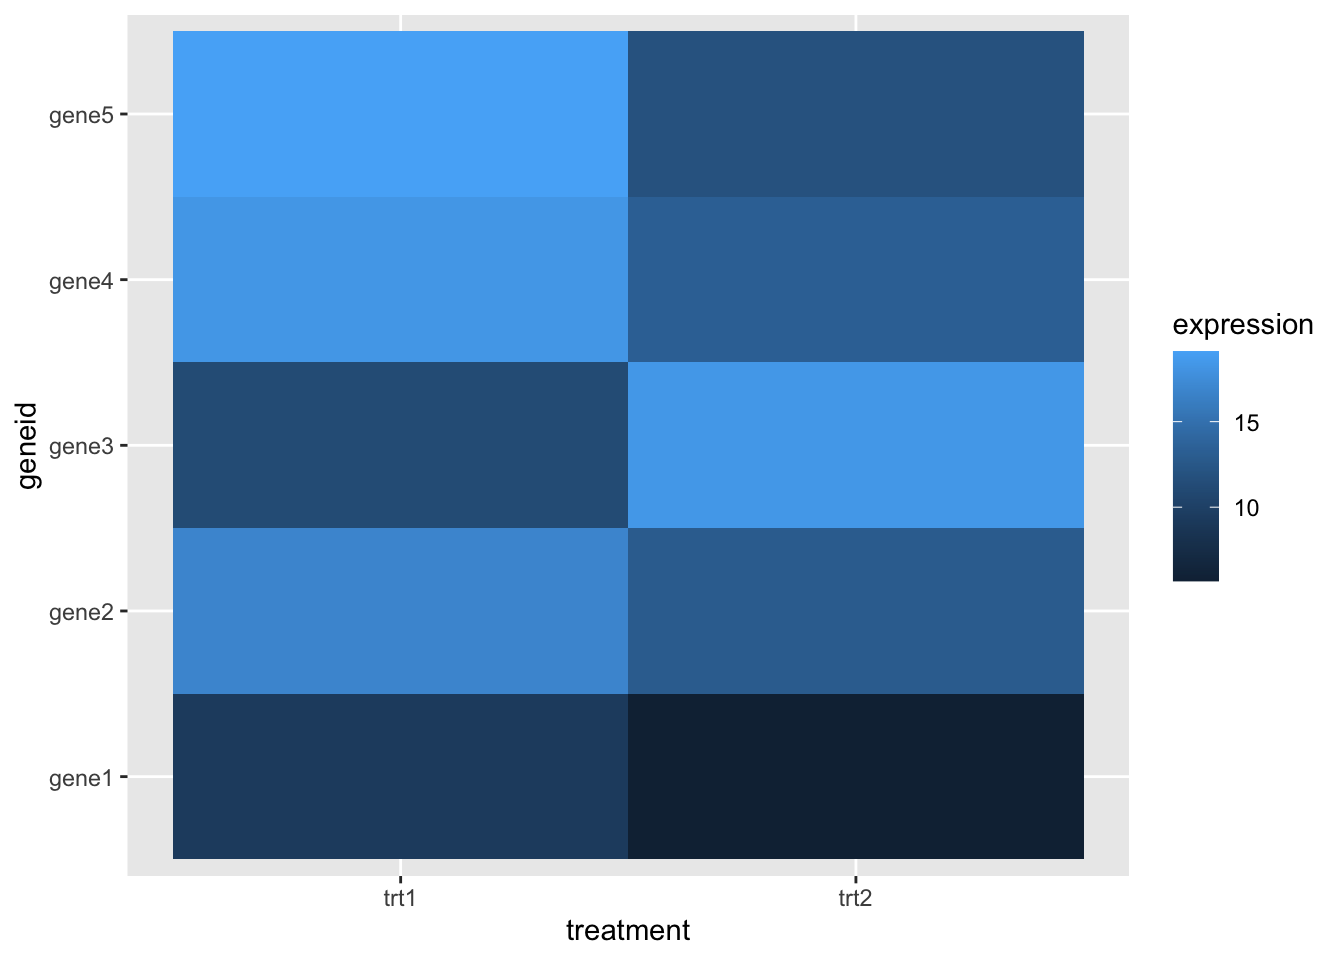
\includegraphics{machine_learning_files/figure-latex/unnamed-chunk-30-1.pdf}

But this has no dendrogram and is not clustered! It's going to take a little fiddling to add this on - we can get the clusters out of the \texttt{hclust()} result and apply those. To do that we must solve another problem first - turning our tidy data into a matrix! That can be done with \texttt{pivot\_wider()} from \texttt{tidyr}, which gets us most of the way there.

\begin{Shaded}
\begin{Highlighting}[]
\KeywordTok{library}\NormalTok{(tidyr)}
\NormalTok{wide_gdf <-}\StringTok{ }\NormalTok{tidy_gdf }\OperatorTok\StringTok{ }\KeywordTok{pivot_wider}\NormalTok{(}
  \DataTypeTok{id_cols =} \StringTok{"geneid"}\NormalTok{, }
  \DataTypeTok{names_from=}\StringTok{"treatment"}\NormalTok{, }
  \DataTypeTok{values_from=}\StringTok{"expression"}\NormalTok{)}
\NormalTok{wide_gdf}
\end{Highlighting}
\end{Shaded}

\begin{verbatim}
## # A tibble: 5 x 3
##   geneid  trt1  trt2
##   <chr>  <dbl> <dbl>
## 1 gene1   9.31  5.68
## 2 gene2  16.8  12.9 
## 3 gene3  11.1  18.4 
## 4 gene4  18.2  13.3 
## 5 gene5  19.1  11.8
\end{verbatim}

And we can now remove the non-numeric columns and do the cluster

\begin{Shaded}
\begin{Highlighting}[]
\NormalTok{data_mat <-}\StringTok{ }\NormalTok{wide_gdf }\OperatorTok\StringTok{ }
\StringTok{  }\KeywordTok{select}\NormalTok{(}\OperatorTok{-}\NormalTok{geneid) }\OperatorTok\StringTok{ }
\StringTok{  }\KeywordTok{as.matrix}\NormalTok{()}

\NormalTok{clusters <-}\StringTok{ }\KeywordTok{hclust}\NormalTok{(}\KeywordTok{dist}\NormalTok{(data_mat, }\DataTypeTok{diag=}\OtherTok{TRUE}\NormalTok{))}
\end{Highlighting}
\end{Shaded}

We can reorder the axis in our \texttt{ggplot} heatmap using the \texttt{order} from the \texttt{clusters} object to put the \texttt{geneid}s into the right order

\begin{Shaded}
\begin{Highlighting}[]
\NormalTok{clusters}\OperatorTok{$}\NormalTok{order}
\end{Highlighting}
\end{Shaded}

\begin{verbatim}
## [1] 1 3 5 2 4
\end{verbatim}

\begin{Shaded}
\begin{Highlighting}[]
\NormalTok{hmap }\OperatorTok{+}\StringTok{ }\KeywordTok{scale_y_discrete}\NormalTok{(}\DataTypeTok{limits=}\NormalTok{ wide_gdf}\OperatorTok{$}\NormalTok{geneid[clusters}\OperatorTok{$}\NormalTok{order] )}
\end{Highlighting}
\end{Shaded}

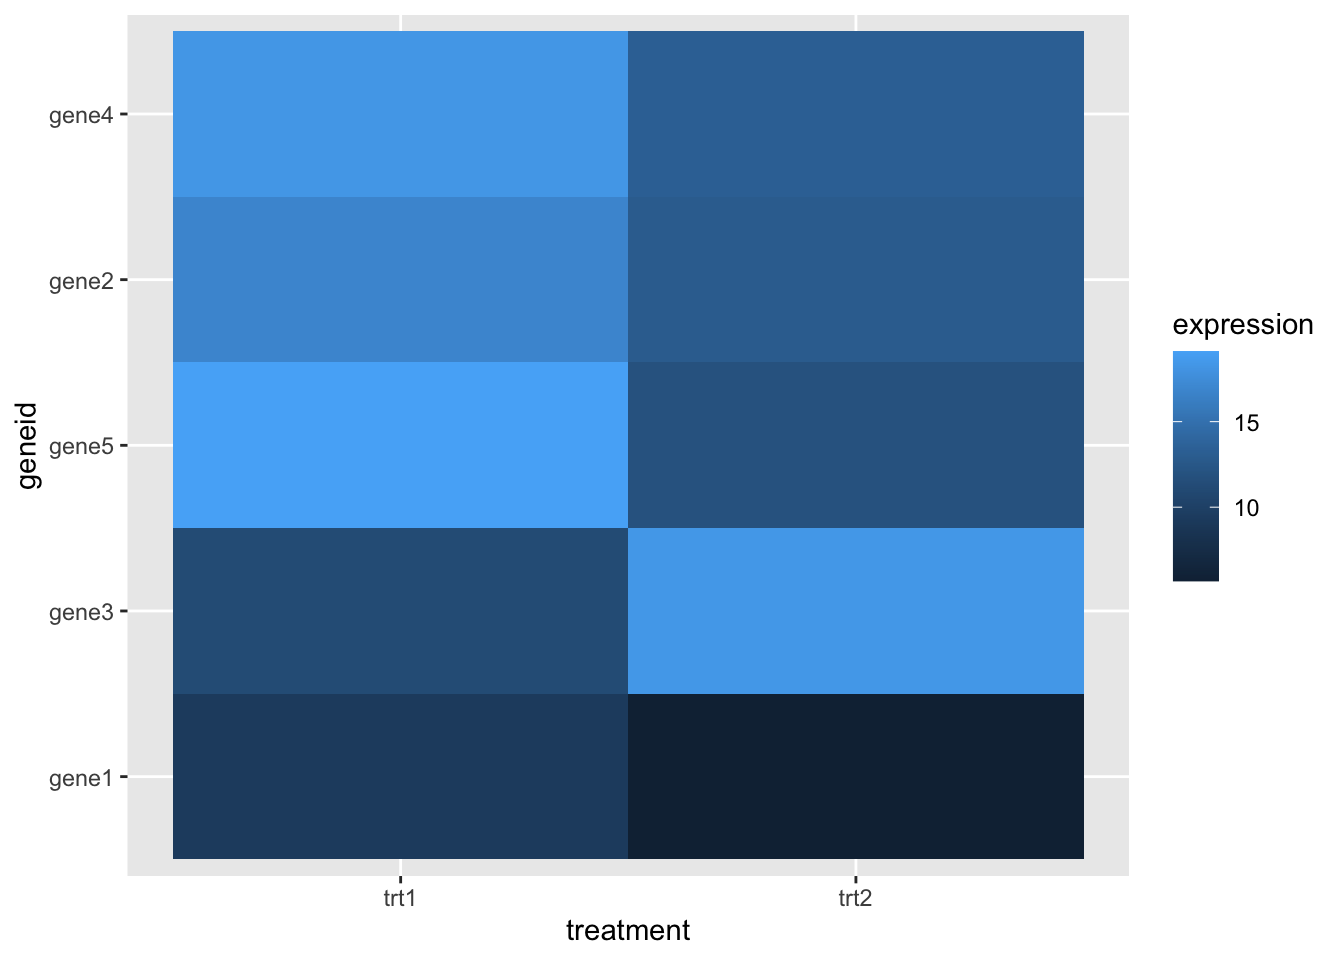
\includegraphics{machine_learning_files/figure-latex/unnamed-chunk-33-1.pdf}

The \texttt{ggdendro} package allows us to create a dendrogram from a clustering

\begin{Shaded}
\begin{Highlighting}[]
\KeywordTok{library}\NormalTok{(ggdendro)}
\NormalTok{dendro <-}\StringTok{ }\KeywordTok{ggdendrogram}\NormalTok{(clusters) }\OperatorTok{+}\StringTok{ }\KeywordTok{coord_flip}\NormalTok{() }\OperatorTok{+}\StringTok{ }\KeywordTok{theme_dendro}\NormalTok{()}
\NormalTok{dendro}
\end{Highlighting}
\end{Shaded}

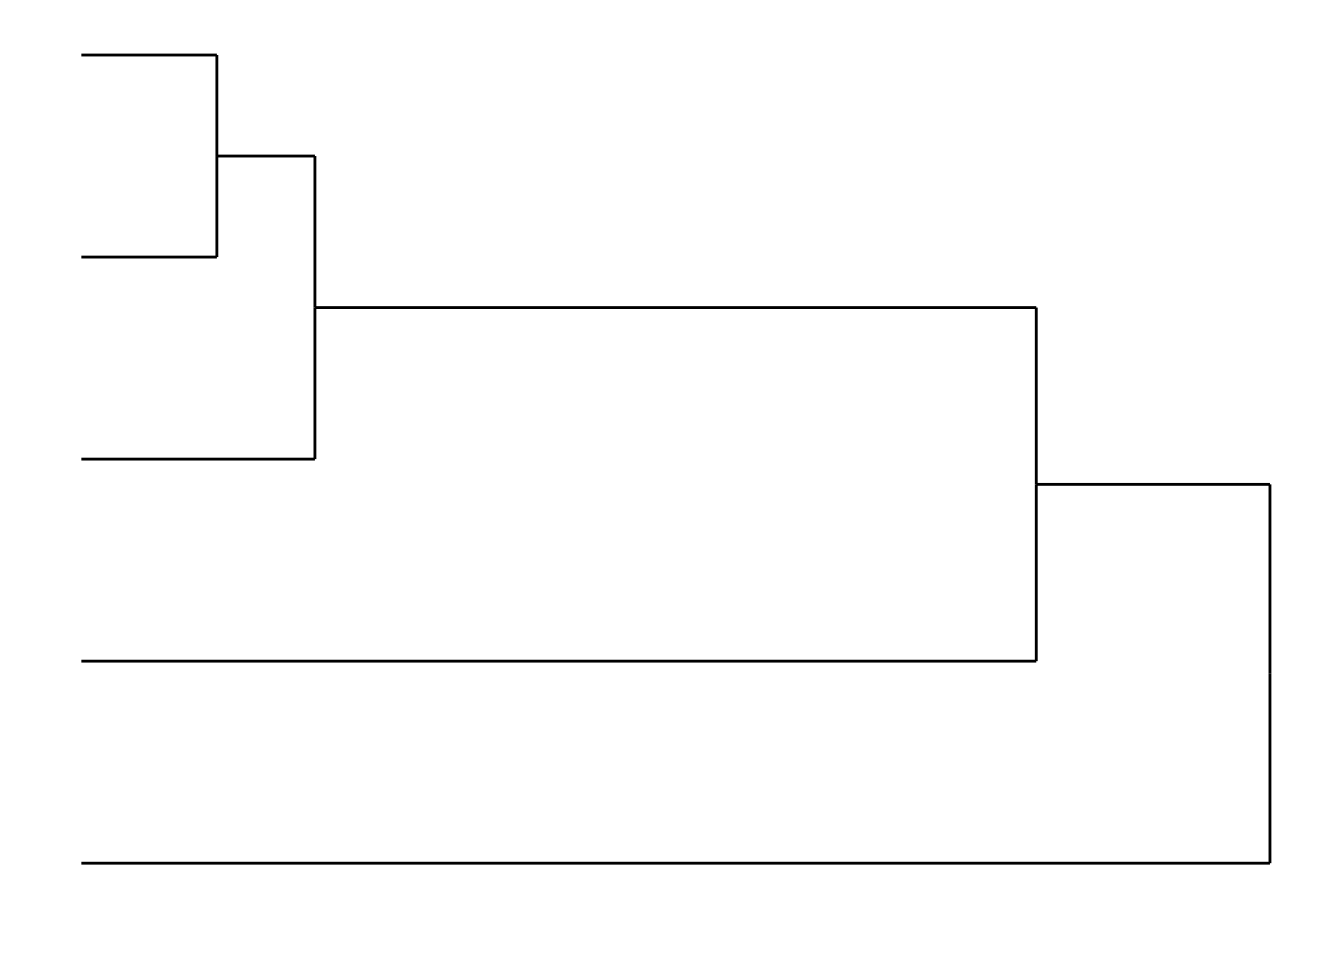
\includegraphics{machine_learning_files/figure-latex/unnamed-chunk-34-1.pdf}

We can compose the two plots with \texttt{patchwork} (cheekily moving the legend out of the way first).

\begin{Shaded}
\begin{Highlighting}[]
\KeywordTok{library}\NormalTok{(patchwork)}
\NormalTok{hmap }\OperatorTok{+}\StringTok{ }\KeywordTok{theme}\NormalTok{(}\DataTypeTok{legend.position=}\StringTok{"bottom"}\NormalTok{) }\OperatorTok{+}\StringTok{  }\NormalTok{dendro}
\end{Highlighting}
\end{Shaded}

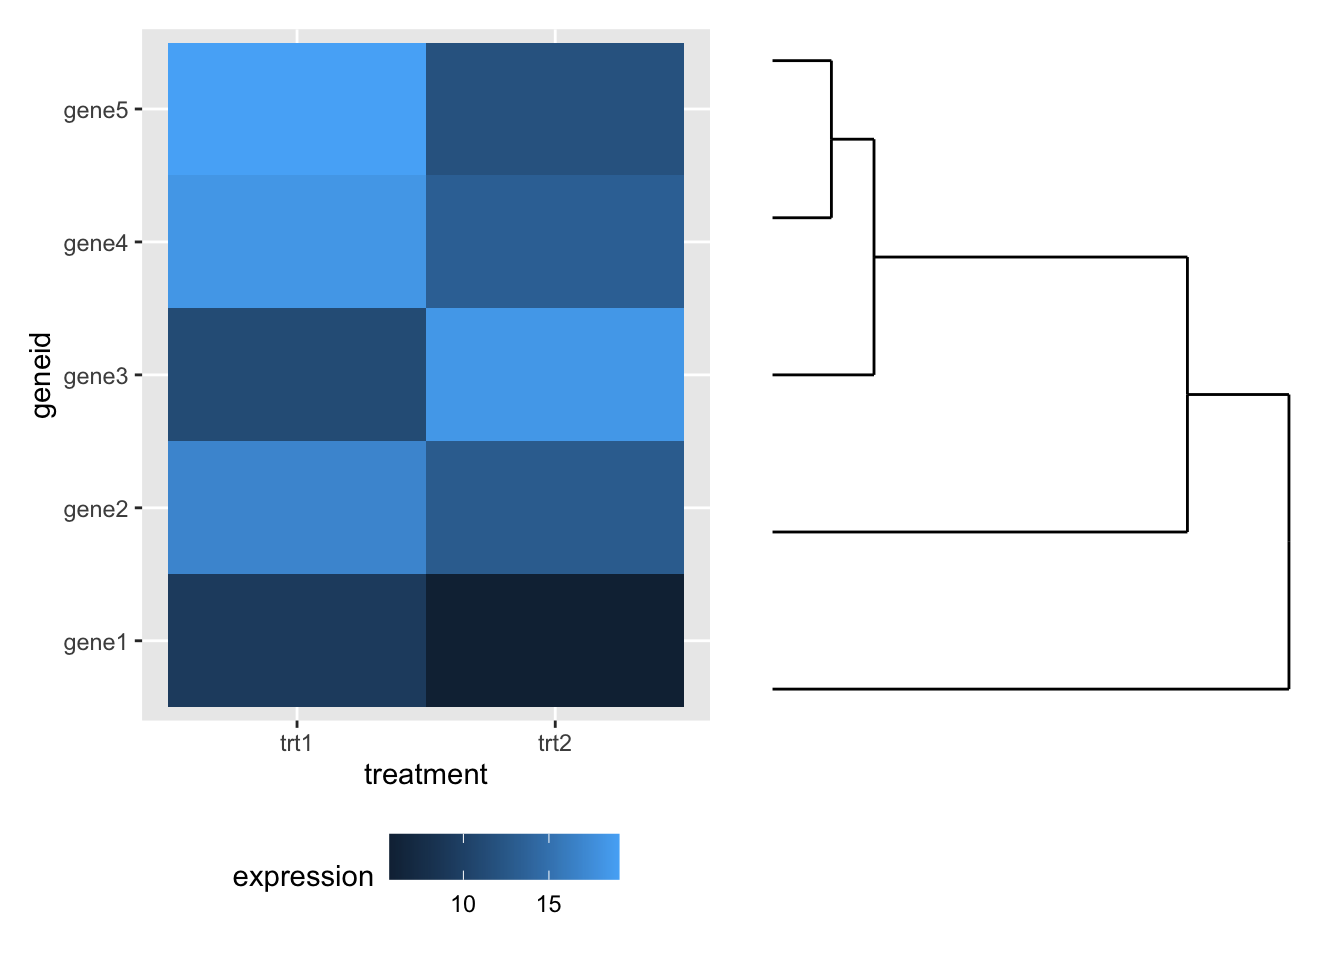
\includegraphics{machine_learning_files/figure-latex/unnamed-chunk-35-1.pdf}

\hypertarget{k-means-clustering}{%
\section{K-Means clustering}\label{k-means-clustering}}

A limitation of hierarchical clustering is that we as the operator have to guess what elements are in which cluster and that can be a bit arbitrary. An alternative algorithm, the K-means cluster gets around this problem by allowing us to specify the number of clusters up-front and works from there. It starts with the assumption that there are \texttt{k} clusters and makes \texttt{k} random cluster start points (centroids) then tries to assign cases (elements/observations) to one of each centroid based on the distance from the start points. The assignment to clusters is improved iteratively by starting again with the centroid at the mean point in each cluster and continues until no improvements are made. Again, Allison Horst has drawn some great guides

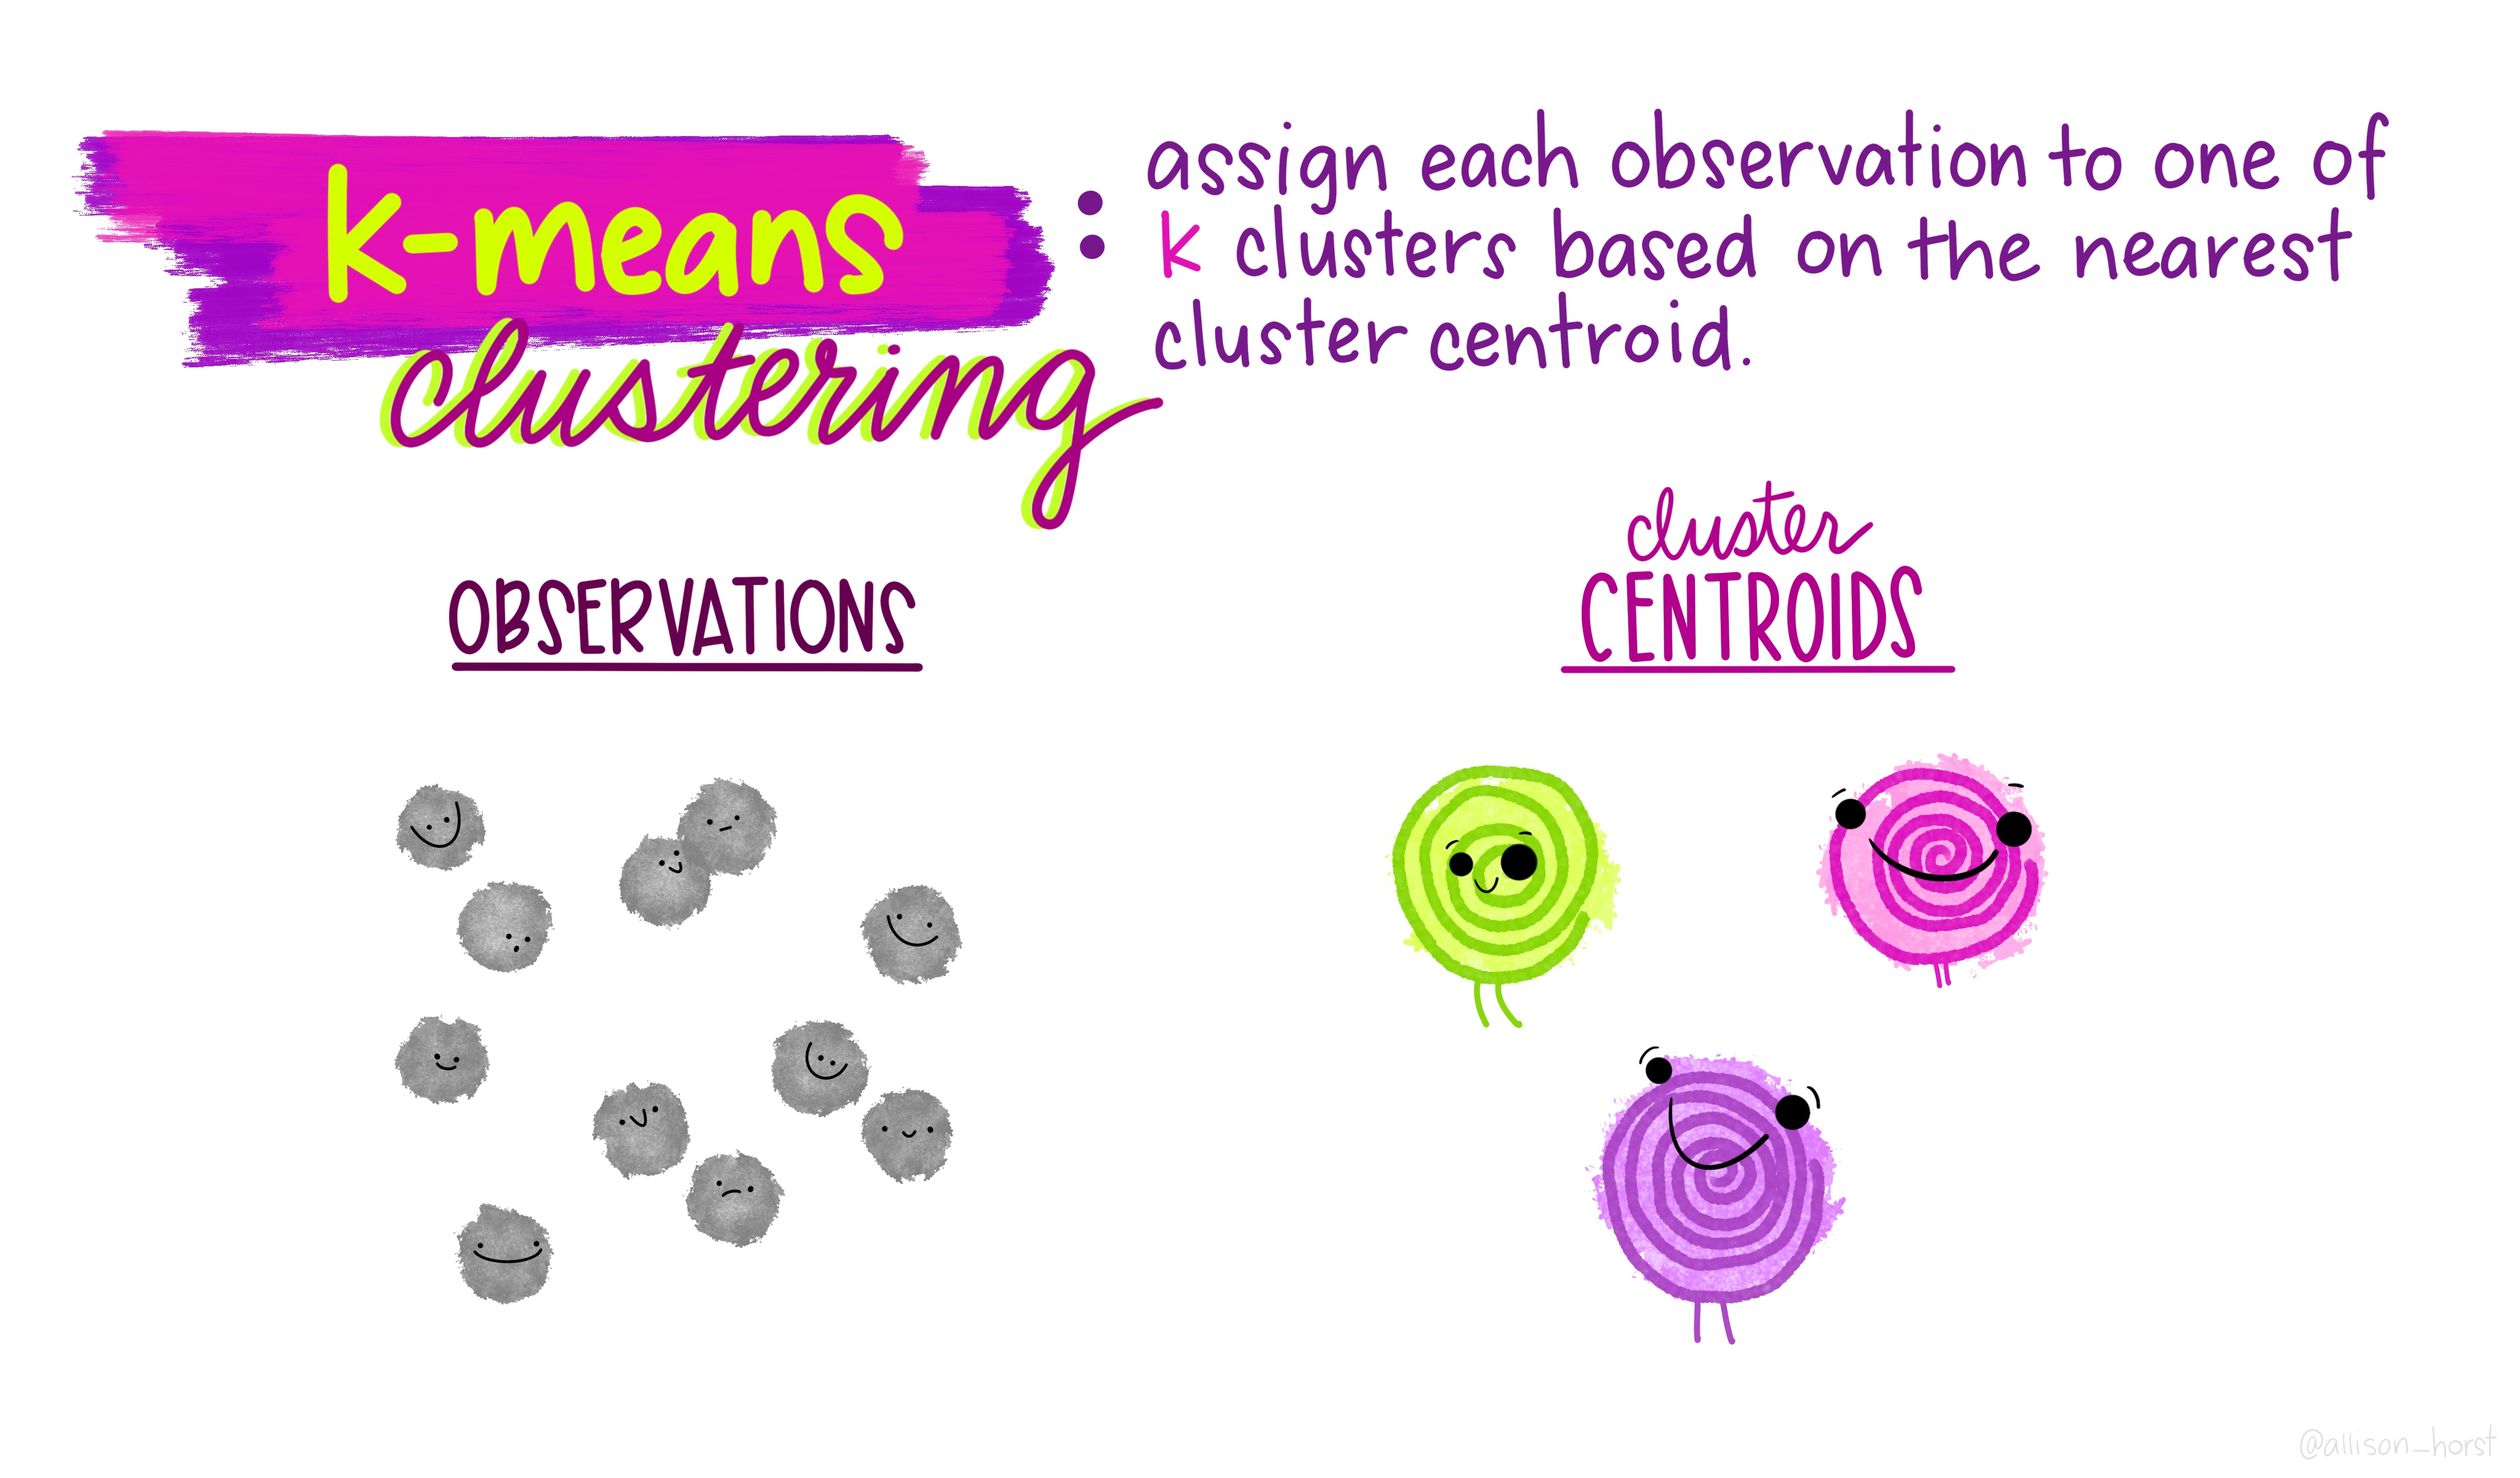
\includegraphics{figs/kmeans_1.jpg} 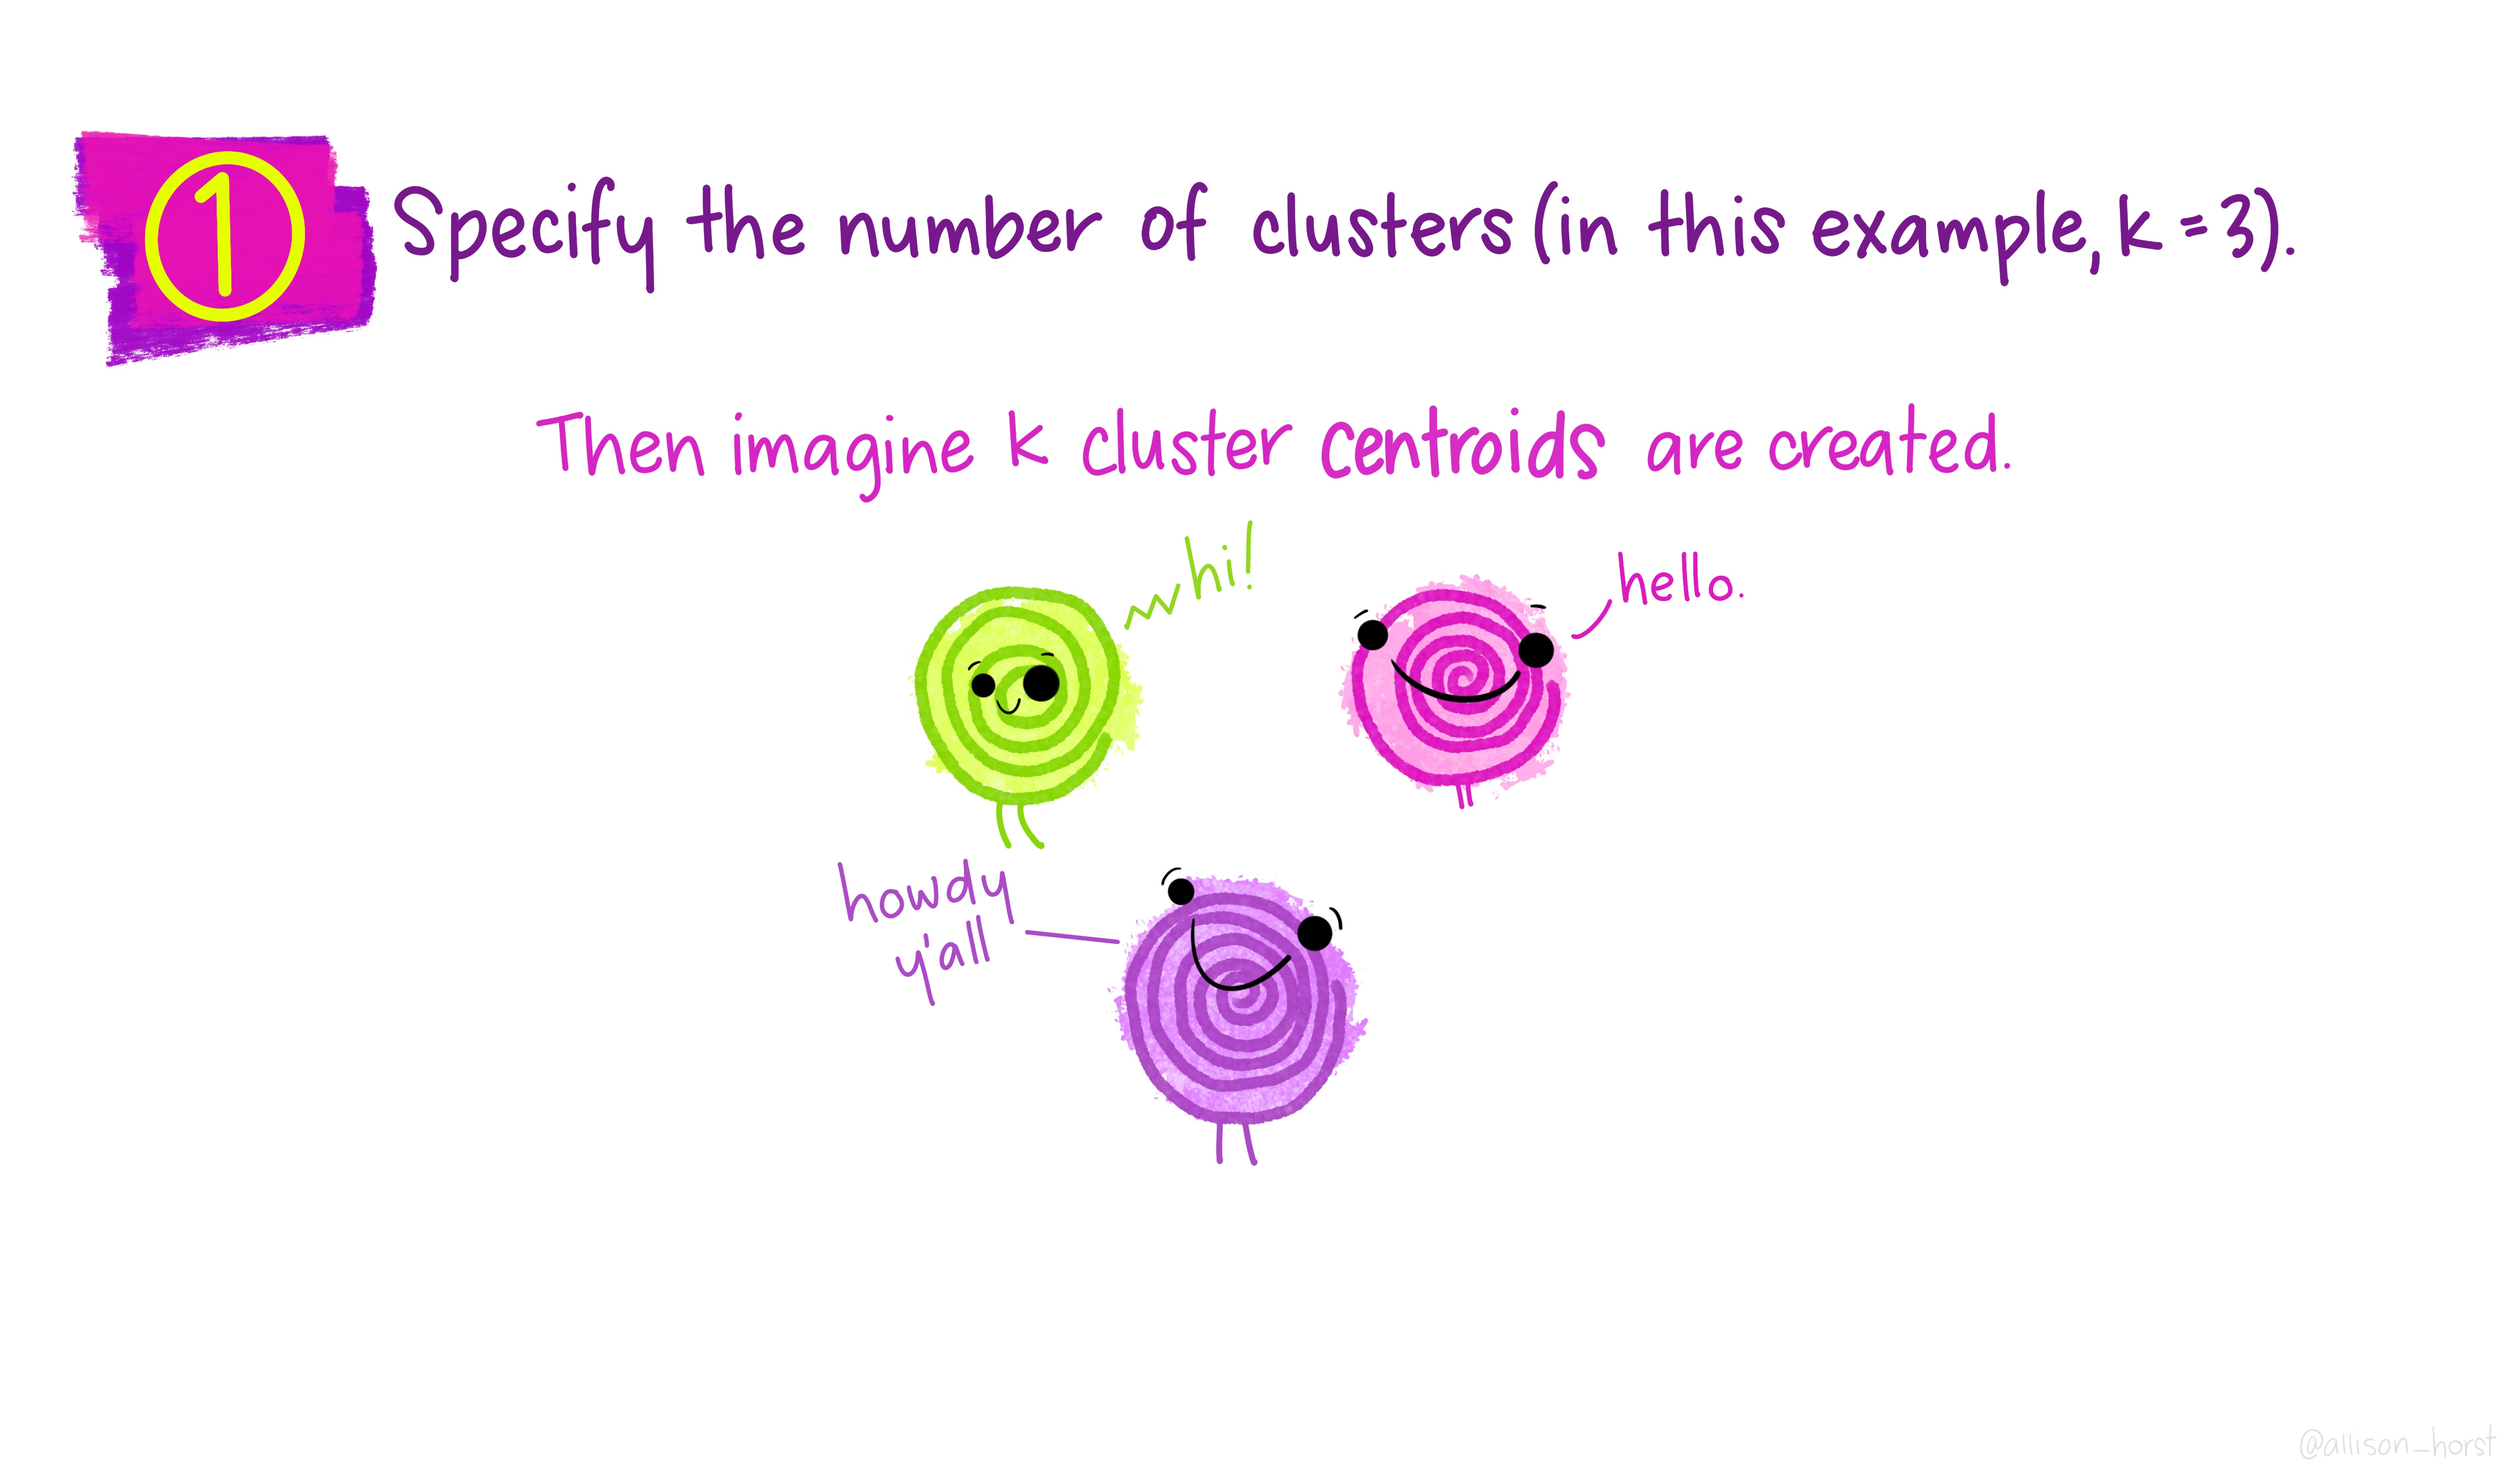
\includegraphics{figs/kmeans_2.jpg} 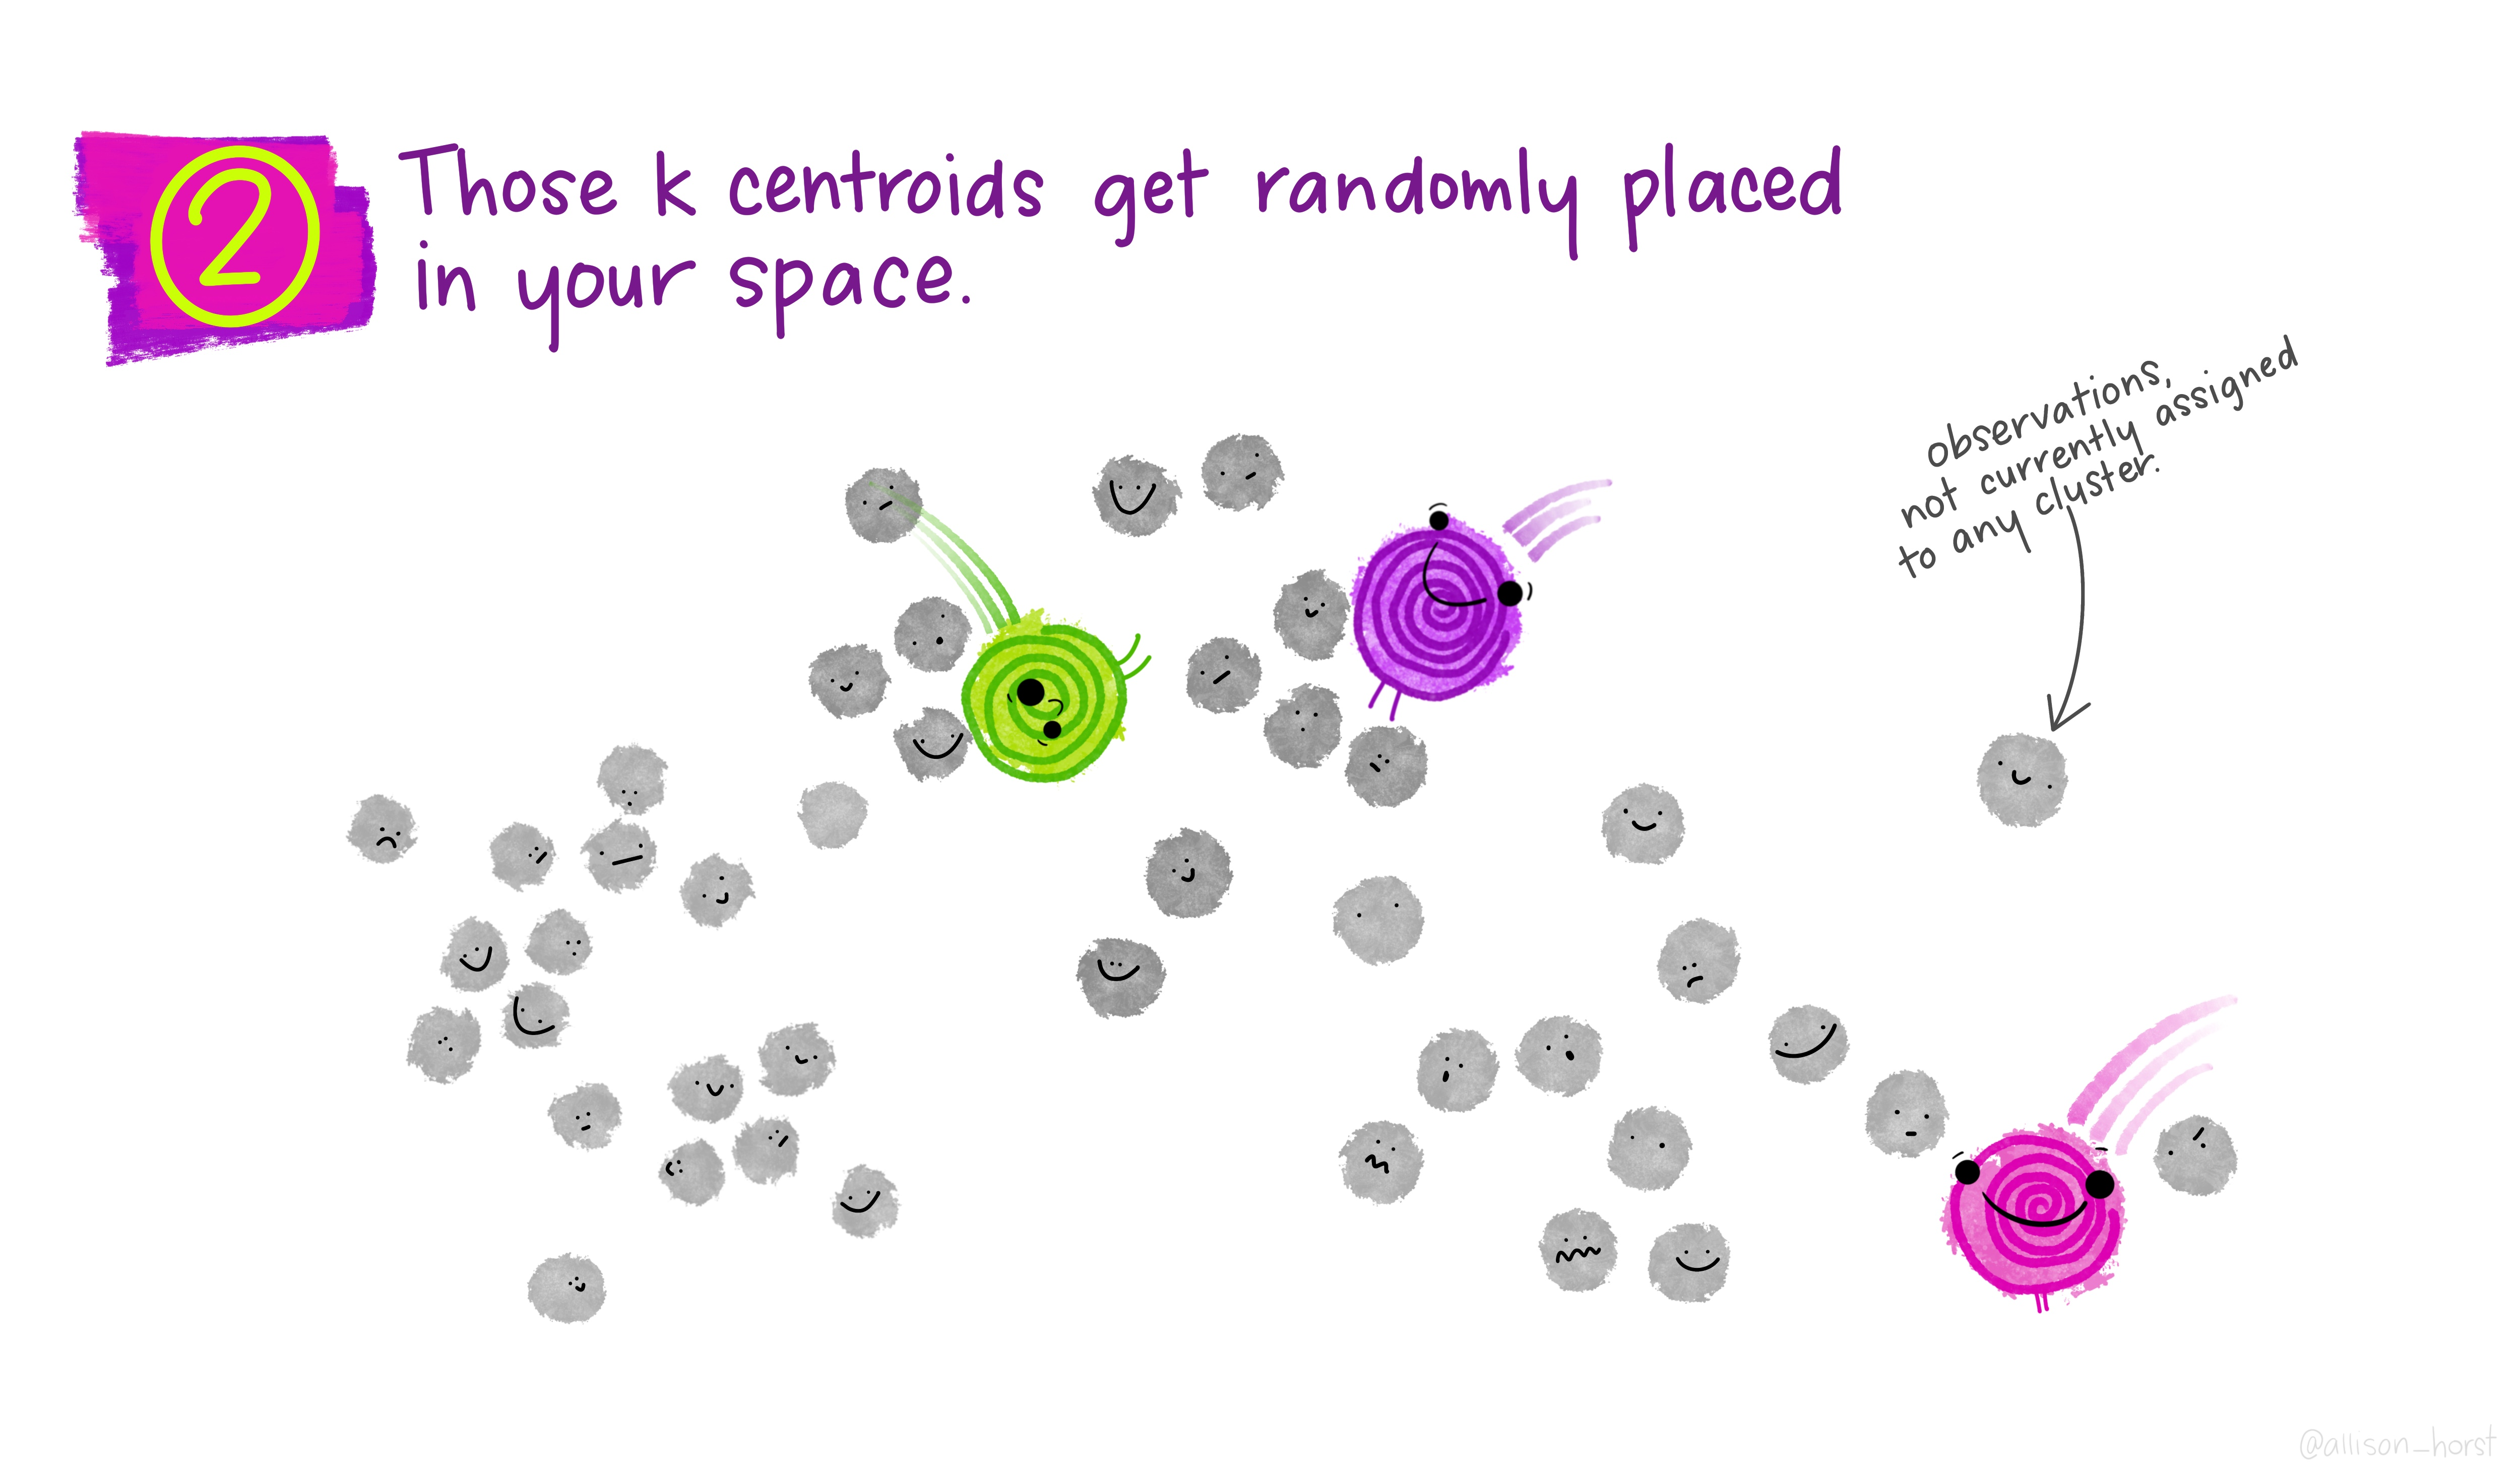
\includegraphics{figs/kmeans_3.jpg} 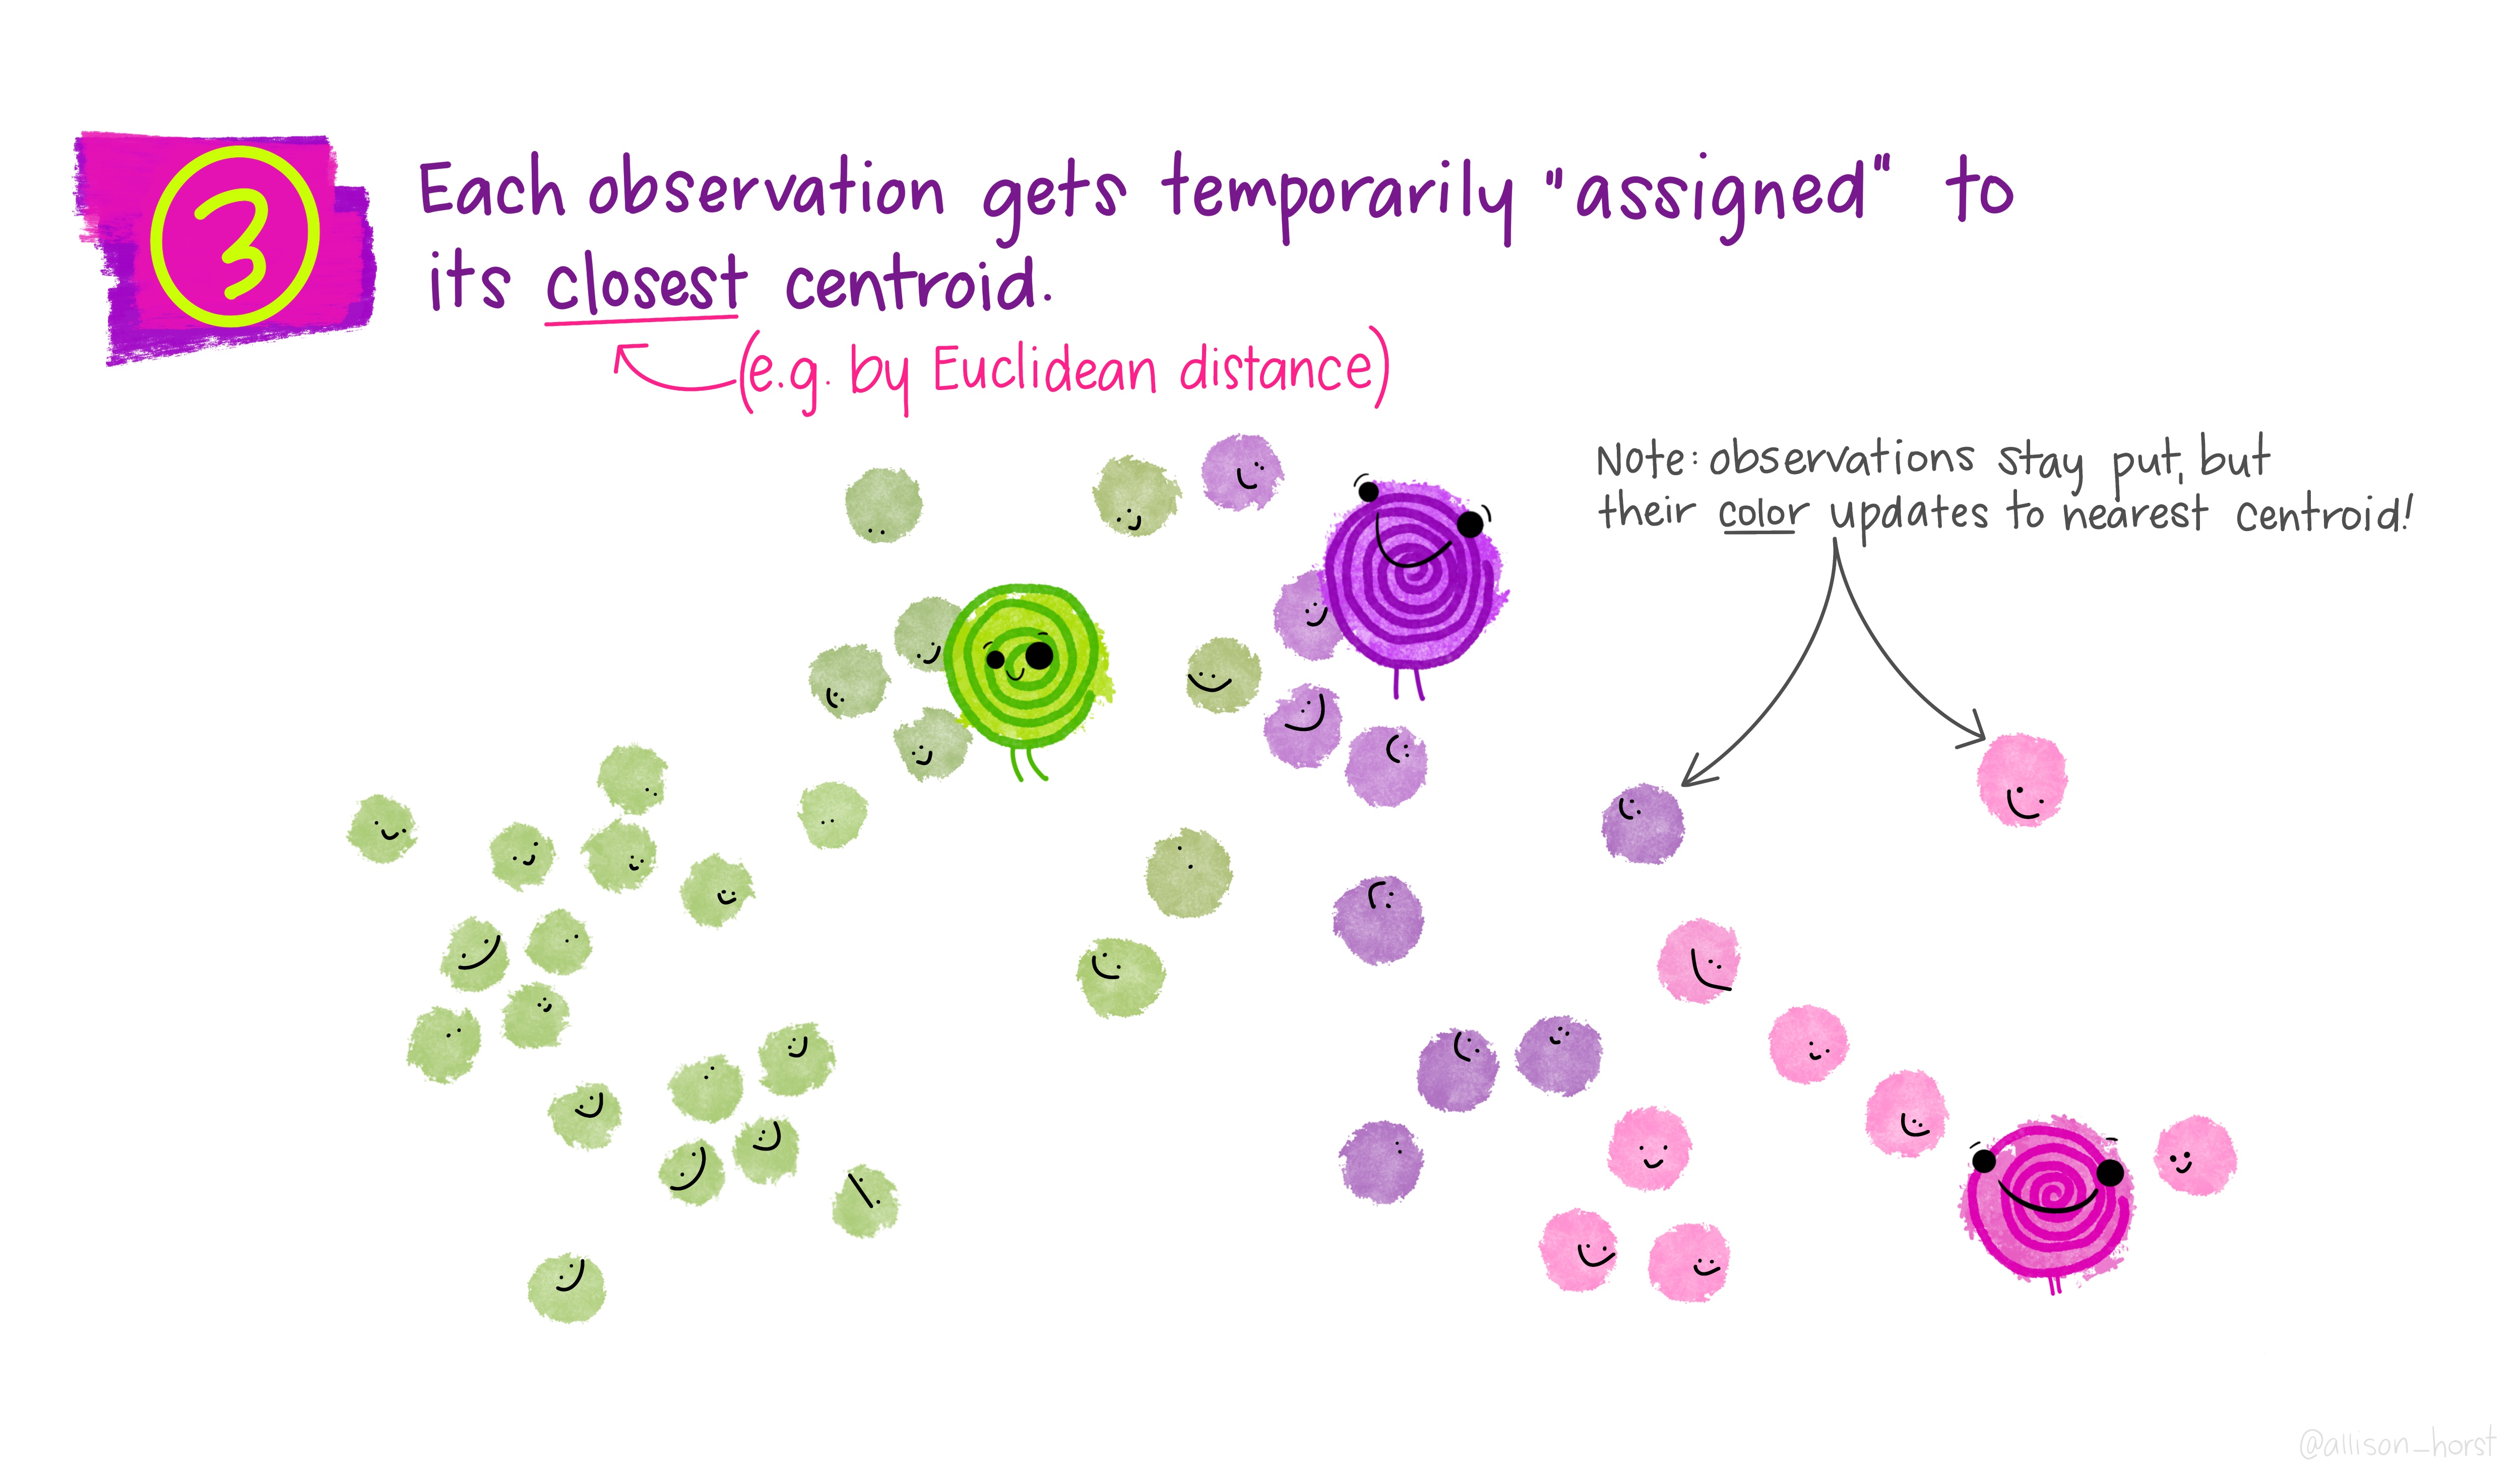
\includegraphics{figs/kmeans_4.jpg} 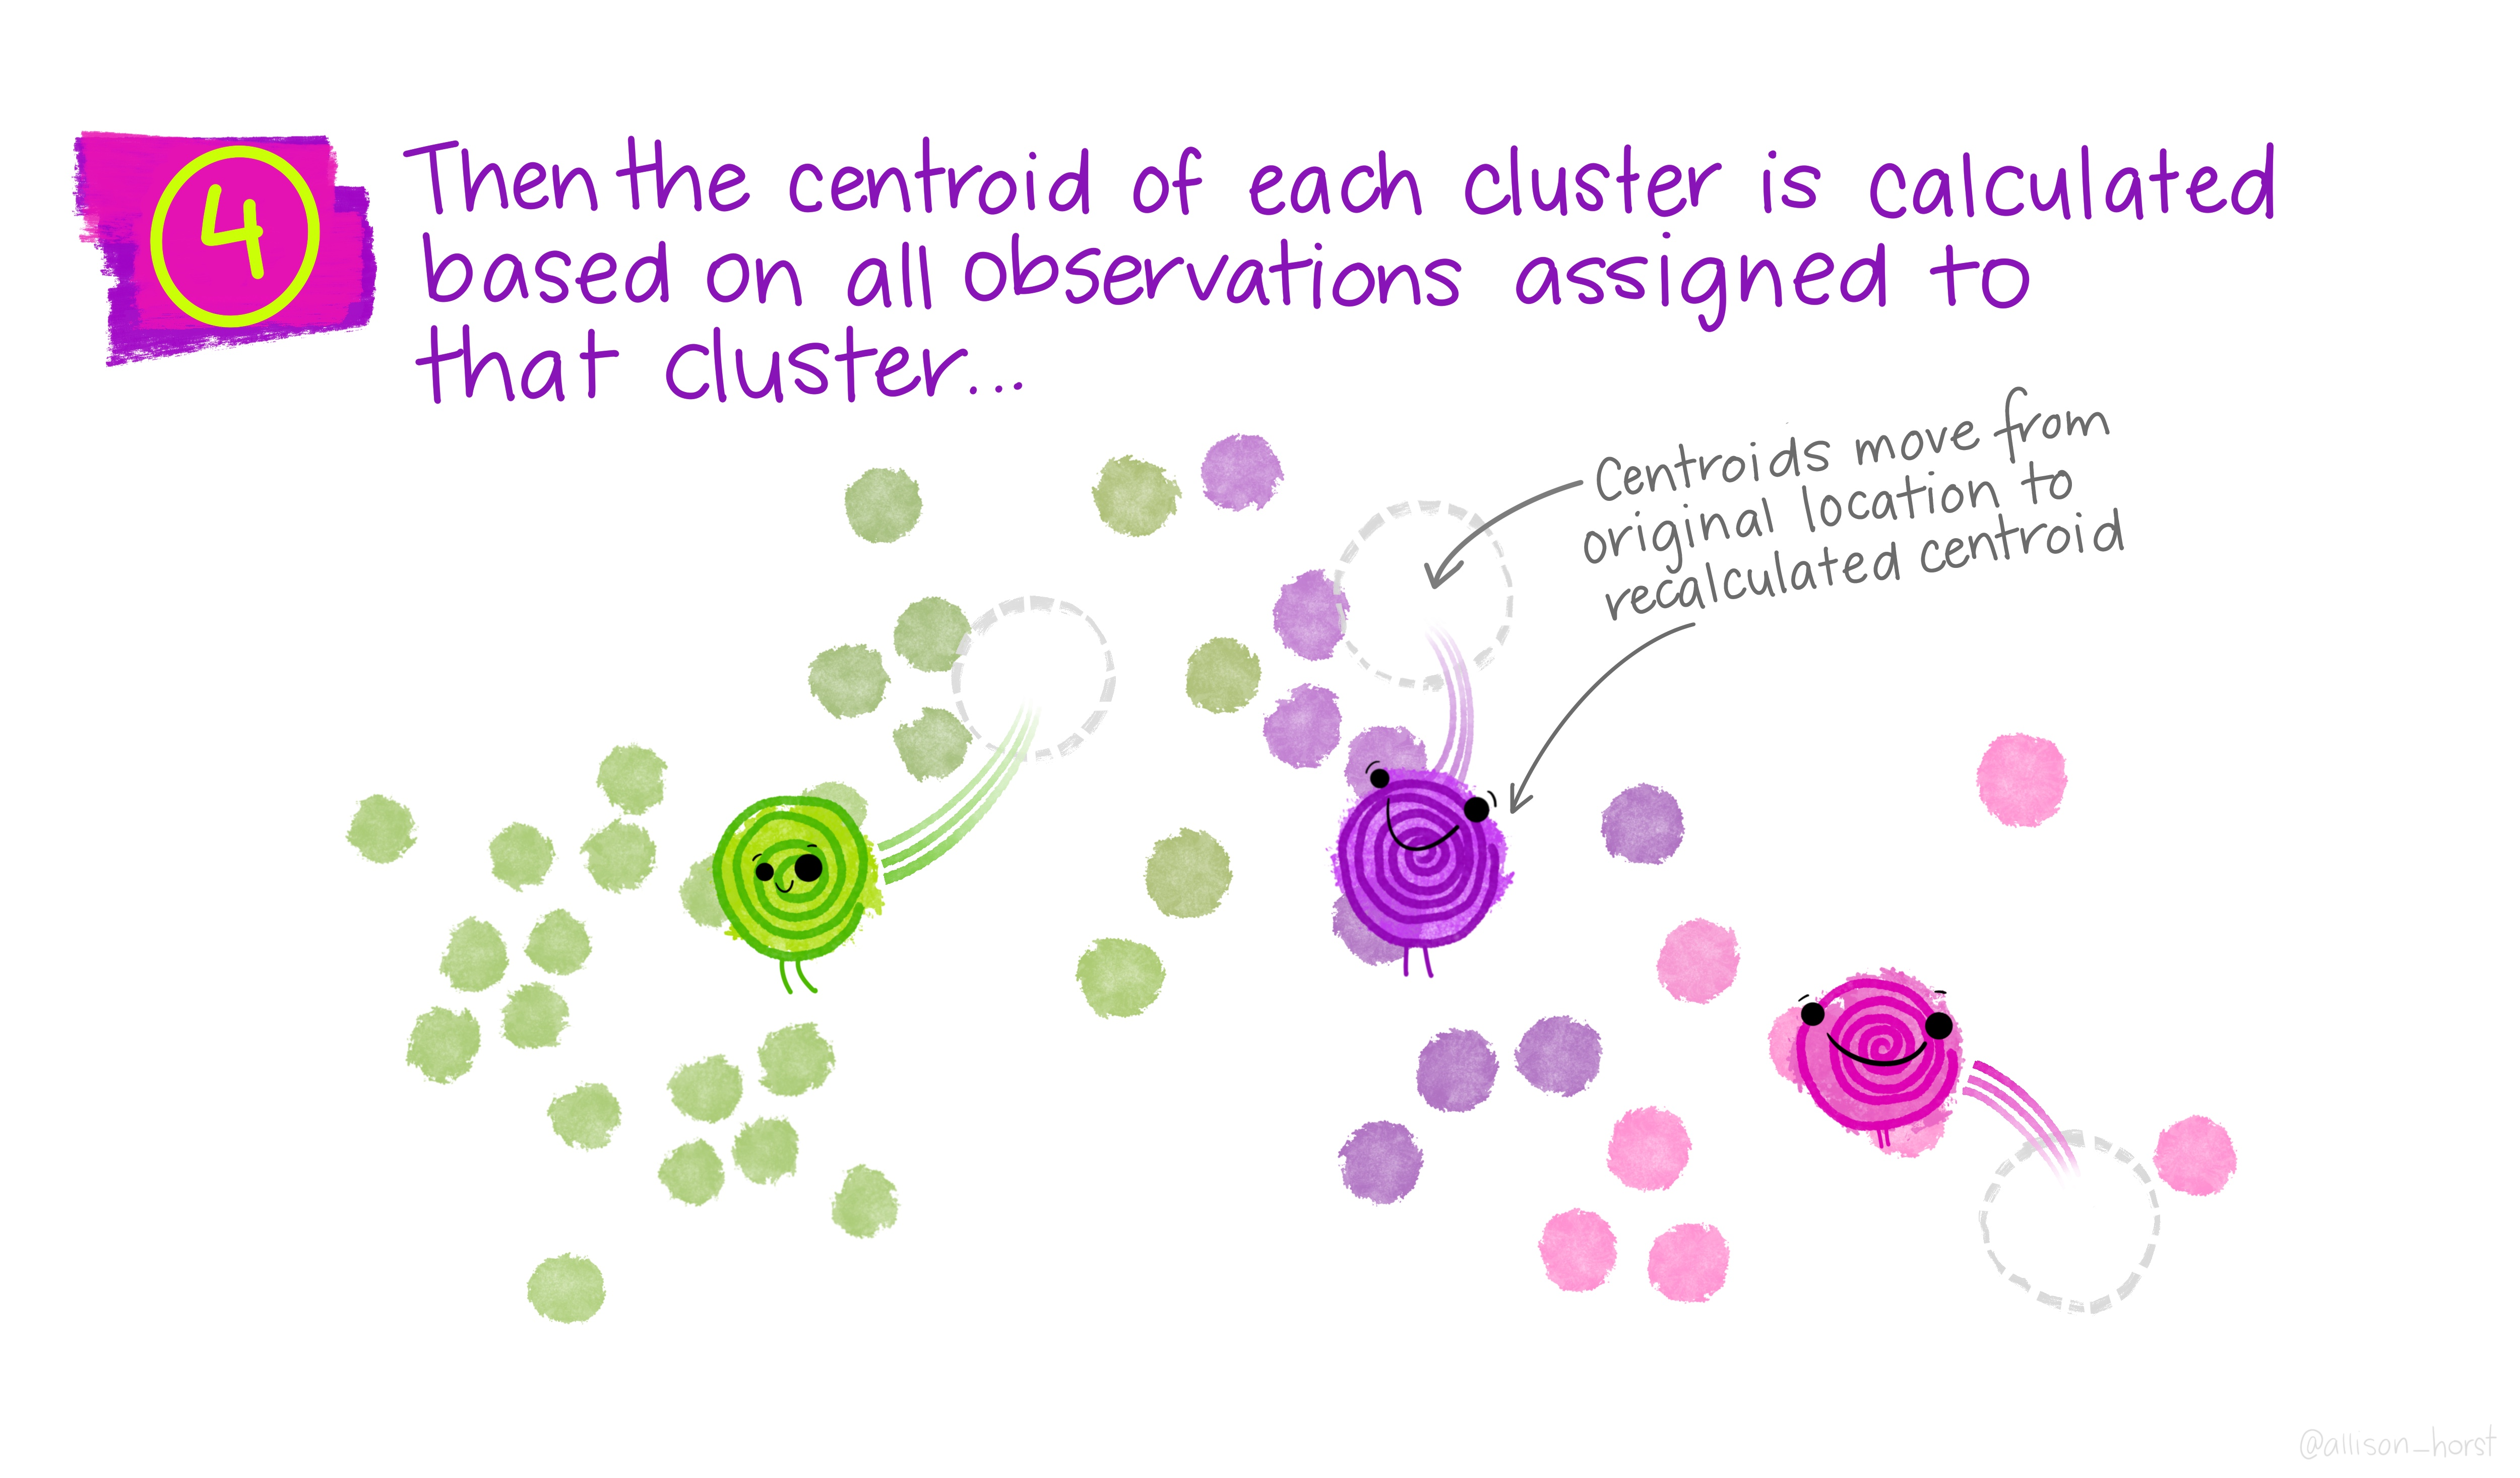
\includegraphics{figs/kmeans_5.jpg} 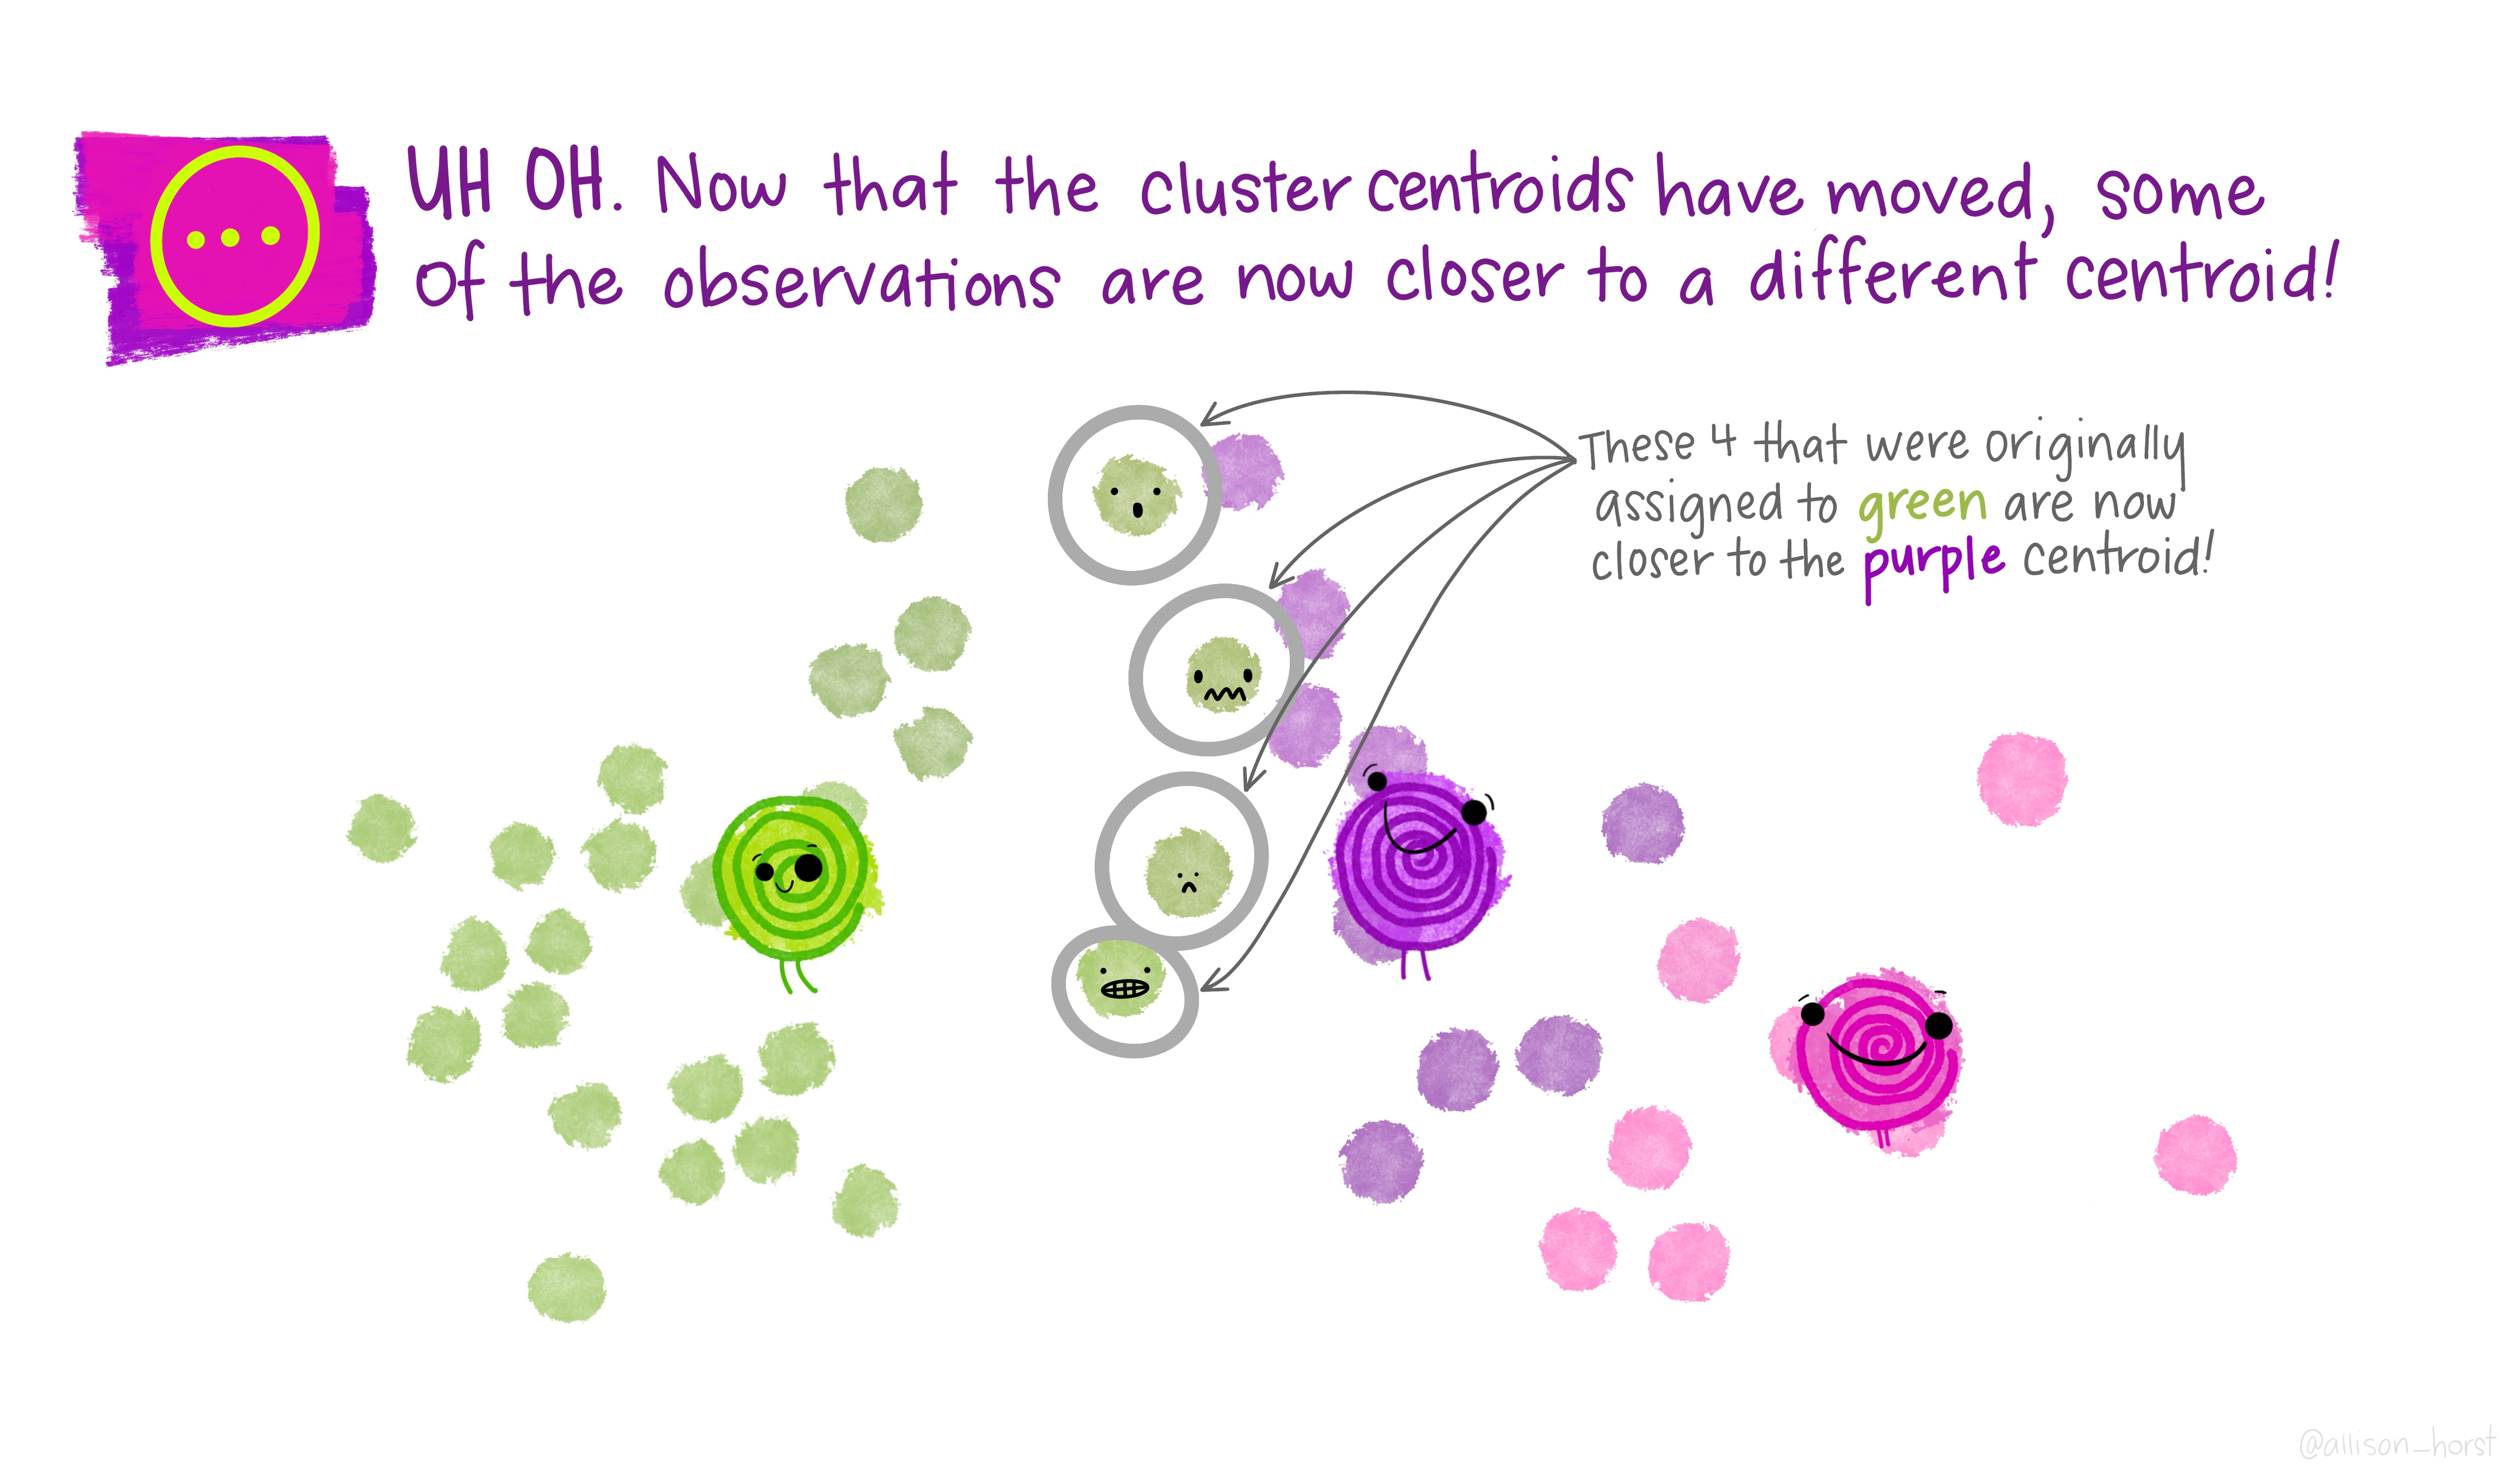
\includegraphics{figs/kmeans_6.jpg} 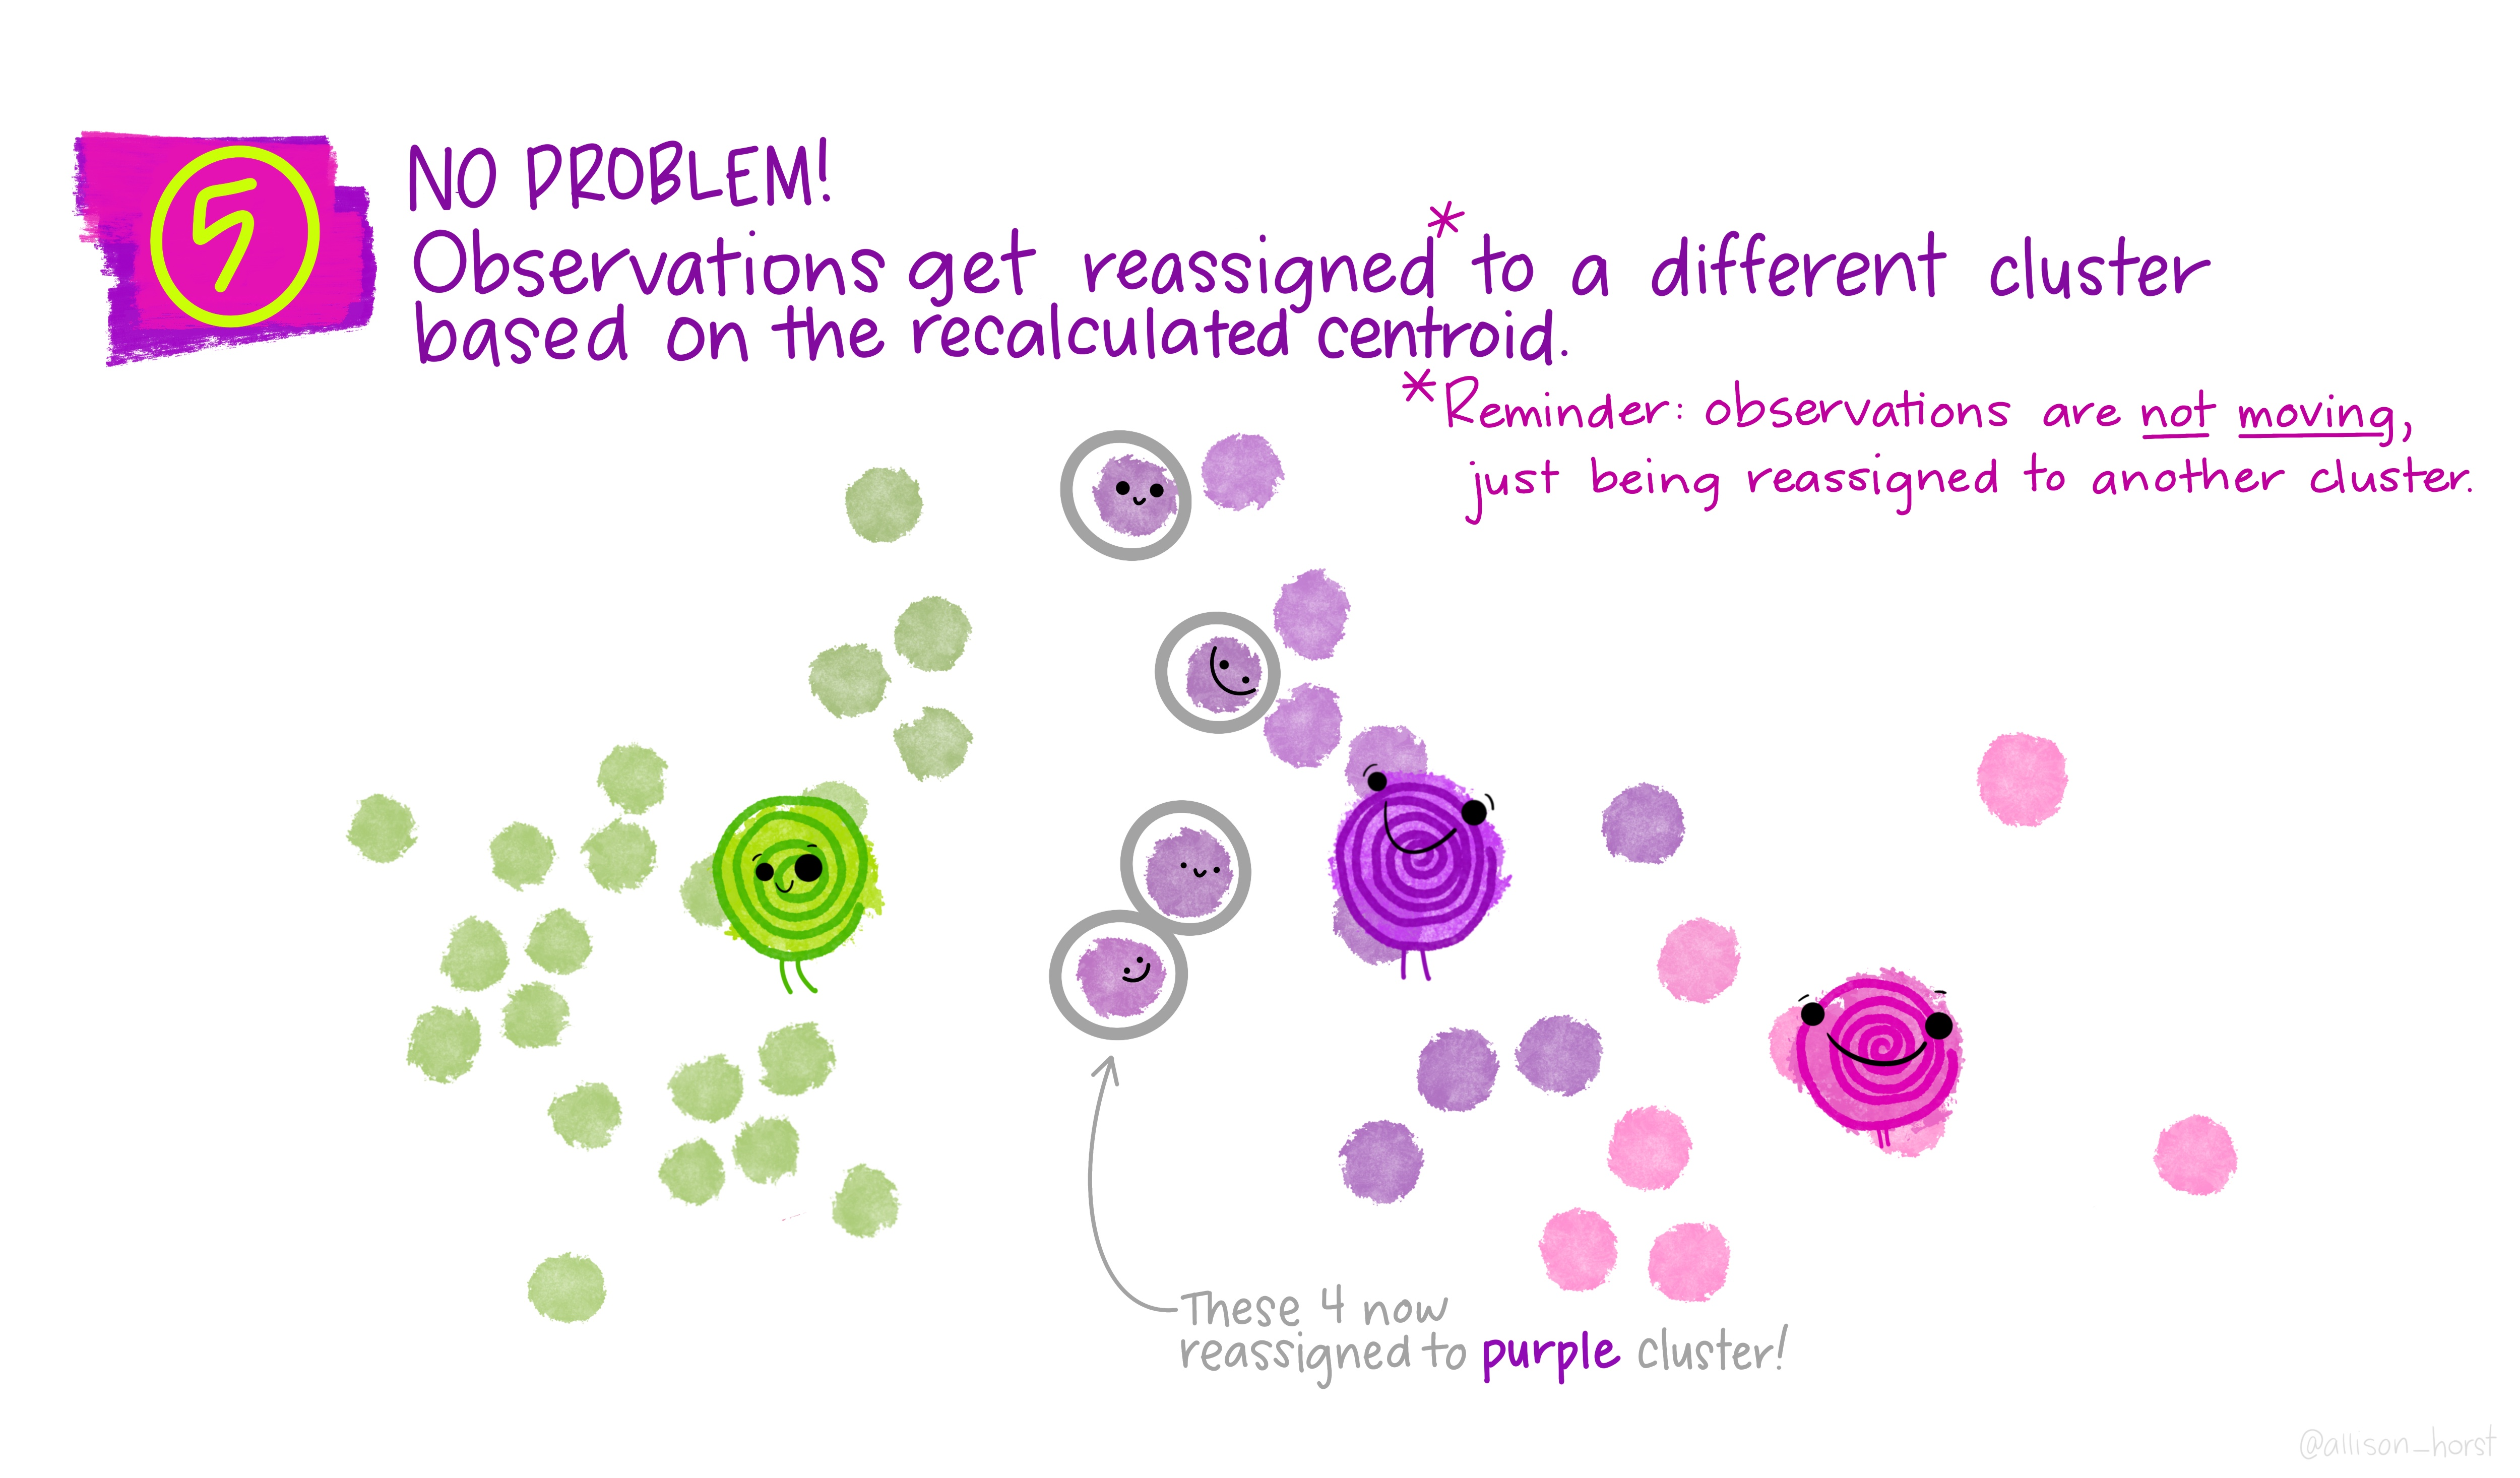
\includegraphics{figs/kmeans_7.jpg} 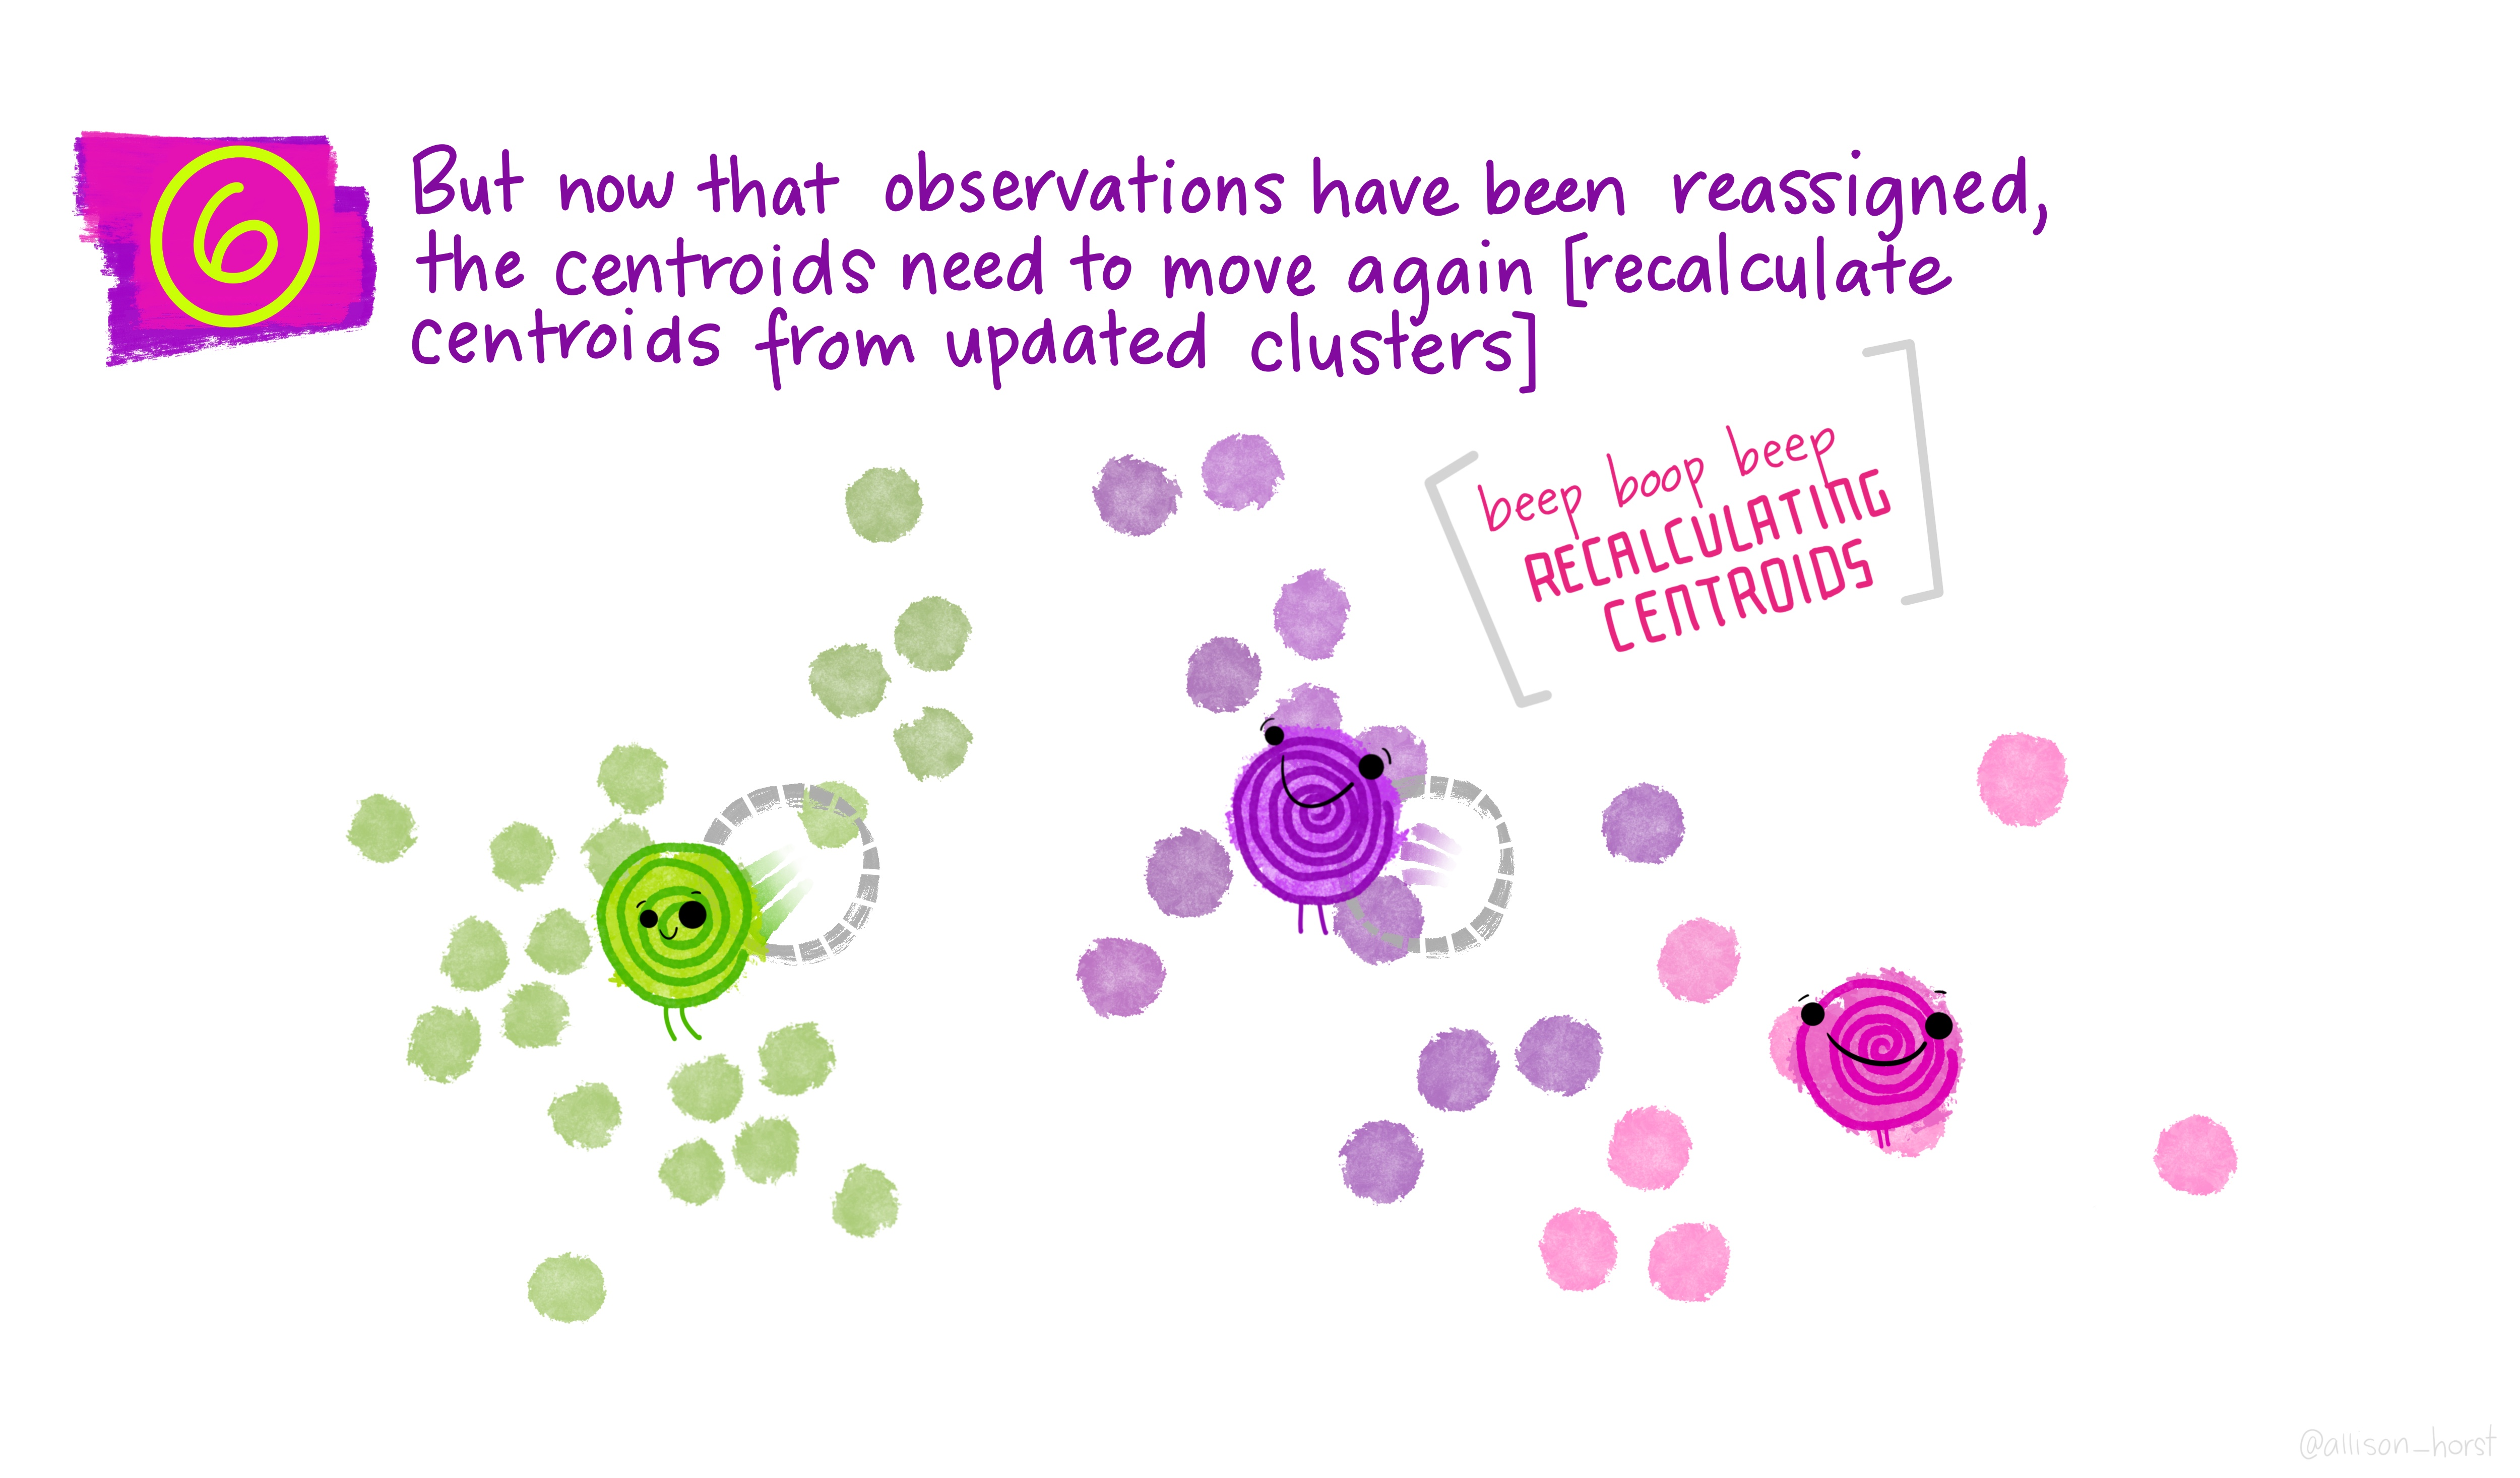
\includegraphics{figs/kmeans_8.jpg} 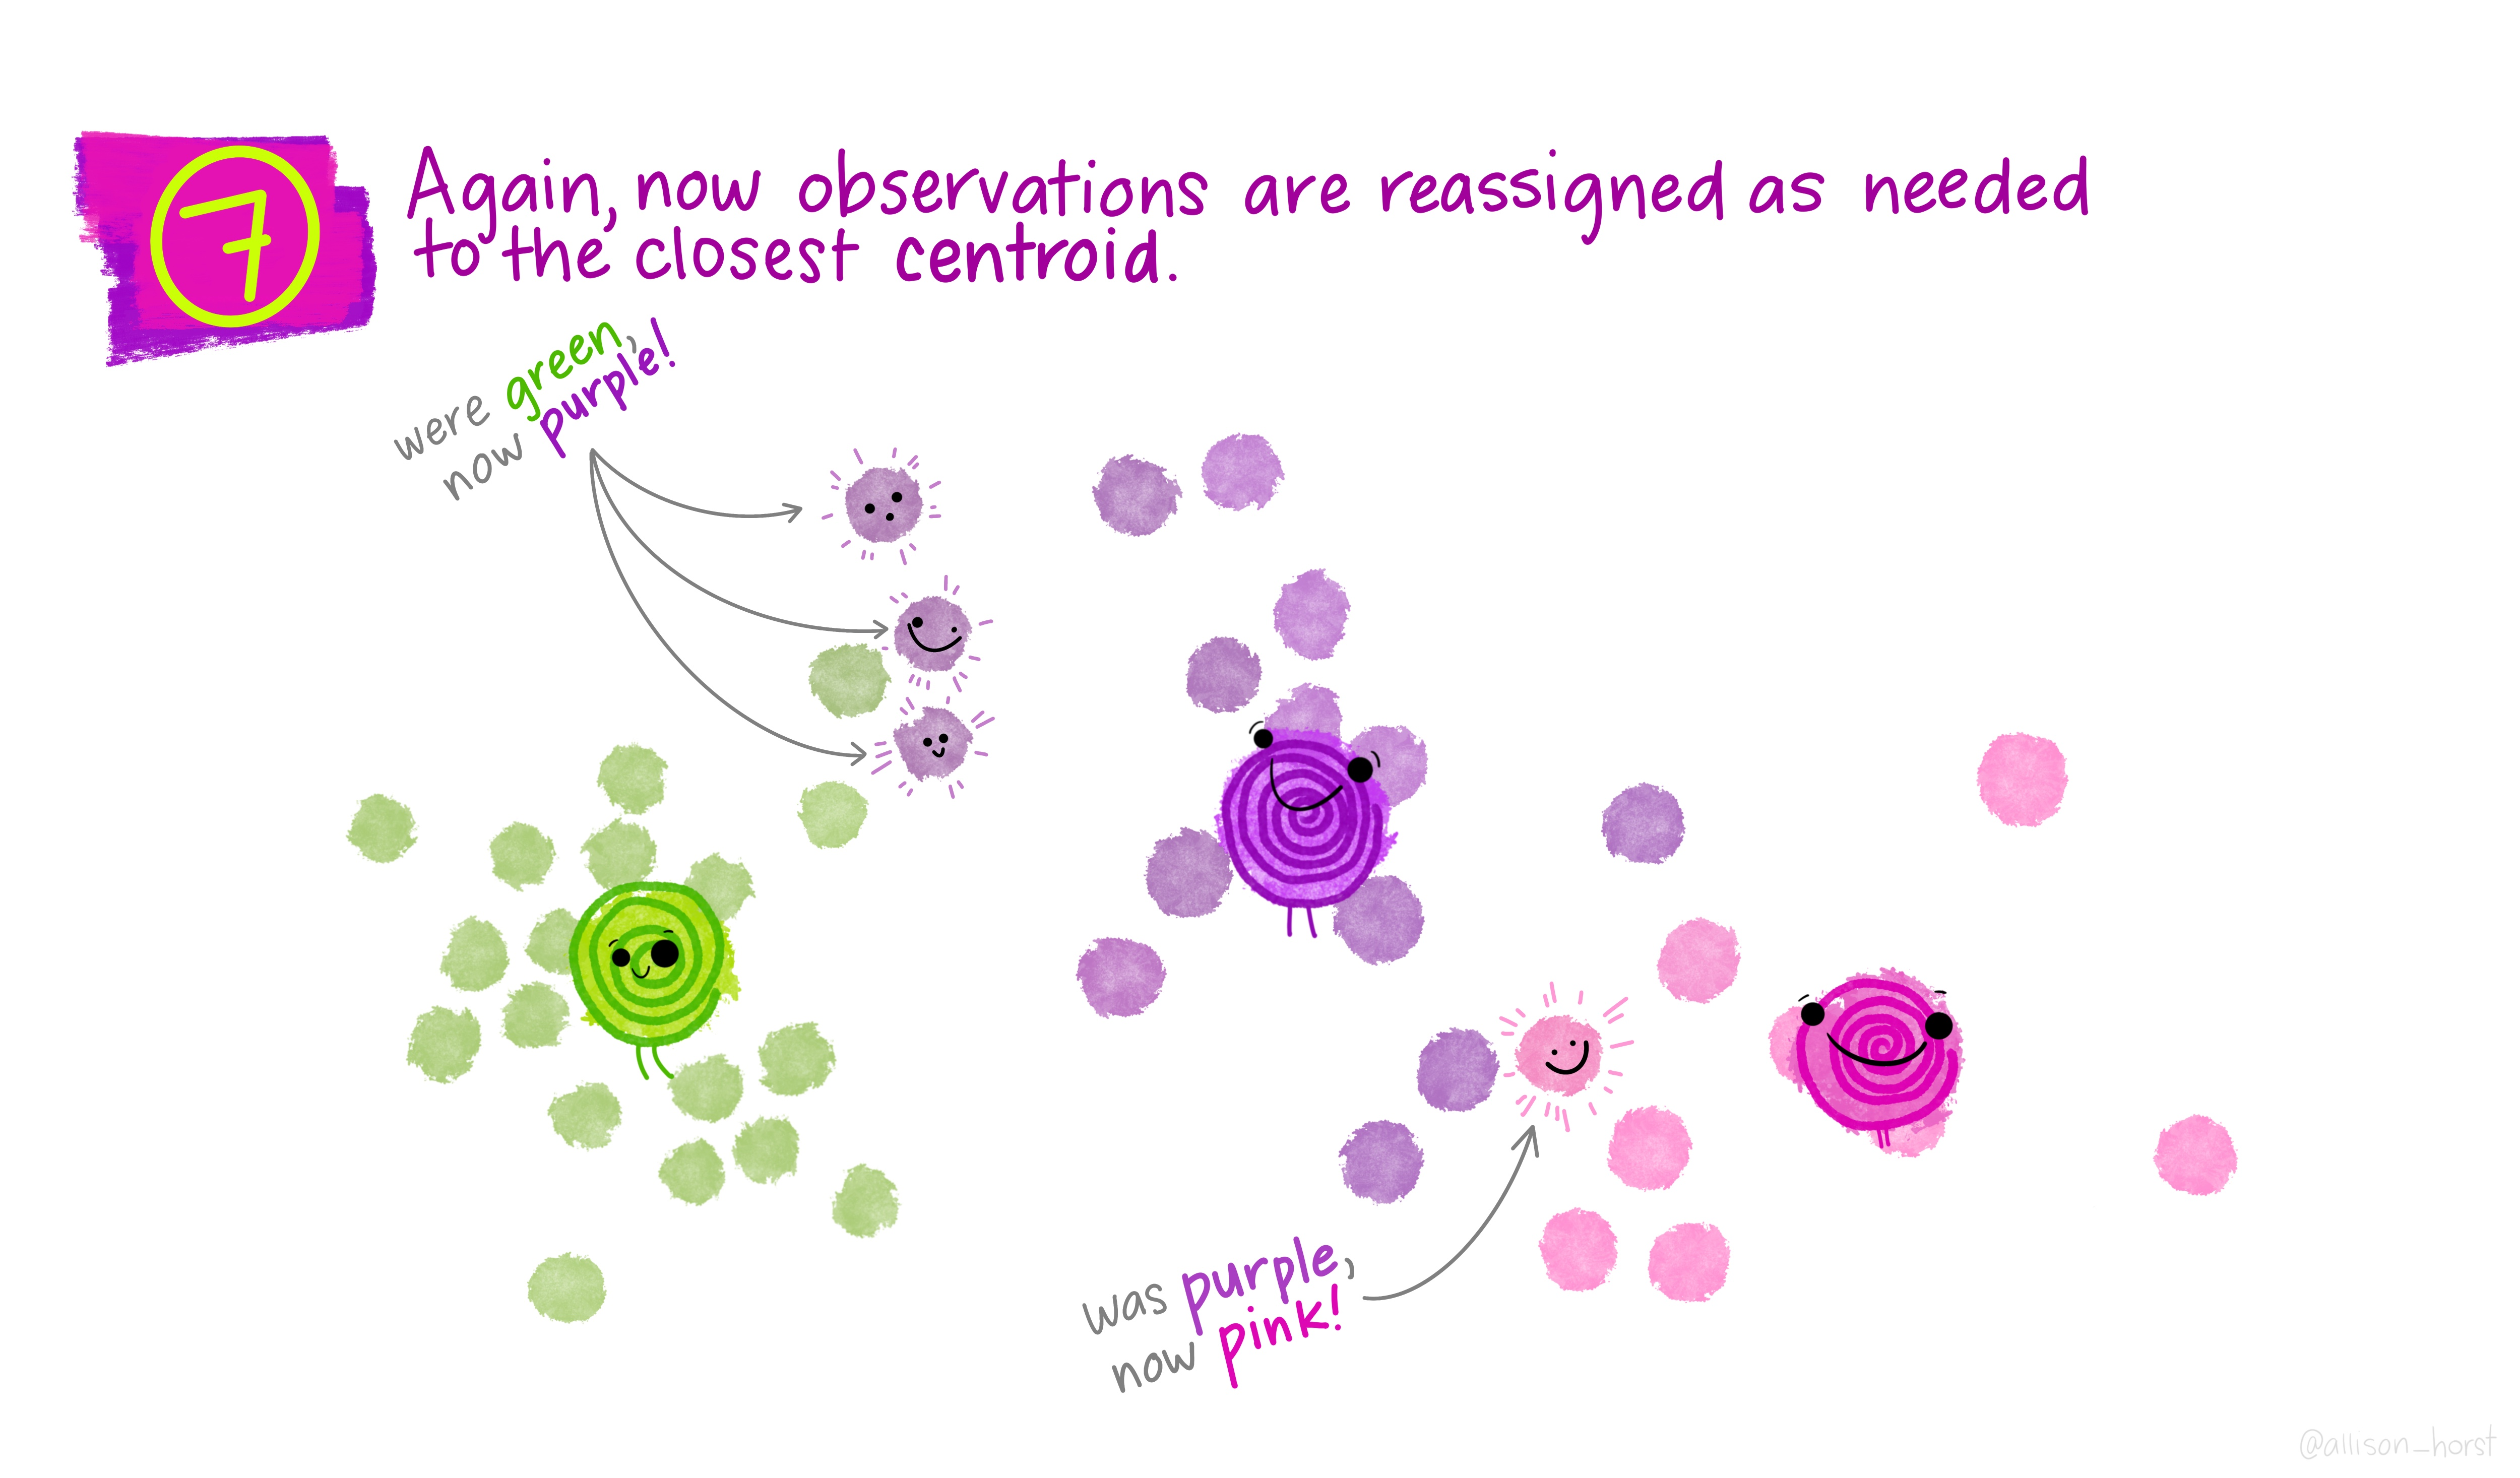
\includegraphics{figs/kmeans_9.jpg} 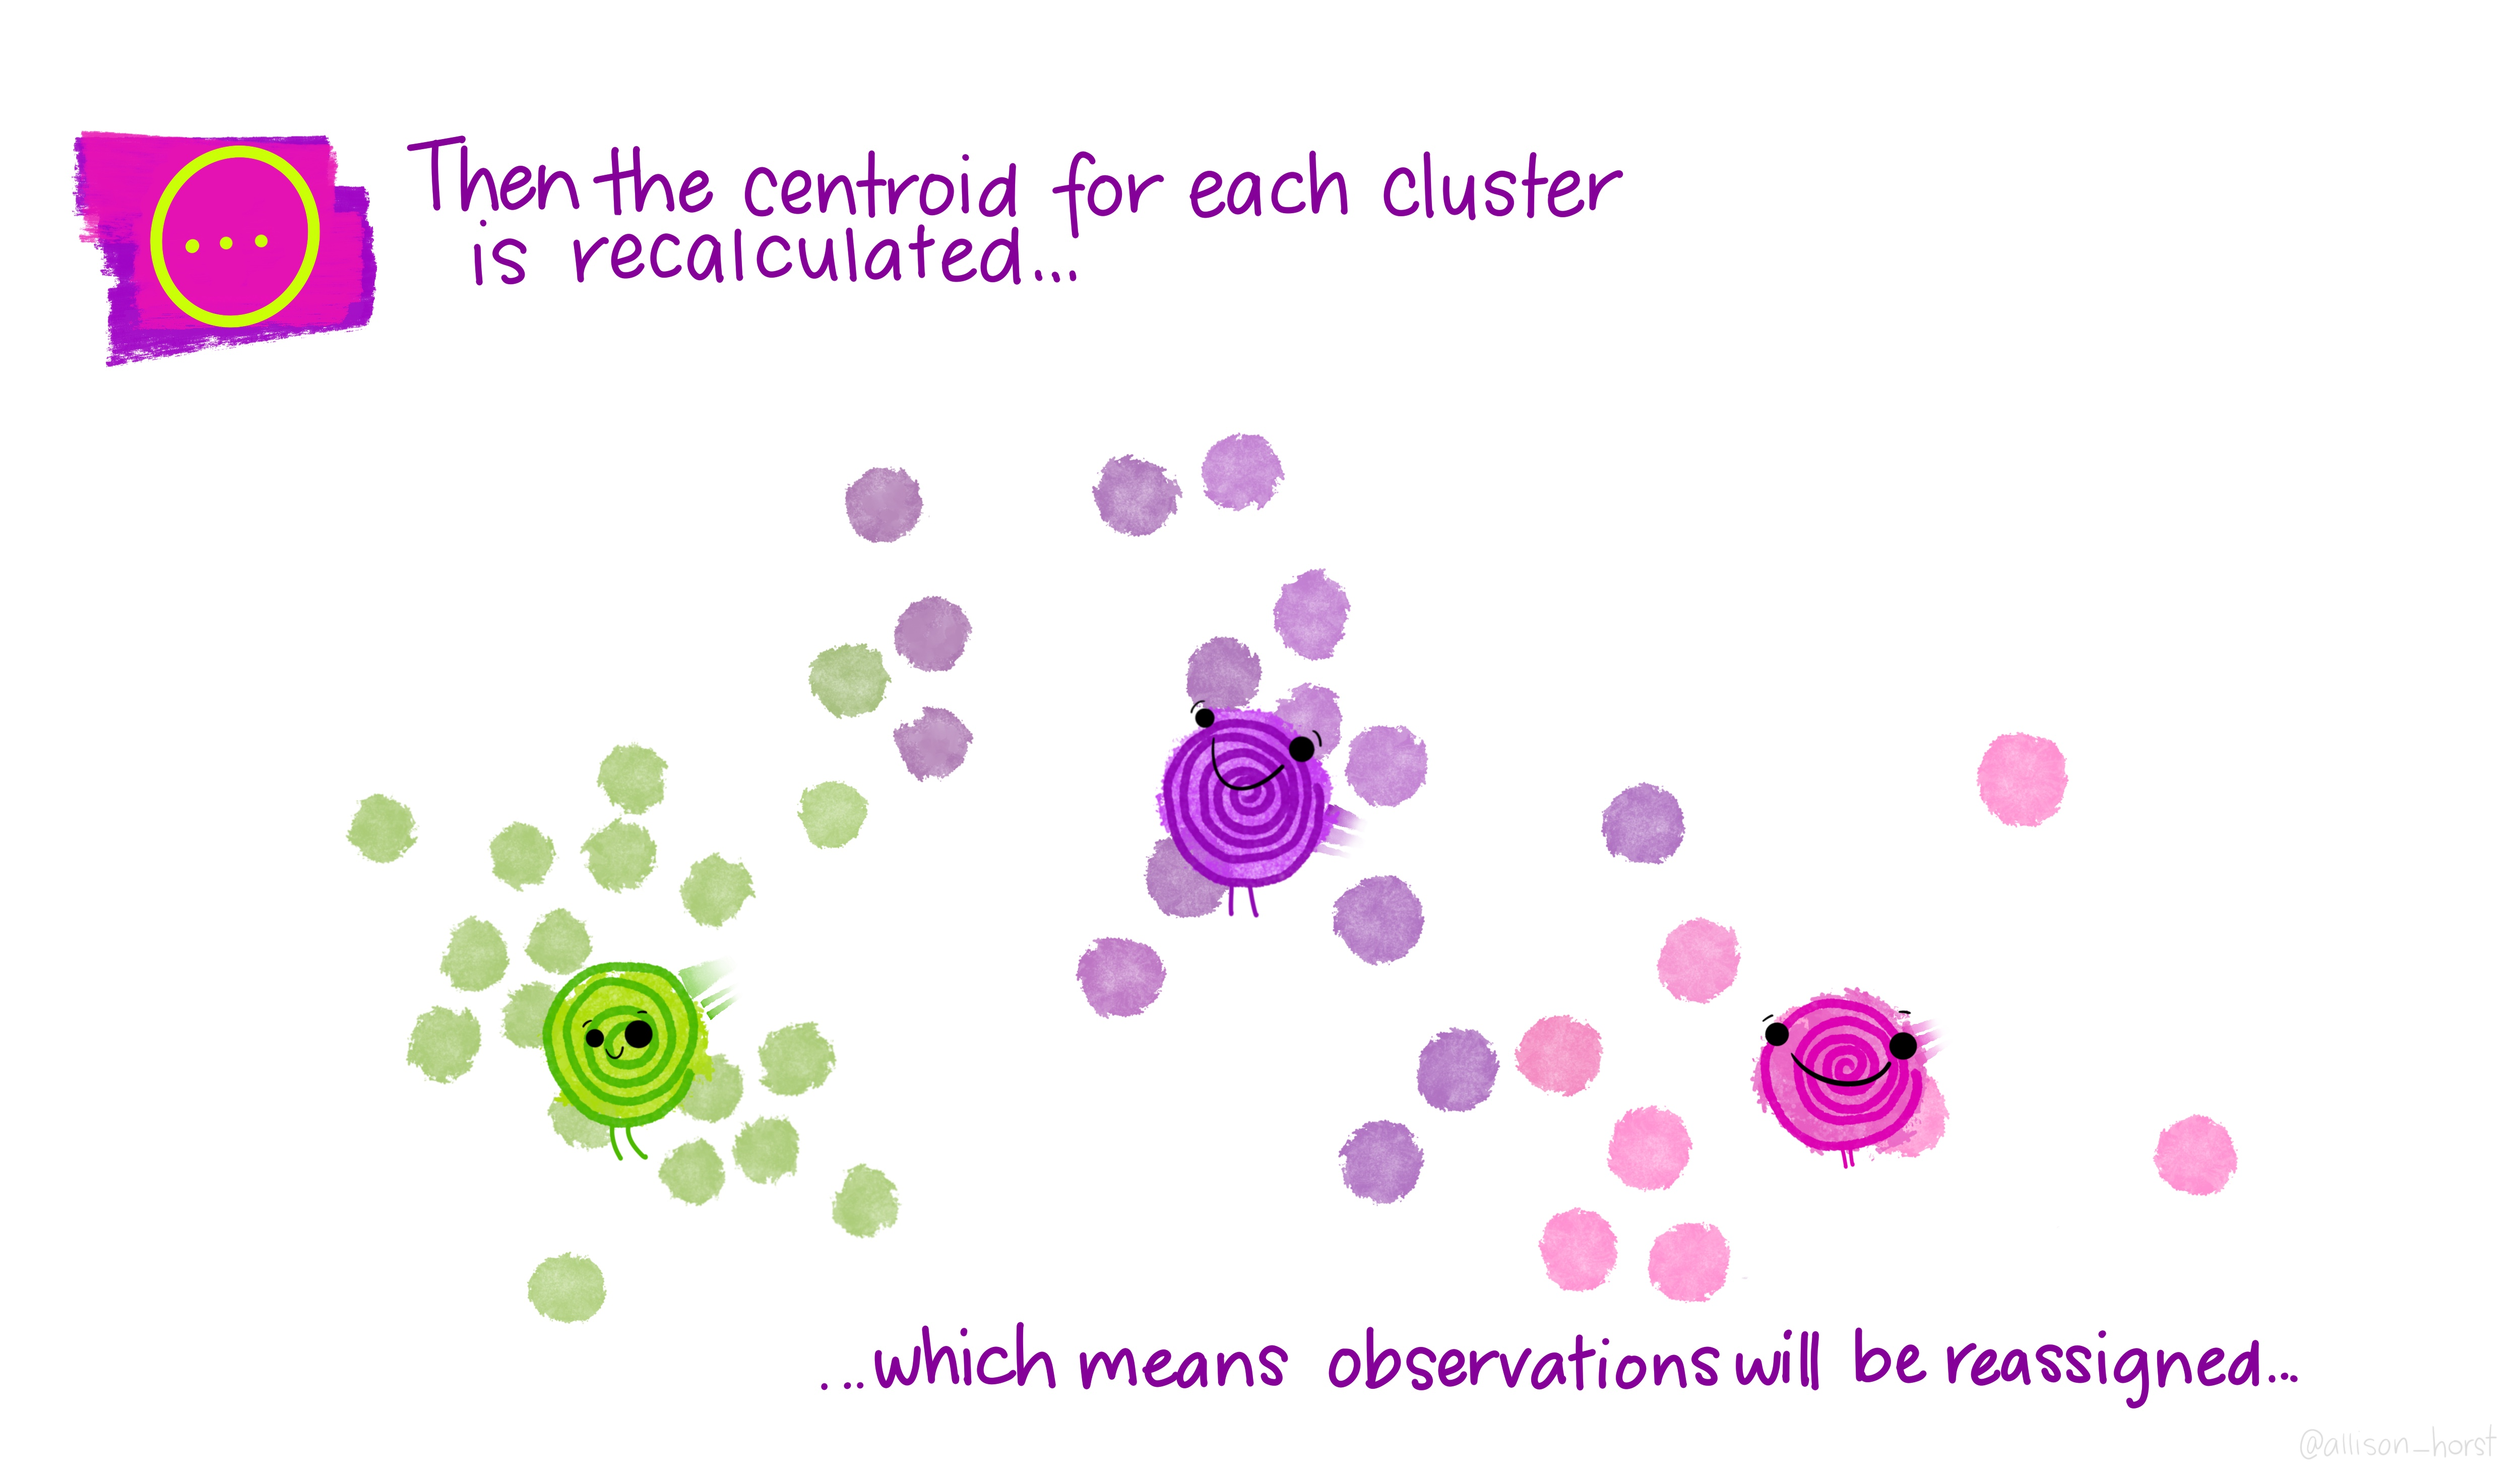
\includegraphics{figs/kmeans_10.jpg} 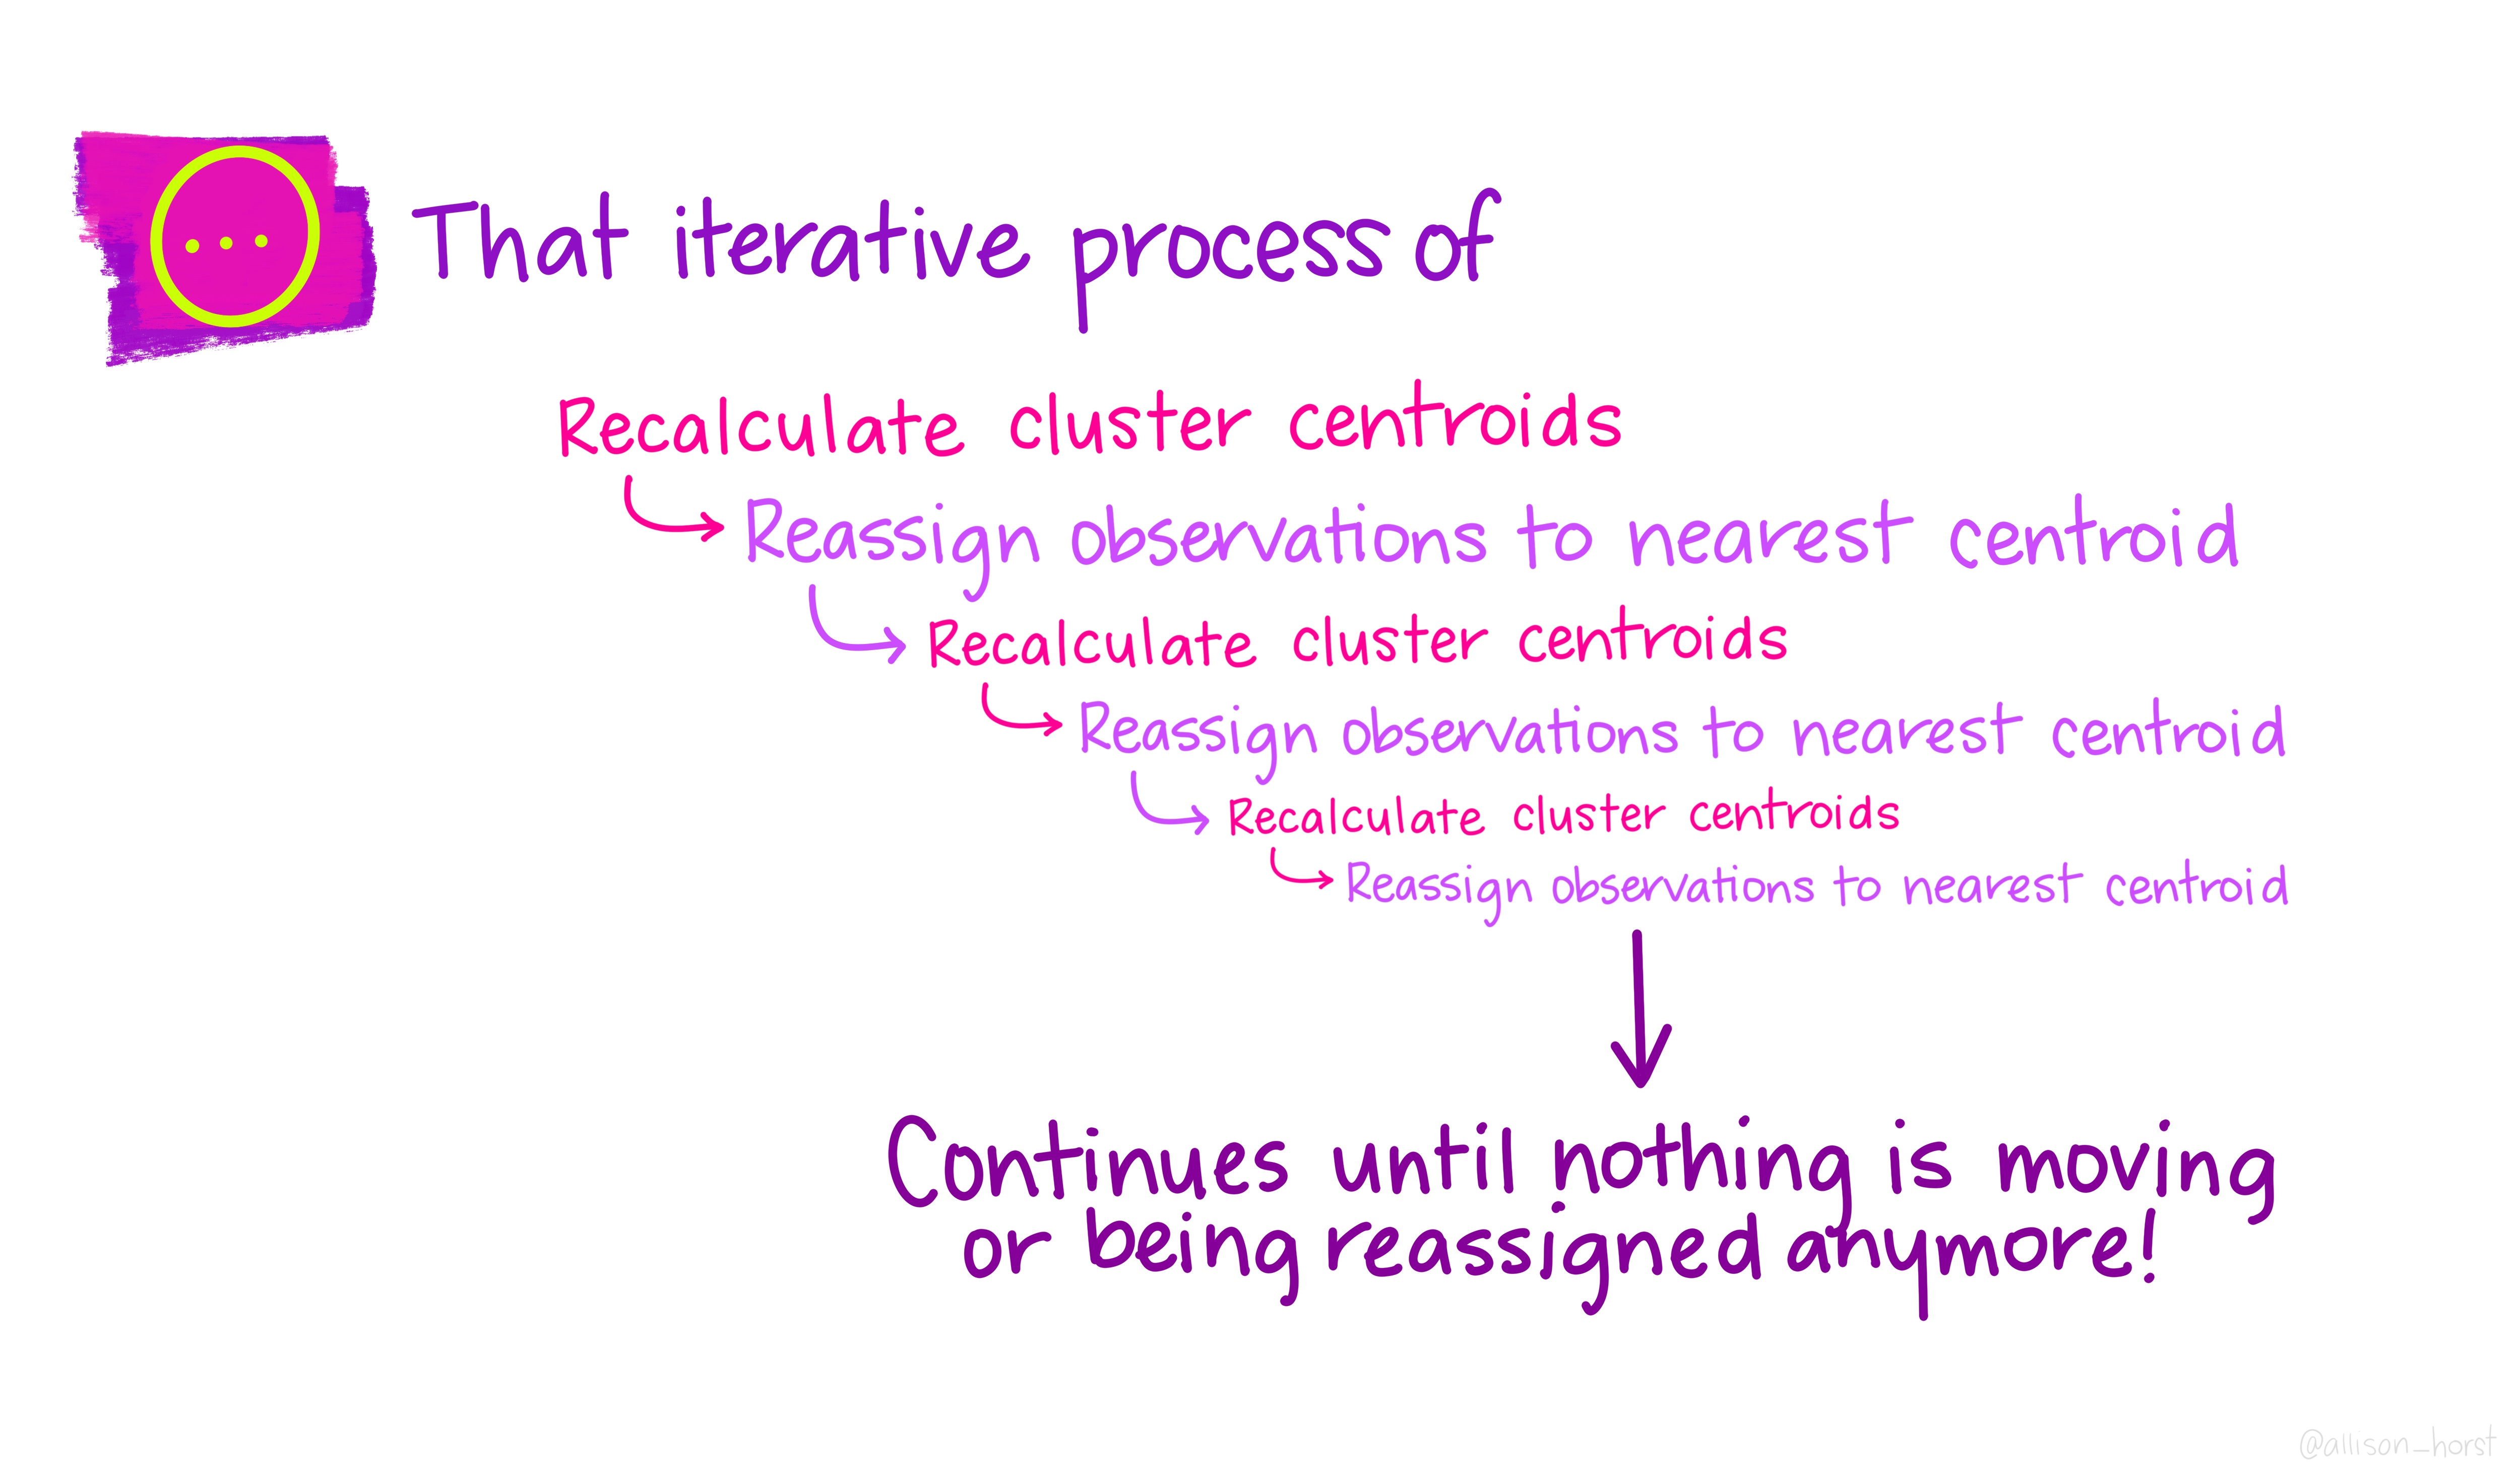
\includegraphics{figs/kmeans_11.jpg} 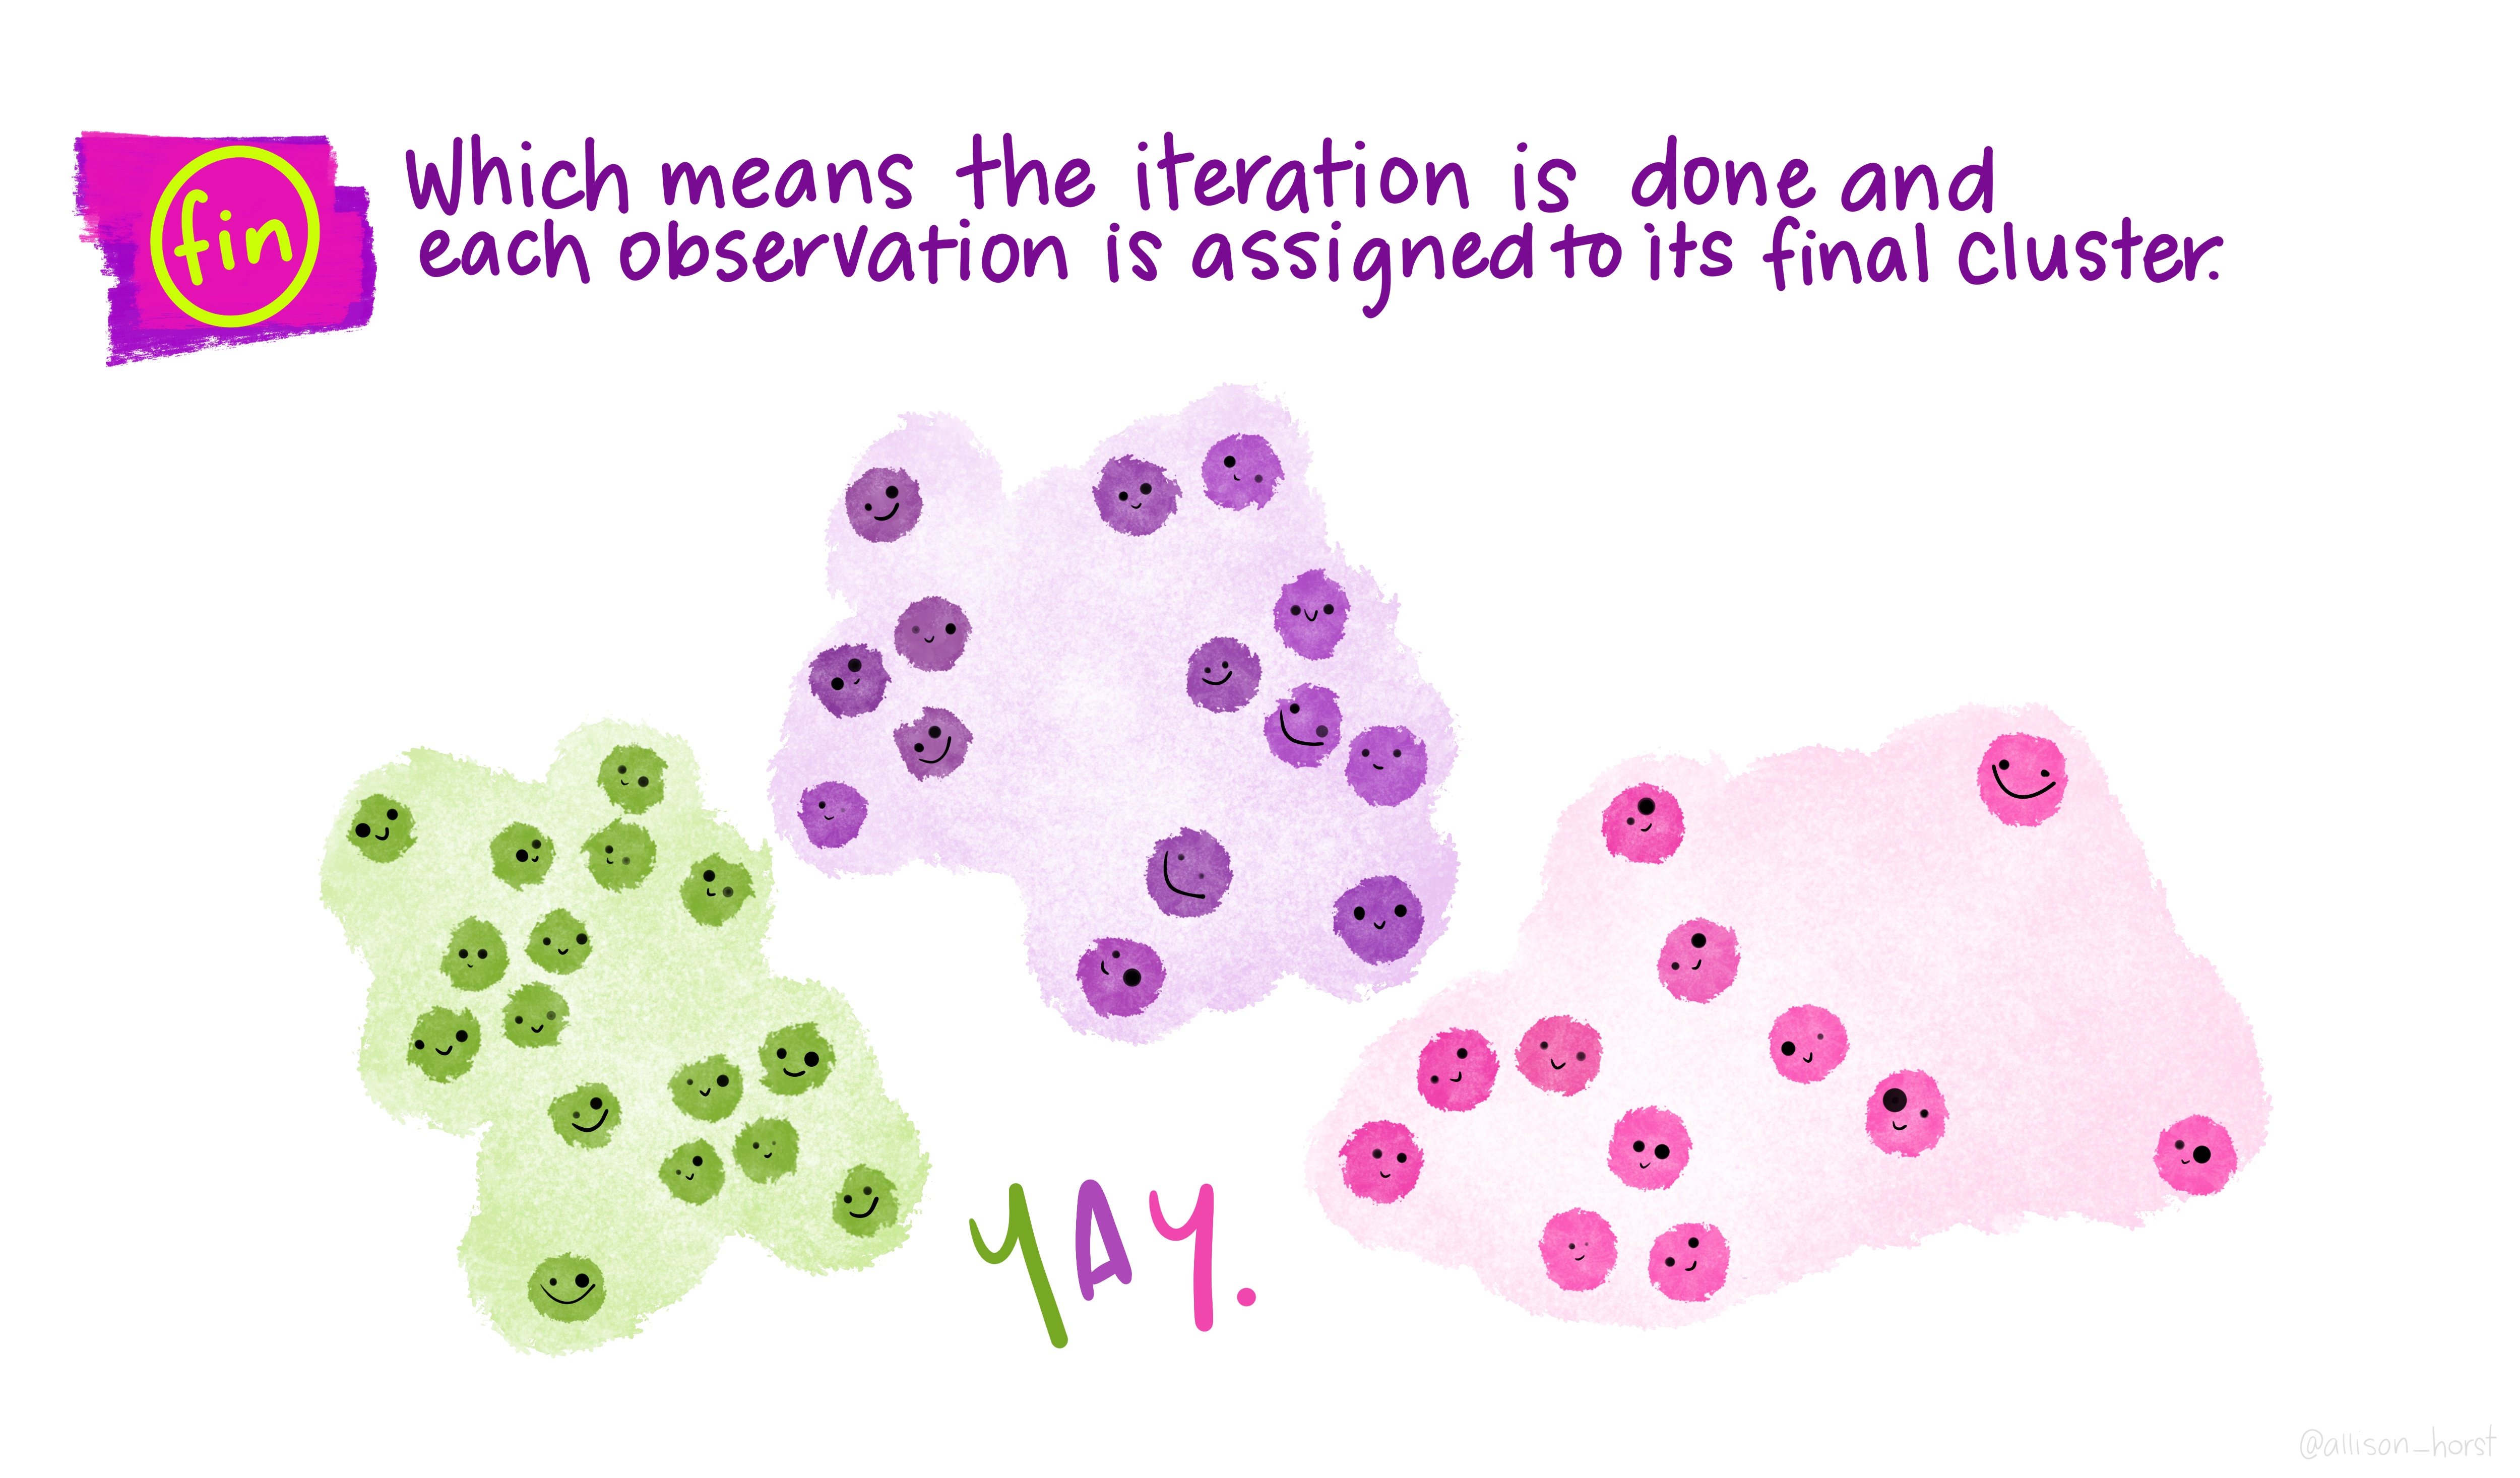
\includegraphics{figs/kmeans_12.jpg}

\hypertarget{figure-of-merit}{%
\subsection{Figure of Merit}\label{figure-of-merit}}

A limitation of this approach and of hierarchical clustering is that we may not know how many \texttt{k} clusters there are. The Figure of Merit (FOM) technique can help us work out the \texttt{k} that we need. Briefly, this works by trying a k-means clustering at 1, then 2, then 3 up to a stopping number of clusters and at the end of each clustering we check the distance variability between the centroids and the elements/cases/observations. The value of \texttt{k} that minimises the distance is the value that we want to use as most points are near to a cluster centroid.

Let's walk through the process of doing FOM and then applying a k-means clustering.

Here's a sample data set to try and cluster, we're going to cluster the rows. Note how it resembles a gene expression matrix with the gene names as the matrix row names, not in the data itself.

\begin{Shaded}
\begin{Highlighting}[]
\KeywordTok{head}\NormalTok{(gene_exprs, }\DataTypeTok{n=}\DecValTok{3}\NormalTok{)}
\end{Highlighting}
\end{Shaded}

\begin{verbatim}
##      sample1  sample2  sample3
## gn1 4.516471 3.722275 15.52375
## gn2 1.451247 3.225752 15.21140
## gn3 3.584614 3.020616 15.40538
\end{verbatim}

We'll use the \texttt{factoextra} package to do the FOM and the subsequent k-means. First the FOM using \texttt{fviz\_nbclust()}

\begin{Shaded}
\begin{Highlighting}[]
\KeywordTok{library}\NormalTok{(factoextra)}
\KeywordTok{fviz_nbclust}\NormalTok{(gene_exprs, kmeans, }\DataTypeTok{method=}\StringTok{"wss"}\NormalTok{)}
\end{Highlighting}
\end{Shaded}

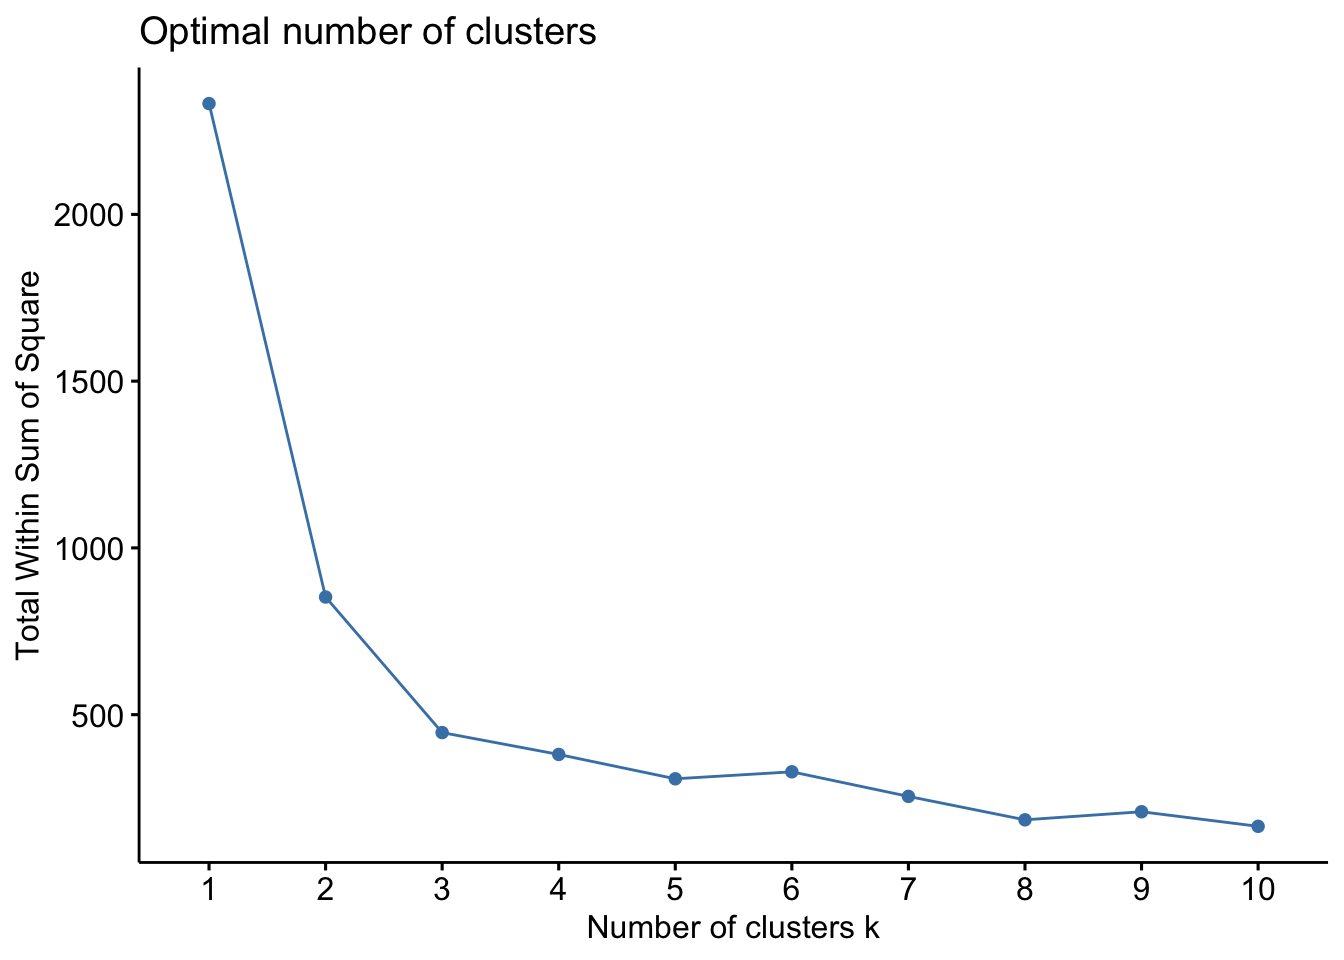
\includegraphics{machine_learning_files/figure-latex/unnamed-chunk-39-1.pdf}

The option \texttt{method} lets us specify which method we want to use to estimate the variability, here we use \texttt{wss} for within sum of squares, which is a reasonable one. The resulting plot shows that \texttt{wss} improves lots until we get to 3 clusters, at which point there is only minimal improvement. We interpret this as meaning that there are 3 clusters within our data. We can use that to make our k-means cluster. The \texttt{kmeans()} function does this easily and we can plot the result using the \texttt{fviz\_cluster()} function.

\begin{Shaded}
\begin{Highlighting}[]
\NormalTok{km_clus <-}\StringTok{ }\KeywordTok{kmeans}\NormalTok{(gene_exprs, }\DecValTok{3}\NormalTok{, }\DataTypeTok{nstart=}\DecValTok{25}\NormalTok{, }\DataTypeTok{iter.max =} \DecValTok{1000}\NormalTok{)}
\KeywordTok{fviz_cluster}\NormalTok{(km_clus, }\DataTypeTok{data=}\NormalTok{gene_exprs)}
\end{Highlighting}
\end{Shaded}

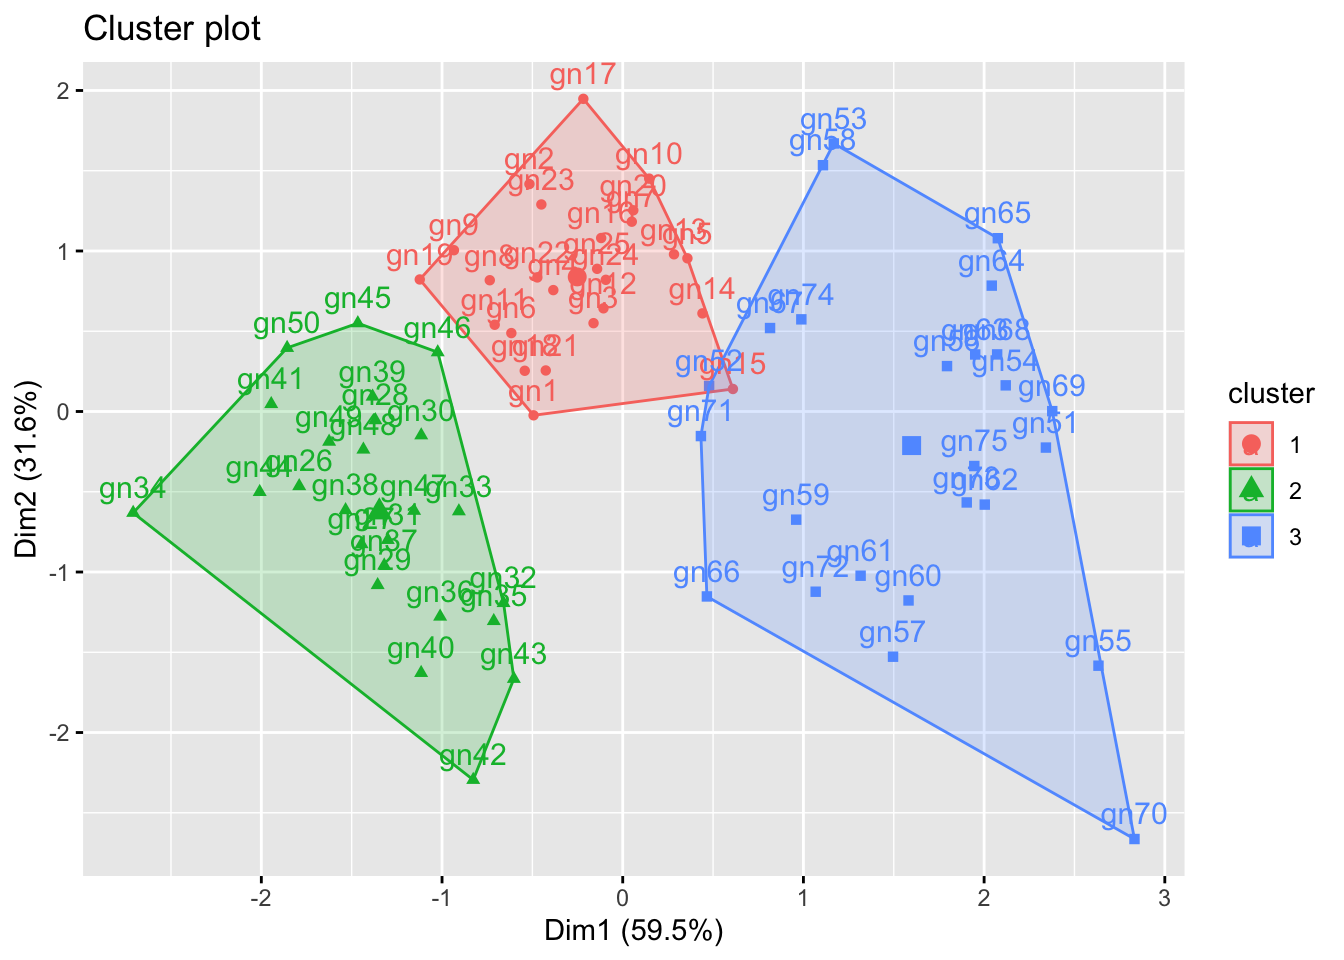
\includegraphics{machine_learning_files/figure-latex/unnamed-chunk-40-1.pdf}

The plot shows clearly the elements of the data are clustered into 3 groups. The \texttt{km\_clus} object contains information about the elements cluster membership if you wish to extract that for any reason.

\begin{roundup}
\begin{itemize}
\tightlist
\item
  Unsupervised learning algorithms group things based on distances computed between them.
\item
  Hierarchical and k-means are two common and useful methods.
\end{itemize}
\end{roundup}

\hypertarget{supervised-learning}{%
\chapter{Supervised Learning}\label{supervised-learning}}

\hypertarget{about-this-chapter-2}{%
\section{About this chapter}\label{about-this-chapter-2}}

\begin{enumerate}
\def\labelenumi{\arabic{enumi}.}
\tightlist
\item
  Questions

  \begin{itemize}
  \tightlist
  \item
    How can I find items in data that are like things I already know about?
  \end{itemize}
\item
  Objectives

  \begin{itemize}
  \tightlist
  \item
    Understand labelled data and classification
  \item
    Understand training and test data
  \item
    Understand K nearest neighbours and Random Forest
  \end{itemize}
\item
  Key Points

  \begin{itemize}
  \tightlist
  \item
    Supervised learning is classifying cases or elements based on examples that we already know
  \item
    Good training data is key
  \item
    Don't mix test and training data
  \end{itemize}
\end{enumerate}

In this chapter we'll take a look at supervised learning tools. It's called supervised learning because we have a set of data that we have already classified into one or more groups and the algorithms use that as guide and try to fit some other unknown data into the groups we've specified, so the classification is supervised in the sense that there are known examples of the groups. Again the input data is usually a data matrix of some features, like measurements or gene expression values.

\hypertarget{labelled-data}{%
\section{Labelled Data}\label{labelled-data}}

For supervised learning algorithms we need to give examples of our categories. This is called labelling the data. And in most cases we can achieve this just by extending our \(np\) features/cases data matrix by one column and add a label in there, usually as a number. For our animal matrix example that would look like this if we wanted to label our data as a cat or not.

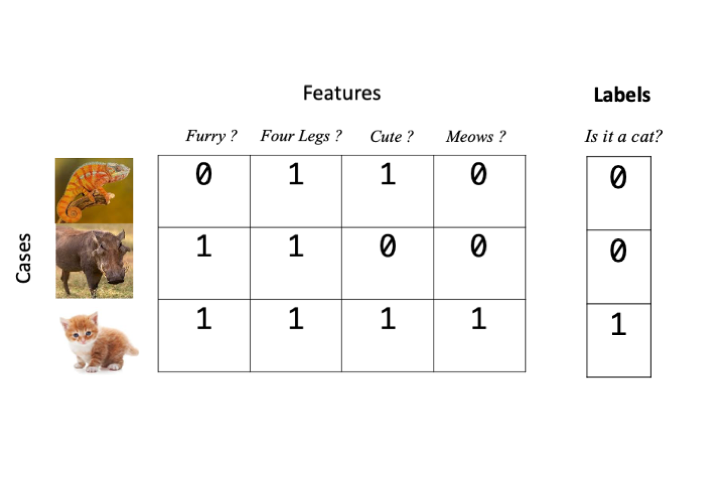
\includegraphics{figs/labels.png}

The object for the learning algorithm is then to guess labels for data that we don't know beforehand. So in our animal matrix example, that looks like this

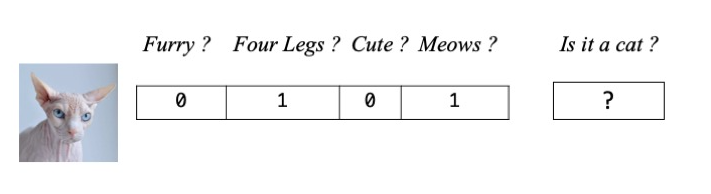
\includegraphics{figs/labels2.png}

\hypertarget{training-and-testing}{%
\section{Training and Testing}\label{training-and-testing}}

\hypertarget{the-training-phase}{%
\subsection{The Training Phase}\label{the-training-phase}}

Most supervised learning algorithms have an initial training phase. Training is a part of the procedure where the algorithm creates a model - an internal representation of the data and the associated categories or groups - that it can later use to tell which of our categories a new observation or case belong to. Each type of supervised learner has a different approach to training.

\hypertarget{the-testing-phase}{%
\subsection{The Testing Phase}\label{the-testing-phase}}

Once we have a trained model we must evaluate its accuracy. If we can't tell how accurate the model is, then we can't trust it's predictions and there is not point proceeding. We can test the model on data that \emph{we} know the labels of but that the model \emph{hasn't seen before}. The testing phase is crucial and it is imperative that we don't use the same data for testing that we used for training, doing so would be like giving a student the answers before the test. The accuracy would be artificially high as they'd already seen the right answers. Once we have a good test of the model done we can use it. Ideally, we'd want the model to give high accuracy, but that can be subjective. For some applications we might need 99\% or greater accuracy, in others just getting an answer better than random would do.

\hypertarget{measuring-accuracy}{%
\section{Measuring accuracy}\label{measuring-accuracy}}

Measuring accuracy of a model in the testing phase is less straightforward than we might first think We might assume that all we have to do is count the number of test cases that we got correct, but that is only one quarter of the story at best!. In fact, for a binary classification (a model that knows only two groups, e.g in our animal example a model that can say whether it thinks something is or isn't a cat) there are two ways to be right and two ways to be wrong and we must calculate as many of these we can in order to get a good accuracy estimate. For a model with more than two groups or for models trying to predict a quantity rather than a group the question is more complicated and we'll look at those later.

\hypertarget{two-ways-to-be-right-true-positives-and-true-negatives}{%
\subsection{Two ways to be right: True Positives and True Negatives}\label{two-ways-to-be-right-true-positives-and-true-negatives}}

The two ways to be right are to get a correct positive classification - a True Positive and a correct negative classification - a True Negative. These are easier to understand graphically. In the figure below we have a set of trained model generated answers and their true classes.

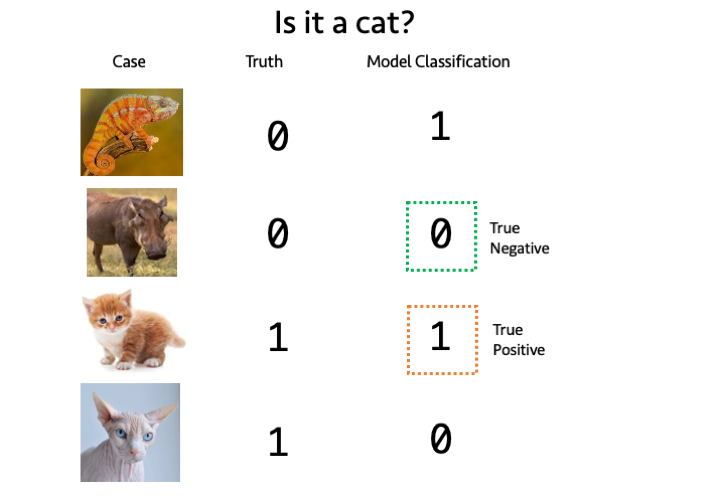
\includegraphics{figs/tptn.png}

A True Positive occurs when the model classifies a case positively (is a cat) and is correct, similarly a True Negative occurs when the model classifies a case negatively (is not a cat) and is correct.

\hypertarget{two-ways-to-be-wrong-false-postive-and-false-negatives}{%
\subsection{Two ways to be wrong: False Postive and False Negatives}\label{two-ways-to-be-wrong-false-postive-and-false-negatives}}

The two ways to be wrong are False Positive and false negative classifications False Positives and False Negatives. A False Positive occurs when the model classifies a non-cat as a cat and a False Negative occurs when the model classifies a cat as not a cat.

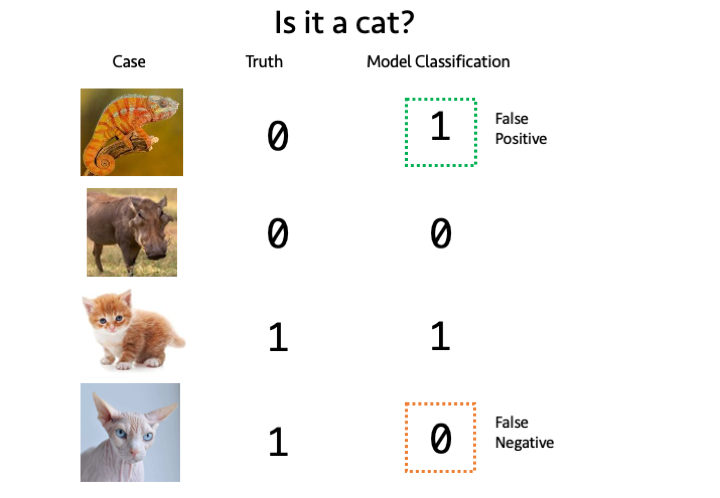
\includegraphics{figs/fpfn.png}

\hypertarget{sensitivity-and-specificity}{%
\subsection{Sensitivity and Specificity}\label{sensitivity-and-specificity}}

For a given set of test data for which we know the true labels, we run the model and get it's classifications. We can count up the True/False Positive/Negatives and calculate two quantities Sensitivity and Specificity. Sensitivity tells us roughly what proportion of True Positives we got, given the errors and Specificity tells how few wrong calls we made. The two measures are therefore complementary and are used together to get a picture of how well the model performs. A good model is high in both. The quantities are calculated as follows

\(Sensitivity = \frac{TP}{TP+FN}\)
\(Specificity = \frac{TN}{TN+FP}\)

\hypertarget{other-measures-of-accuracy}{%
\subsection{Other measures of accuracy}\label{other-measures-of-accuracy}}

There are in fact, many other measures of accuracy in use beyond sensitivity and specificity. These include things called \(F\) scores, precision and recall, FDRs and (confusingly) one actually called accuracy. It's important to know that they are all a bit different and give different measures but they all try to capture the `rightness' or `accuracy' of our classifiers. As we try out different tools we will see other measures.

\hypertarget{k-nearest-neighbours}{%
\section{\texorpdfstring{\(k\)-Nearest Neighbours}{k-Nearest Neighbours}}\label{k-nearest-neighbours}}

The \(k\)-Nearest Neighbour algorithm is a multi-class capable classification algorithm. Like the unsupervised methods this relies on distance measures between cases/elements and tries to apply a class to an unknown element by looking at the number of nearest neighbours classes. Roughly, the unknown case gets the class of the majority of the \(k\) nearest neighbours. We can see an example in the figure below

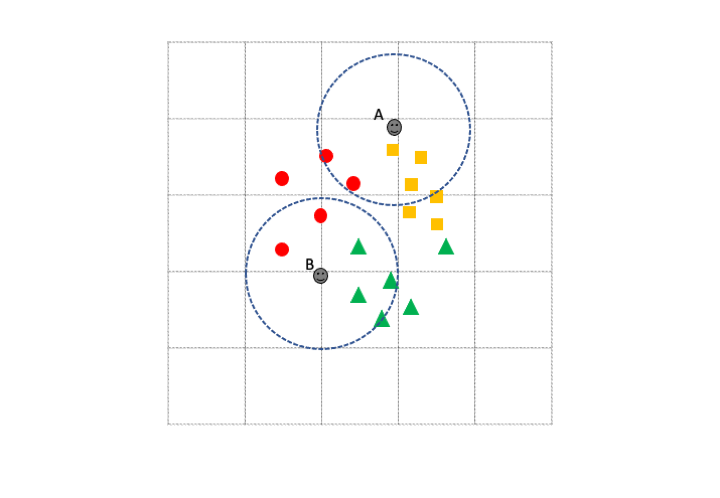
\includegraphics{figs/knn.png}

If we set \(k\) to be 5 then Unknown case A has 3 orange squares and 2 red circles in its 5 nearest neighbours, so unknown case A would be classified as an orange square. Similarly, unknown case B has more green triangles in its \(k\) nearest neighbours so it gets classified as a green triangle. Note how the known class labels are crucial in putting the unknown cases into classes. This approach only works because we have some known examples. Also note how much harder the algorithm would find the task if there were too few examples of each class. For this and many other types of supervised learning algorithm, the more training data we have, the better.

\hypertarget{training-and-evaluating-knn}{%
\subsection{\texorpdfstring{Training and evaluating \(k\)NN}{Training and evaluating kNN}}\label{training-and-evaluating-knn}}

Let's run through using the algorithm with the data below. The first phase is training and evaluation. There are 3 sets we will use, a training set of 55 points, which is labelled in a separate vector (\texttt{train\_data} and \texttt{train\_labels}), a test set of 20 points that is labelled (\texttt{test\_data} and \texttt{test\_labels}) and an unlabelled, unknown data set of 75 points that we wish to label using \(k\) Nearest Neighbours.

\begin{Shaded}
\begin{Highlighting}[]
\NormalTok{dplyr}\OperatorTok{::}\KeywordTok{glimpse}\NormalTok{(train_data)}
\end{Highlighting}
\end{Shaded}

\begin{verbatim}
## Rows: 55
## Columns: 4
## $ measure1 <dbl> 6.7, 5.4, 6.4, 5.0, 5.3, 5.4, 5.4, 5.7, 6.0, 5.1, 6.0, 5.8, 4~
## $ measure2 <dbl> 3.1, 3.4, 3.2, 3.2, 3.7, 3.9, 3.0, 4.4, 2.9, 3.8, 2.2, 2.6, 3~
## $ measure3 <dbl> 5.6, 1.7, 5.3, 1.2, 1.5, 1.7, 4.5, 1.5, 4.5, 1.9, 4.0, 4.0, 1~
## $ measure4 <dbl> 2.4, 0.2, 2.3, 0.2, 0.2, 0.4, 1.5, 0.4, 1.5, 0.4, 1.0, 1.2, 0~
\end{verbatim}

\begin{Shaded}
\begin{Highlighting}[]
\NormalTok{train_labels}
\end{Highlighting}
\end{Shaded}

\begin{verbatim}
##  [1] C A C A A A B A B A B B A A B C C A A B A B B C A A A A C C B C B A B C C B
## [39] A A B C B C C A C B A A A B B C B
## Levels: A B C
\end{verbatim}

\begin{Shaded}
\begin{Highlighting}[]
\NormalTok{dplyr}\OperatorTok{::}\KeywordTok{glimpse}\NormalTok{(test_data)}
\end{Highlighting}
\end{Shaded}

\begin{verbatim}
## Rows: 20
## Columns: 4
## $ measure1 <dbl> 5.6, 6.7, 6.3, 6.3, 5.0, 7.2, 6.2, 6.7, 4.6, 5.1, 6.0, 6.7, 7~
## $ measure2 <dbl> 3.0, 2.5, 3.3, 2.7, 2.3, 3.6, 2.2, 3.1, 3.4, 3.8, 2.2, 3.3, 3~
## $ measure3 <dbl> 4.1, 5.8, 6.0, 4.9, 3.3, 6.1, 4.5, 4.7, 1.4, 1.6, 5.0, 5.7, 6~
## $ measure4 <dbl> 1.3, 1.8, 2.5, 1.8, 1.0, 2.5, 1.5, 1.5, 0.3, 0.2, 1.5, 2.1, 2~
\end{verbatim}

\begin{Shaded}
\begin{Highlighting}[]
\NormalTok{test_labels}
\end{Highlighting}
\end{Shaded}

\begin{verbatim}
##  [1] B C C C B C B B A A C C C A A B A A B A
## Levels: A B C
\end{verbatim}

\begin{Shaded}
\begin{Highlighting}[]
\NormalTok{dplyr}\OperatorTok{::}\KeywordTok{glimpse}\NormalTok{(unknown_data)}
\end{Highlighting}
\end{Shaded}

\begin{verbatim}
## Rows: 75
## Columns: 4
## $ measure1 <dbl> 5.6, 5.0, 6.3, 6.1, 5.8, 5.5, 5.1, 5.1, 7.2, 5.0, 4.7, 7.7, 5~
## $ measure2 <dbl> 2.9, 3.6, 2.8, 2.8, 2.7, 2.6, 3.8, 3.7, 3.0, 3.0, 3.2, 2.8, 3~
## $ measure3 <dbl> 3.6, 1.4, 5.1, 4.7, 5.1, 4.4, 1.5, 1.5, 5.8, 1.6, 1.6, 6.7, 1~
## $ measure4 <dbl> 1.3, 0.2, 1.5, 1.2, 1.9, 1.2, 0.3, 0.4, 1.6, 0.2, 0.2, 2.0, 0~
\end{verbatim}

The first step is to train and test a model. As we are going to go through the process twice (one evaluating, one with unknown data), we must remember to control the random element of the algorithm. \texttt{set.seed()} with a consistent argument (\texttt{123}) puts the random number generator back to the same place each time allowing reproducibility.

The \texttt{knn()} function is in the \texttt{class} package so we load that and pass it the \texttt{train\_data} to learn from and the known \texttt{test\_data} to predict groups on. The \texttt{cl} parameter gets the vector of \texttt{train\_labels}. Finally the \(k\) nearest neighbours is passed as \texttt{k}, here \texttt{9}.

\begin{Shaded}
\begin{Highlighting}[]
\KeywordTok{set.seed}\NormalTok{(}\DecValTok{123}\NormalTok{)}
\KeywordTok{library}\NormalTok{(class)}
\NormalTok{test_set_predictions <-}\StringTok{ }\KeywordTok{knn}\NormalTok{(train_data, }\DataTypeTok{test=}\NormalTok{test_data, }\DataTypeTok{cl =}\NormalTok{ train_labels, }\DataTypeTok{k=}\DecValTok{9}\NormalTok{)}
\NormalTok{test_set_predictions}
\end{Highlighting}
\end{Shaded}

\begin{verbatim}
##  [1] B C C C B C B B A A B C C A A B A A B A
## Levels: A B C
\end{verbatim}

As we can see, the predictions are returned as vector whose elements correspond to the rows of \texttt{test\_data}. We can check the accuracy of the predictions by comparing the predictions with the known labels. The \texttt{caret} package function \texttt{confusionMatrix()} returns an object with lots of useful information.

\begin{Shaded}
\begin{Highlighting}[]
\KeywordTok{library}\NormalTok{(caret)}
\KeywordTok{confusionMatrix}\NormalTok{(test_set_predictions, test_labels)}
\end{Highlighting}
\end{Shaded}

\begin{verbatim}
## Confusion Matrix and Statistics
## 
##           Reference
## Prediction A B C
##          A 7 0 0
##          B 0 6 1
##          C 0 0 6
## 
## Overall Statistics
##                                           
##                Accuracy : 0.95            
##                  95% CI : (0.7513, 0.9987)
##     No Information Rate : 0.35            
##     P-Value [Acc > NIR] : 2.903e-08       
##                                           
##                   Kappa : 0.9251          
##                                           
##  Mcnemar's Test P-Value : NA              
## 
## Statistics by Class:
## 
##                      Class: A Class: B Class: C
## Sensitivity              1.00   1.0000   0.8571
## Specificity              1.00   0.9286   1.0000
## Pos Pred Value           1.00   0.8571   1.0000
## Neg Pred Value           1.00   1.0000   0.9286
## Prevalence               0.35   0.3000   0.3500
## Detection Rate           0.35   0.3000   0.3000
## Detection Prevalence     0.35   0.3500   0.3000
## Balanced Accuracy        1.00   0.9643   0.9286
\end{verbatim}

At the top of the output, the confusion matrix shows how `mixed' up the model got. Read it down the columns, so that for the 7 real group \texttt{A} the algorithm predicted 7 \texttt{A}, 0 \texttt{B} and 0 \texttt{C}; for the 6 real group \texttt{B} the algorithm predicted 0 \texttt{A}, 6 \texttt{B} and 0 \texttt{C} and for the 7 real group \texttt{C} the predictions were 0 \texttt{A}, 1 \texttt{B} and 6 \texttt{C}, so a \texttt{C} was misclassified as a \texttt{B}. This error rate and pattern is reflected in the overall accuracy, stated as 95 \% and the more useful per group Sensitivity and Specificity, the lower Specificity for group \texttt{B} is due to the \texttt{C} miscalled as a \texttt{B} (so a false positive \texttt{B}). The same error causes the lower Sensitivity for group \texttt{C}.

\hypertarget{using-a-trained-model}{%
\subsection{Using a trained model}\label{using-a-trained-model}}

Now that we have evaluated the model and know how accurate it is - and that it is accurate enough to be useful, we can run on our unknown data. This is virtually identical to before, replacing the \texttt{test\_data} with the \texttt{unknown\_data}. We must remember to reset the random number generator again, and we can go ahead and add the predictions straight to the data frame if we wish. We now have predicted groups for the unknown data and an estimate of the accuracy of our predictions.

\begin{Shaded}
\begin{Highlighting}[]
\KeywordTok{set.seed}\NormalTok{(}\DecValTok{123}\NormalTok{)}
\NormalTok{unknown_predictions <-}\StringTok{ }\KeywordTok{knn}\NormalTok{(train_data, }\DataTypeTok{test=}\NormalTok{unknown_data, }\DataTypeTok{cl =}\NormalTok{ train_labels, }\DataTypeTok{k=}\DecValTok{9}\NormalTok{)}
\NormalTok{unknown_data}\OperatorTok{$}\NormalTok{predicted_group <-}\StringTok{ }\NormalTok{unknown_predictions}
\NormalTok{dplyr}\OperatorTok{::}\KeywordTok{glimpse}\NormalTok{(unknown_data)}
\end{Highlighting}
\end{Shaded}

\begin{verbatim}
## Rows: 75
## Columns: 5
## $ measure1        <dbl> 5.6, 5.0, 6.3, 6.1, 5.8, 5.5, 5.1, 5.1, 7.2, 5.0, 4.7,~
## $ measure2        <dbl> 2.9, 3.6, 2.8, 2.8, 2.7, 2.6, 3.8, 3.7, 3.0, 3.0, 3.2,~
## $ measure3        <dbl> 3.6, 1.4, 5.1, 4.7, 5.1, 4.4, 1.5, 1.5, 5.8, 1.6, 1.6,~
## $ measure4        <dbl> 1.3, 0.2, 1.5, 1.2, 1.9, 1.2, 0.3, 0.4, 1.6, 0.2, 0.2,~
## $ predicted_group <fct> B, A, C, B, C, B, A, A, C, A, A, C, A, C, B, B, C, A, ~
\end{verbatim}

\hypertarget{random-forest}{%
\section{Random Forest}\label{random-forest}}

Random Forest is another supervised learning algorithm that is based on ensembles of decision trees. A decision tree is a model that resembles a question flowchart that has a `question' at each branch point and continues until enough have been `asked' to differentiate the item in hand. Here is one potential decision tree for the animal classification we've been using.

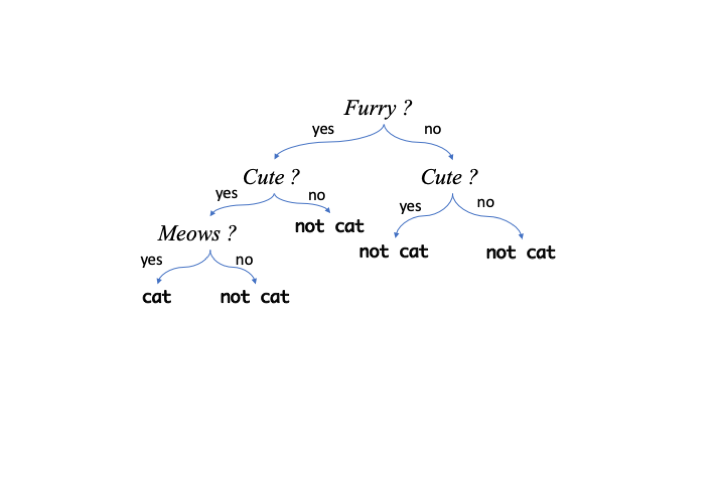
\includegraphics{figs/dt.png}

In a Random Forest classifier trees are made using the training data and the ones that are best at classifying the data are retained. There are a whole set of possible good trees so the ensemble of trees is used, hence Random Forest. The many trees make up one model that are used with unseen data.

\hypertarget{building-a-random-forest-model}{%
\subsection{Building a Random Forest Model}\label{building-a-random-forest-model}}

We use the \texttt{randomForest} package to do this, and we will use the training and test data as we did with \(k\) nearest neighbours above, for random forest, the labels are specified in the data, so we don't have a separate label vector and must now add them on to the training and test data. Let's do that first

\begin{Shaded}
\begin{Highlighting}[]
\NormalTok{train_data}\OperatorTok{$}\NormalTok{group <-}\StringTok{ }\NormalTok{train_labels}
\NormalTok{dplyr}\OperatorTok{::}\KeywordTok{glimpse}\NormalTok{(train_data)}
\end{Highlighting}
\end{Shaded}

\begin{verbatim}
## Rows: 55
## Columns: 5
## $ measure1 <dbl> 6.7, 5.4, 6.4, 5.0, 5.3, 5.4, 5.4, 5.7, 6.0, 5.1, 6.0, 5.8, 4~
## $ measure2 <dbl> 3.1, 3.4, 3.2, 3.2, 3.7, 3.9, 3.0, 4.4, 2.9, 3.8, 2.2, 2.6, 3~
## $ measure3 <dbl> 5.6, 1.7, 5.3, 1.2, 1.5, 1.7, 4.5, 1.5, 4.5, 1.9, 4.0, 4.0, 1~
## $ measure4 <dbl> 2.4, 0.2, 2.3, 0.2, 0.2, 0.4, 1.5, 0.4, 1.5, 0.4, 1.0, 1.2, 0~
## $ group    <fct> C, A, C, A, A, A, B, A, B, A, B, B, A, A, B, C, C, A, A, B, A~
\end{verbatim}

We can now build the model with the \texttt{randomForest()} function. The setup uses R's formula based syntax, so is very similar to that we used for linear models. The \texttt{group} is to be predicted based on \texttt{.} which means all other columns in the data \texttt{train\_data}. The \texttt{model} variable holds the trained model

\begin{Shaded}
\begin{Highlighting}[]
\KeywordTok{library}\NormalTok{(randomForest)}
\NormalTok{model <-}\StringTok{ }\KeywordTok{randomForest}\NormalTok{(group }\OperatorTok{~}\StringTok{ }\NormalTok{., }\DataTypeTok{data =}\NormalTok{ train_data, }\DataTypeTok{mtry=}\DecValTok{2}\NormalTok{)}
\end{Highlighting}
\end{Shaded}

\hypertarget{testing-a-random-forest-model}{%
\subsection{Testing a Random Forest model}\label{testing-a-random-forest-model}}

With the model built we can use the generic \texttt{predict()} function to get the model to predict groups for the unlabelled \texttt{test\_data} then compare it to the real groups with \texttt{confusionMatrix()}. Setting the value of \texttt{type} to \texttt{class} tells the \texttt{predict()} we want group classifications

\begin{Shaded}
\begin{Highlighting}[]
\NormalTok{test_set_predictions <-}\StringTok{ }\KeywordTok{predict}\NormalTok{(model, test_data, }\DataTypeTok{type=}\StringTok{"class"}\NormalTok{)}
\KeywordTok{confusionMatrix}\NormalTok{(test_set_predictions, test_labels)}
\end{Highlighting}
\end{Shaded}

\begin{verbatim}
## Confusion Matrix and Statistics
## 
##           Reference
## Prediction A B C
##          A 7 0 0
##          B 0 6 1
##          C 0 0 6
## 
## Overall Statistics
##                                           
##                Accuracy : 0.95            
##                  95% CI : (0.7513, 0.9987)
##     No Information Rate : 0.35            
##     P-Value [Acc > NIR] : 2.903e-08       
##                                           
##                   Kappa : 0.9251          
##                                           
##  Mcnemar's Test P-Value : NA              
## 
## Statistics by Class:
## 
##                      Class: A Class: B Class: C
## Sensitivity              1.00   1.0000   0.8571
## Specificity              1.00   0.9286   1.0000
## Pos Pred Value           1.00   0.8571   1.0000
## Neg Pred Value           1.00   1.0000   0.9286
## Prevalence               0.35   0.3000   0.3500
## Detection Rate           0.35   0.3000   0.3000
## Detection Prevalence     0.35   0.3500   0.3000
## Balanced Accuracy        1.00   0.9643   0.9286
\end{verbatim}

The model is again, convincing and highly accurate so we can repeat use \texttt{predict()} with \texttt{model} to get predictions for \texttt{unknown\_data}, and again add it to the data

\begin{Shaded}
\begin{Highlighting}[]
\NormalTok{unknown_predictions <-}\StringTok{ }\KeywordTok{predict}\NormalTok{(model, unknown_data, }\DataTypeTok{type=}\StringTok{"class"}\NormalTok{)}
\NormalTok{unknown_data}\OperatorTok{$}\NormalTok{predicted_group <-}\StringTok{ }\NormalTok{unknown_predictions}
\NormalTok{dplyr}\OperatorTok{::}\KeywordTok{glimpse}\NormalTok{(unknown_data)}
\end{Highlighting}
\end{Shaded}

\begin{verbatim}
## Rows: 75
## Columns: 5
## $ measure1        <dbl> 5.6, 5.0, 6.3, 6.1, 5.8, 5.5, 5.1, 5.1, 7.2, 5.0, 4.7,~
## $ measure2        <dbl> 2.9, 3.6, 2.8, 2.8, 2.7, 2.6, 3.8, 3.7, 3.0, 3.0, 3.2,~
## $ measure3        <dbl> 3.6, 1.4, 5.1, 4.7, 5.1, 4.4, 1.5, 1.5, 5.8, 1.6, 1.6,~
## $ measure4        <dbl> 1.3, 0.2, 1.5, 1.2, 1.9, 1.2, 0.3, 0.4, 1.6, 0.2, 0.2,~
## $ predicted_group <fct> B, A, C, B, C, B, A, A, C, A, A, C, A, C, B, B, C, A, ~
\end{verbatim}

\hypertarget{random-forest-with-categorical-predictors}{%
\subsection{Random Forest with categorical predictors}\label{random-forest-with-categorical-predictors}}

In our \(k\)NN example and the previous Random Forest predictor, the input data features were solely numeric. Random Forest can handle a mixture of numeric and character or categorical based features allowing us to make classifications on more than numbers. The process is similar, so let's get some appropriate data and do that

\begin{Shaded}
\begin{Highlighting}[]
\NormalTok{dplyr}\OperatorTok{::}\KeywordTok{glimpse}\NormalTok{(train_data_mixed)}
\end{Highlighting}
\end{Shaded}

\begin{verbatim}
## Rows: 55
## Columns: 6
## $ measure1 <dbl> 6.7, 5.4, 6.4, 5.0, 5.3, 5.4, 5.4, 5.7, 6.0, 5.1, 6.0, 5.8, 4~
## $ measure2 <dbl> 3.1, 3.4, 3.2, 3.2, 3.7, 3.9, 3.0, 4.4, 2.9, 3.8, 2.2, 2.6, 3~
## $ measure3 <dbl> 5.6, 1.7, 5.3, 1.2, 1.5, 1.7, 4.5, 1.5, 4.5, 1.9, 4.0, 4.0, 1~
## $ measure4 <dbl> 2.4, 0.2, 2.3, 0.2, 0.2, 0.4, 1.5, 0.4, 1.5, 0.4, 1.0, 1.2, 0~
## $ group    <fct> C, A, C, A, A, A, B, A, B, A, B, B, A, A, B, C, C, A, A, B, A~
## $ colour   <fct> White, Green, White, Green, Green, Green, Blue, Green, Blue, ~
\end{verbatim}

\begin{Shaded}
\begin{Highlighting}[]
\NormalTok{dplyr}\OperatorTok{::}\KeywordTok{glimpse}\NormalTok{(test_data_mixed)}
\end{Highlighting}
\end{Shaded}

\begin{verbatim}
## Rows: 20
## Columns: 6
## $ measure1 <dbl> 5.6, 6.7, 6.3, 6.3, 5.0, 7.2, 6.2, 6.7, 4.6, 5.1, 6.0, 6.7, 7~
## $ measure2 <dbl> 3.0, 2.5, 3.3, 2.7, 2.3, 3.6, 2.2, 3.1, 3.4, 3.8, 2.2, 3.3, 3~
## $ measure3 <dbl> 4.1, 5.8, 6.0, 4.9, 3.3, 6.1, 4.5, 4.7, 1.4, 1.6, 5.0, 5.7, 6~
## $ measure4 <dbl> 1.3, 1.8, 2.5, 1.8, 1.0, 2.5, 1.5, 1.5, 0.3, 0.2, 1.5, 2.1, 2~
## $ group    <fct> B, C, C, C, B, C, B, B, A, A, C, C, C, A, A, B, A, A, B, A
## $ colour   <fct> Blue, White, White, White, Blue, White, Blue, Blue, Green, Gr~
\end{verbatim}

\begin{Shaded}
\begin{Highlighting}[]
\NormalTok{dplyr}\OperatorTok{::}\KeywordTok{glimpse}\NormalTok{(unknown_data_mixed)}
\end{Highlighting}
\end{Shaded}

\begin{verbatim}
## Rows: 75
## Columns: 6
## $ measure1 <dbl> 5.6, 5.0, 6.3, 6.1, 5.8, 5.5, 5.1, 5.1, 7.2, 5.0, 4.7, 7.7, 5~
## $ measure2 <dbl> 2.9, 3.6, 2.8, 2.8, 2.7, 2.6, 3.8, 3.7, 3.0, 3.0, 3.2, 2.8, 3~
## $ measure3 <dbl> 3.6, 1.4, 5.1, 4.7, 5.1, 4.4, 1.5, 1.5, 5.8, 1.6, 1.6, 6.7, 1~
## $ measure4 <dbl> 1.3, 0.2, 1.5, 1.2, 1.9, 1.2, 0.3, 0.4, 1.6, 0.2, 0.2, 2.0, 0~
## $ colour   <fct> Blue, Green, White, Blue, White, Blue, Green, Green, White, G~
## $ group    <fct> B, A, C, B, C, B, A, A, C, A, A, C, A, C, B, B, C, A, C, B, A~
\end{verbatim}

We can see that there is a new categorical feature called \texttt{colour} in our train and test data, but not in our unknown data, so let's try to predict the colour this time.

\begin{Shaded}
\begin{Highlighting}[]
\NormalTok{model2 <-}\StringTok{ }\KeywordTok{randomForest}\NormalTok{(colour }\OperatorTok{~}\StringTok{ }\NormalTok{., }\DataTypeTok{data =}\NormalTok{ train_data_mixed, }\DataTypeTok{mtry=}\DecValTok{2}\NormalTok{)}

\NormalTok{test_set_mixed_predictions <-}\StringTok{ }\KeywordTok{predict}\NormalTok{(model2, test_data_mixed, }\DataTypeTok{type=}\StringTok{"class"}\NormalTok{)}
\KeywordTok{confusionMatrix}\NormalTok{(test_set_mixed_predictions, test_labels_mixed)}
\end{Highlighting}
\end{Shaded}

\begin{verbatim}
## Confusion Matrix and Statistics
## 
##           Reference
## Prediction Blue Green White
##      Blue     6     0     0
##      Green    0     7     0
##      White    0     0     7
## 
## Overall Statistics
##                                      
##                Accuracy : 1          
##                  95% CI : (0.8316, 1)
##     No Information Rate : 0.35       
##     P-Value [Acc > NIR] : 7.61e-10   
##                                      
##                   Kappa : 1          
##                                      
##  Mcnemar's Test P-Value : NA         
## 
## Statistics by Class:
## 
##                      Class: Blue Class: Green Class: White
## Sensitivity                  1.0         1.00         1.00
## Specificity                  1.0         1.00         1.00
## Pos Pred Value               1.0         1.00         1.00
## Neg Pred Value               1.0         1.00         1.00
## Prevalence                   0.3         0.35         0.35
## Detection Rate               0.3         0.35         0.35
## Detection Prevalence         0.3         0.35         0.35
## Balanced Accuracy            1.0         1.00         1.00
\end{verbatim}

So we have created a model that is capable of perfectly predicting the value of the categoric value colour from a mixture of numeric and categoric features. Why is the model so accurate? It's a bit of a fix! This sample data has a direct mapping between the \texttt{group} and the \texttt{colour}: \texttt{A} is always \texttt{Green}, \texttt{B} is always \texttt{Blue} and \texttt{C} is always \texttt{White} so it is easy to predict colour if you have \texttt{group}. The data aren't typical in this sense but it does highlight the procedure.

\hypertarget{random-forest-regression}{%
\subsection{Random Forest Regression}\label{random-forest-regression}}

It is also possible to perform prediction of numeric values and not just classes with Random Forest. We simply set up the model with a numeric value as the predicted value in the formula as follows

\begin{Shaded}
\begin{Highlighting}[]
\NormalTok{model3 <-}\StringTok{ }\KeywordTok{randomForest}\NormalTok{(measure1 }\OperatorTok{~}\StringTok{ }\NormalTok{., }\DataTypeTok{data =}\NormalTok{ train_data_mixed, }\DataTypeTok{mtry=}\DecValTok{2}\NormalTok{)}
\end{Highlighting}
\end{Shaded}

Now when we use \texttt{predict()} and omit the \texttt{type} argument, we get a set of numbers, not classes back

\begin{Shaded}
\begin{Highlighting}[]
\NormalTok{test_set_mixed_predictions_numeric <-}\StringTok{ }\KeywordTok{predict}\NormalTok{(model3, test_data_mixed)}
\NormalTok{test_set_mixed_predictions_numeric}
\end{Highlighting}
\end{Shaded}

\begin{verbatim}
##       89      109      101      124       94      110       69       87 
## 5.966036 6.237482 6.900857 6.007691 5.517170 6.887034 5.695914 6.222375 
##        7       47      120      125      118        1       15       96 
## 5.039731 5.181784 5.838623 6.722102 6.891138 5.088806 5.109832 5.982576 
##       24       38       88       48 
## 5.263310 5.012233 5.735793 4.833798
\end{verbatim}

\hypertarget{evaluating-numeric-predictions}{%
\subsubsection{Evaluating numeric predictions}\label{evaluating-numeric-predictions}}

Previously we've evaluated predictions from our models for classes, counting True Positives etc, but we can't do that here because we have no classes. Instead we can calculate how far away from the real value the predictions are on average. That's a simple sum to do in R

\begin{Shaded}
\begin{Highlighting}[]
\KeywordTok{mean}\NormalTok{( (test_data_mixed}\OperatorTok{$}\NormalTok{measure1 }\OperatorTok{-}\StringTok{ }\NormalTok{test_set_mixed_predictions_numeric) }\OperatorTok{^}\StringTok{ }\DecValTok{2}\NormalTok{)}
\end{Highlighting}
\end{Shaded}

\begin{verbatim}
## [1] 0.1745713
\end{verbatim}

The quantity is called the Mean Squared Error or MSE. The lower the better, though the actual size is dependent on context. The context here is the descriptive statistics of the known values for the test data, which we can get with \texttt{summary()}

\begin{Shaded}
\begin{Highlighting}[]
\KeywordTok{summary}\NormalTok{(test_data_mixed}\OperatorTok{$}\NormalTok{measure1)}
\end{Highlighting}
\end{Shaded}

\begin{verbatim}
##    Min. 1st Qu.  Median    Mean 3rd Qu.    Max. 
##    4.60    5.10    5.90    5.88    6.40    7.70
\end{verbatim}

These values range between 4.6 and 7.7, with 50\% of them lying between 5.1 and 6.4. With that in mind it seems like an MSE of 0.17 is a pretty good result and we can conclude to predict accurately the values of \texttt{measure1} from our Random Forest Regression model.

\begin{roundup}
\begin{itemize}
\tightlist
\item
  Supervised Learning uses labelled data to make predictions on unseen data
\item
  Random Forest can predict classes and numeric values (perform regression)
\item
  It is imperative to evaluate the predictive model on a set of known cases
\end{itemize}
\end{roundup}

\hypertarget{deep-learning}{%
\chapter{Deep Learning}\label{deep-learning}}

\begin{enumerate}
\def\labelenumi{\arabic{enumi}.}
\tightlist
\item
  Questions

  \begin{itemize}
  \tightlist
  \item
    What is Deep Learning?
  \item
    How is Deep Learning distinct from classical Machine Learning?
  \end{itemize}
\item
  Objectives

  \begin{itemize}
  \tightlist
  \item
    Discuss how cryptic patterns can find their own important features in arbitrary data sets
  \item
    Study the outline of training a Neural Network
  \item
    Build and test a simple Neural Network
  \end{itemize}
\item
  Key Points

  \begin{itemize}
  \tightlist
  \item
    Deep Learners find important features and patterns in the data automatically
  \item
    Neural Networks use optimised weights to learn classifications
  \item
    Power comes at the expense of interpretability
  \end{itemize}
\end{enumerate}

\hypertarget{about-this-chapter-3}{%
\section{About this chapter}\label{about-this-chapter-3}}

In this chapter we'll look at the latest advance in Machine Learning, a special set of extremely powerful techniques called Deep Learning. Deep learning methods are the ones that have been used in headline grabbing Artificial Intelligence toold from large scale facial recognition, data mining to influence voters on social media, voice recognition like Siri and Alexa, Netflix's suggestion algorithm, Google's advertising algorithm, and in science things like AlphaFold - the protein folding prediction tool and medical image analysis.

These tools and algorithms are a wide family of their own and have properties distinct from the machine learning techniques we've looked at so far, principally these types are able to select the most important features themselves and work out what is the most reliable data. They are also much more complicated in practice and much more dense so they become a black box and we are less able to interpret how they are making the decisions they make. This is the trade off we make when using Deep Learning.

\hypertarget{feature-selection-in-deep-learning}{%
\section{Feature Selection in Deep Learning}\label{feature-selection-in-deep-learning}}

In the previous tools we've looked at we used a \(np\) feature matrix, with \(p\) features - a column of data for each thing we measured. Feature selection is really important and can make or break the usefulness of a machine learning tool. If the features we select can't differentiate between the classes, then the machine learning tool will never be able to make good predictions. Consider what it would be like if we tried to work out a person's hair colour from their height! Height is an easy thing to measure but does it ever predict a person's hair?

So we must pick our features carefully if we're to make use of ML generally, but with Deep Learning the algorithms themselves work out which are the most useful features and also patterns within the features and preferentially use them. This leads to a bit of a kitchen sink approach, we can take all the features we like, pump them into a Deep Learning algorithm and let it decide the best way to use them. A practical upside of this then is that our \(np\) feature matrix can become very complicated and we can start to squeeze pretty much anything into the training data. We simply have to be able to encode it as numbers somehow.

\hypertarget{cryptic-patterns-in-deep-learning}{%
\section{Cryptic patterns in Deep Learning}\label{cryptic-patterns-in-deep-learning}}

The ability to automatically select features or patterns to use means that the algorithms can find and use patterns that we don't specify explicitly and in fact don't even know about. To understand this, let's work through a protein sequence based example. Our first issue with biological sequences is the question of how to encode it as numbers. One common way of taking a categoric thing and making it numeric is to use `One Hot Encoding'. Which looks like this:

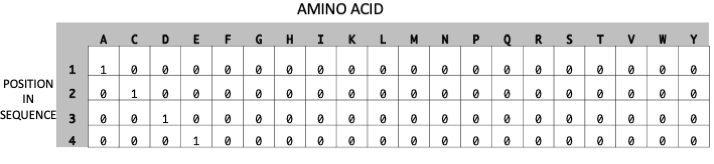
\includegraphics{figs/onehot.png}

This encoding represents the protein sequence `ACDE', the columns represent the alphabet of amino acids (in alphabetic order), the rows represent the position of sequence. We add a \texttt{1} at the intersection of the position and amino acid to show the amino acid at each position. Each row therefore has only one row.

Once we have an encoding, patterns will start to appear that the algorithms can use. Consider a protein motif, like RHLR - that would look like this in our one hot encoding.

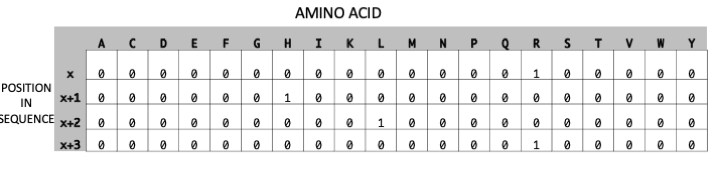
\includegraphics{figs/rhlr.png}

Now wherever the pattern crops up the algorithm will see it. The pattern can become associated with a particular class and used as part of the signal for classification. We didn't have to say `protein has RHLR', if it's an important pattern and associated with a class or group then the algorithm will use it.

\hypertarget{implications-of-cryptic-patterns}{%
\subsection{Implications of Cryptic Patterns}\label{implications-of-cryptic-patterns}}

Being able to select its own features and patterns means that the Deep Learning methods get a special sort of sensitivity. Considering our protein example again, then lots of properties of the proteins that are reliant on sequence at some level will be detectable and useable in some way by the Deep Learner. Things like physico-chemical sequence properties such as hydrophobicity are reliant on the actual amino acids to exist so they can be captured and used.

An important thing to note is that the patterns have only to be associated, not \emph{over-represented}, on the whole. The Deep Learners might find a pattern that occurs only a few times in millions of example data, but if it is associated pretty uniquely with just one class or group then it can be used. This stands in contrast to typical methods of pattern finding in bioinformatics, which use majority or statistical over-representation. The patterns often have weight with other patterns and these associations increase the patterns power too.

The ability to find cryptic patterns and make associations is reliant on having a great deal of training data. Deep Learning methods do require lots more data than the ML methods we've already looked at and this can be a drawback in practice.

Deep Learning models internal representations become very large and hard to interpret, so that actually understanding what they're using to classify upon can become impossible. This is a significant trade off for the high power that we can get

\hypertarget{neural-networks}{%
\section{Neural Networks}\label{neural-networks}}

The core of most Deep Learning models and model types is the neural network, let's run through how that works to gain some insight into how it gets its power.

\hypertarget{the-perceptron}{%
\subsection{The Perceptron}\label{the-perceptron}}

Neural networks are made up of units called Perceptrons, these are mathematical structures inspired by biological neurons. They take multiple inputs, integrate them in some way and produce an output. One that worked on our animal matrix might look like this

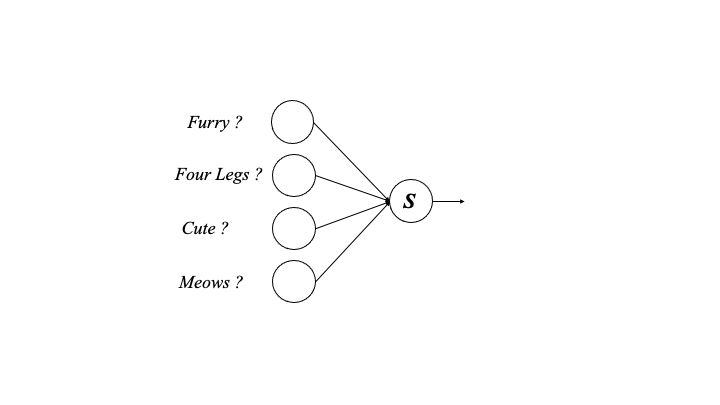
\includegraphics{figs/percepwts/Slide1.png}

\hypertarget{the-network}{%
\subsection{The Network}\label{the-network}}

Combining lots of perceptrons results in a neural network and at a basic level might work with our animal data like this,

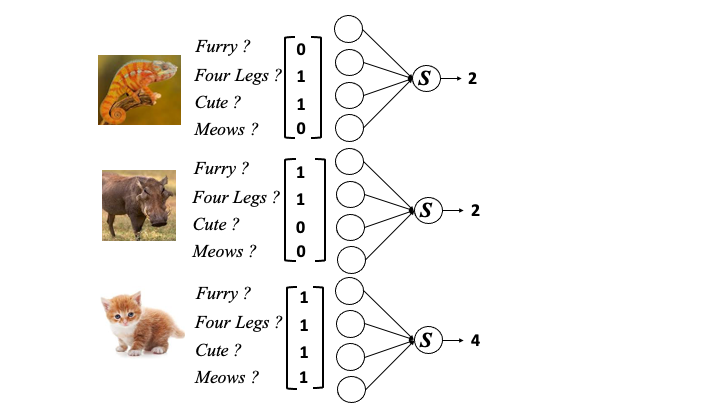
\includegraphics{figs/percepwts/Slide2.png}

Making sense of all the integrations from the neural network, that is the calling of a class (in this case \texttt{is\_a\_cat}) is done by a decision function, here that may look like this

\begin{verbatim}
if S > 2,
    cat = 1
else 
    cat = 0
\end{verbatim}

Applied to the animal neural network the animal data classifications end up like this

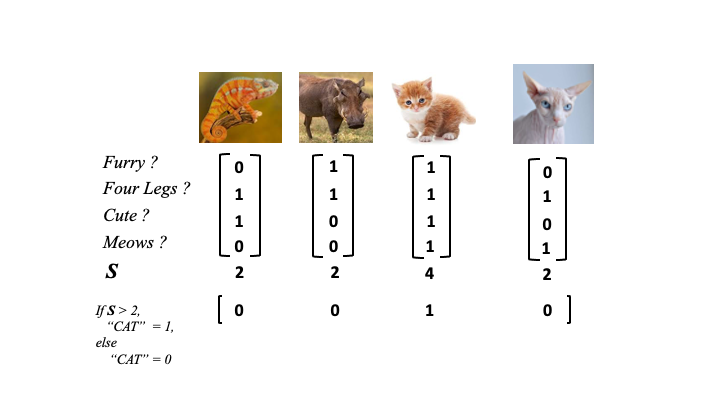
\includegraphics{figs/percepwts/Slide3.png}

Only one of the actual cats was correctly labelled. The clever part of the neural network is to apply weights to each of the features that modify the value they add to the neural network (in the figure below as blue values).

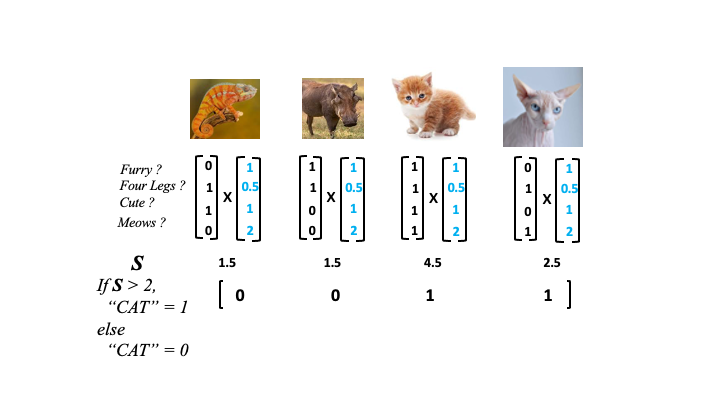
\includegraphics{figs/percepwts/Slide4.png}

Weights work to give the more useful features higher values (like \texttt{meows}) and less useful features lower values (like \texttt{four\ legs}). The network can now more accurately classify the animals in the picture.

\hypertarget{neural-network-structure}{%
\subsection{Neural Network Structure}\label{neural-network-structure}}

The networks needn't be restricted to simple structures in which the initial inputs go straight to the output, many layers of neurons can be made, each arbitrary numbers of neurons deep. These extra layers are called the hidden layers

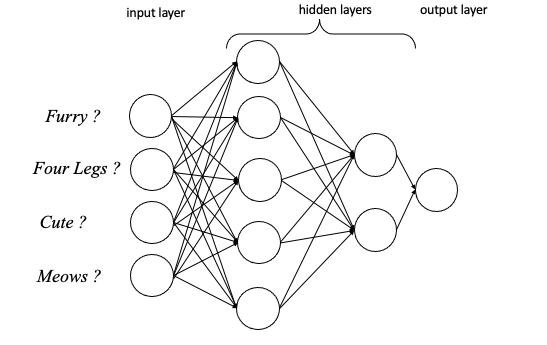
\includegraphics{figs/layers.png}

The hidden layers increase the power of the neural network by allowing for further integration of information and extra weighting. But they also make the network more obscure and hard to read, again this is how the power of the neural network comes at the expense of interpretability.

\hypertarget{training-to-find-weights}{%
\subsection{Training to find weights}\label{training-to-find-weights}}

The main part of training the neural network and the place it makes itself powerful is in the weight finding phase. This is called the learning or training phase. To do this the training algorithm goes back and forth across the network methodically adjusting the weights until it sees no further improvement when classifying on the training data - it is constantly comparing its current state against the answers in the training data.

\hypertarget{neural-network-training-phases-are-long-and-involved}{%
\subsection{Neural network training phases are long and involved}\label{neural-network-training-phases-are-long-and-involved}}

As you can see there is a lot about neural networks to be specified and optimised. The number and depth of hidden layers that is optimal varies for each data set and there is no rule to follow as to what will be best. It is also not true that bigger is always better. The weights of the neural network must also be optimised for every data set, and we must be careful to use training data that is distinct from our test data to be confident in the generality of our resulting model. As a result of these considerations the training and testing phases of neural networks are particularly involved.

We won't go through that whole procedure here, though you should be aware of it as it is the key to a truly useful deep learning model. But we will try out a small neural network in R.

\hypertarget{a-simple-neural-network-in-r}{%
\section{A simple neural network in R}\label{a-simple-neural-network-in-r}}

\hypertarget{frog-data}{%
\subsection{Frog Data}\label{frog-data}}

In this example we shall use some data on amphibian presence at various sites. Here's a \texttt{glimpse()} of the \texttt{train\_rows}, we also have a \texttt{test\_rows}

\begin{Shaded}
\begin{Highlighting}[]
\NormalTok{dplyr}\OperatorTok{::}\KeywordTok{glimpse}\NormalTok{(train_rows)}
\end{Highlighting}
\end{Shaded}

\begin{verbatim}
## Rows: 94
## Columns: 20
## $ SR                 <dbl> 1000, 100, 200, 30000, 10050, 700, 50, 8000, 2500, ~
## $ NR                 <dbl> 1, 1, 1, 1, 1, 1, 1, 1, 1, 1, 4, 1, 1, 2, 1, 1, 1, ~
## $ TR                 <dbl> 1, 1, 5, 1, 1, 5, 1, 1, 1, 2, 1, 1, 1, 1, 14, 1, 14~
## $ VR                 <dbl> 3, 2, 1, 3, 2, 2, 2, 3, 3, 0, 1, 2, 3, 2, 3, 3, 1, ~
## $ SUR1               <dbl> 2, 2, 10, 1, 1, 10, 2, 2, 10, 6, 2, 2, 2, 2, 7, 2, ~
## $ SUR2               <dbl> 1, 7, 6, 1, 10, 6, 7, 10, 2, 9, 7, 7, 2, 10, 2, 2, ~
## $ SUR3               <dbl> 9, 6, 10, 1, 6, 9, 10, 7, 6, 2, 6, 9, 1, 10, 1, 7, ~
## $ UR                 <dbl> 0, 0, 3, 0, 0, 0, 0, 0, 0, 0, 3, 0, 1, 0, 0, 0, 0, ~
## $ FR                 <dbl> 0, 0, 4, 0, 1, 0, 0, 0, 1, 0, 2, 0, 0, 0, 0, 0, 0, ~
## $ OR                 <dbl> 100, 100, 75, 100, 100, 100, 100, 100, 100, 50, 100~
## $ RR                 <dbl> 2, 2, 1, 2, 5, 1, 5, 9, 0, 0, 0, 0, 5, 1, 5, 0, 5, ~
## $ BR                 <dbl> 5, 2, 1, 10, 5, 1, 5, 9, 1, 0, 0, 0, 5, 5, 5, 1, 5,~
## $ MR                 <dbl> 0, 2, 0, 0, 0, 0, 0, 0, 0, 0, 0, 0, 0, 0, 0, 0, 0, ~
## $ CR                 <dbl> 1, 1, 1, 1, 1, 1, 1, 1, 1, 1, 1, 1, 1, 1, 1, 1, 1, ~
## $ Green_frogs        <dbl> 0, 1, 0, 1, 0, 1, 1, 0, 1, 1, 1, 0, 1, 0, 1, 0, 0, ~
## $ Brown_frogs        <dbl> 0, 0, 1, 1, 1, 1, 1, 1, 0, 1, 1, 0, 1, 1, 1, 1, 1, ~
## $ Common_toad        <dbl> 0, 0, 1, 1, 1, 0, 1, 1, 1, 1, 1, 1, 1, 0, 1, 1, 1, ~
## $ Tree_frog          <dbl> 1, 0, 0, 1, 0, 0, 0, 0, 0, 0, 0, 0, 0, 0, 1, 1, 1, ~
## $ Common_newt        <dbl> 0, 0, 1, 0, 1, 0, 0, 0, 1, 0, 0, 0, 1, 0, 1, 0, 0, ~
## $ Great_crested_newt <dbl> 0, 0, 0, 0, 1, 0, 0, 0, 0, 0, 0, 0, 1, 0, 0, 0, 0, ~
\end{verbatim}

These data are from \citep{frogs} originally and you can see a description of the 20 columns at \url{https://archive.ics.uci.edu/ml/datasets/Amphibians}. Briefly, they are things like the presence and size and maintenance of reservoirs and the surrounding area, whether humans use the area, whether there is fishing. All potentially pertinent measurements. The presence of different types of amphibian species are recorded as 1 for present, and 0 for not present.

We could use a neural network to predict any of the species listed, but let's work on predicting \texttt{Green\_frogs}.

We'll use the straightforward \texttt{neuralnet()} function in the \texttt{neuralnet} package for this. It can take an R formula specification, which as you'll recall takes the form \texttt{y\ \textasciitilde{}\ feature\_1\ +\ feature\_2\ ...} where \texttt{y} is the thing to be predicted and \texttt{feature\_x} are the features to input for prediction with. With 19 to enter, that's lots of typing, so I've squashed it into a variable called \texttt{long\_formula}

\begin{Shaded}
\begin{Highlighting}[]
\NormalTok{long_formula}
\end{Highlighting}
\end{Shaded}

\begin{verbatim}
## Green_frogs ~ SR + NR + TR + VR + SUR1 + SUR2 + SUR3 + UR + FR + 
##     OR + RR + BR + MR + CR + Green_frogs + Brown_frogs + Common_toad + 
##     Tree_frog + Common_newt + Great_crested_newt
\end{verbatim}

\hypertarget{training-a-3-hidden-layer-neural-network}{%
\subsection{Training a 3 hidden layer neural network}\label{training-a-3-hidden-layer-neural-network}}

We can put the formula into the function \texttt{neuralnet()} specify the training data and the depth of the hidden layers. Here we'll have 3, with 15, 10 and 5 neurons respectively.

\begin{Shaded}
\begin{Highlighting}[]
\KeywordTok{library}\NormalTok{(neuralnet)}
\end{Highlighting}
\end{Shaded}

\begin{verbatim}
## 
## Attaching package: 'neuralnet'
\end{verbatim}

\begin{verbatim}
## The following object is masked from 'package:dplyr':
## 
##     compute
\end{verbatim}

\begin{Shaded}
\begin{Highlighting}[]
\NormalTok{nn <-}\StringTok{ }\KeywordTok{neuralnet}\NormalTok{(long_formula, train_rows, }\DataTypeTok{hidden=}\KeywordTok{c}\NormalTok{(}\DecValTok{15}\NormalTok{,}\DecValTok{10}\NormalTok{,}\DecValTok{5}\NormalTok{), }\DataTypeTok{linear.output=}\OtherTok{FALSE}\NormalTok{)}
\end{Highlighting}
\end{Shaded}

That single step builds the neural network, and trains it and gives it back to use so we can use it to make predictions with. Of course the first thing we want to make predictions on is our test set so we can evaluate the accuracy.

\hypertarget{testing-the-neural-network}{%
\subsection{Testing the neural network}\label{testing-the-neural-network}}

The \texttt{compute()} function takes a neural network model and data and creates predictions. Here we feed it our test data. However when we look at the resulting predictions (stored in the \texttt{net.result} slot in our \texttt{predictions} object) we see something odd.

\begin{Shaded}
\begin{Highlighting}[]
\NormalTok{predictions <-}\StringTok{ }\KeywordTok{compute}\NormalTok{(nn, test_rows)}
\KeywordTok{head}\NormalTok{(predictions}\OperatorTok{$}\NormalTok{net.result)}
\end{Highlighting}
\end{Shaded}

\begin{verbatim}
##             [,1]
## [1,] 0.998154554
## [2,] 0.998147802
## [3,] 0.008503821
## [4,] 0.998154554
## [5,] 0.996971835
## [6,] 0.006267082
\end{verbatim}

The predictions are not of classes, but are actually numbers that represent the level of sureness the model has that the site has Green Frogs. This value is sometimes useful, but we need to convert it to classes to evaluate it. As the values run between 0 and 1 we can do that by simple rounding so that any prediction over 0.5 is considered a present prediction, anything below is consider an absent predictions (other algorithms and functions exist for this conversion).

\begin{Shaded}
\begin{Highlighting}[]
\NormalTok{binary_predictions <-}\StringTok{ }\KeywordTok{round}\NormalTok{(predictions}\OperatorTok{$}\NormalTok{net.result,}\DataTypeTok{digits=}\DecValTok{0}\NormalTok{)}
\end{Highlighting}
\end{Shaded}

We can then put those binarised predictions into the \texttt{confusionMatrix()} function we used previously alongside the true values from the \texttt{test\_rows} data (remembering to convert them to \texttt{factors} as they are not already).

\begin{Shaded}
\begin{Highlighting}[]
\KeywordTok{library}\NormalTok{(caret)}
\KeywordTok{confusionMatrix}\NormalTok{(}\KeywordTok{factor}\NormalTok{(test_rows}\OperatorTok{$}\NormalTok{Green_frogs), }\KeywordTok{factor}\NormalTok{(binary_predictions))}
\end{Highlighting}
\end{Shaded}

\begin{verbatim}
## Confusion Matrix and Statistics
## 
##           Reference
## Prediction  0  1
##          0 30  4
##          1 19 42
##                                           
##                Accuracy : 0.7579          
##                  95% CI : (0.6592, 0.8399)
##     No Information Rate : 0.5158          
##     P-Value [Acc > NIR] : 1.097e-06       
##                                           
##                   Kappa : 0.5201          
##                                           
##  Mcnemar's Test P-Value : 0.003509        
##                                           
##             Sensitivity : 0.6122          
##             Specificity : 0.9130          
##          Pos Pred Value : 0.8824          
##          Neg Pred Value : 0.6885          
##              Prevalence : 0.5158          
##          Detection Rate : 0.3158          
##    Detection Prevalence : 0.3579          
##       Balanced Accuracy : 0.7626          
##                                           
##        'Positive' Class : 0               
## 
\end{verbatim}

We can see the resulting network has about 60\% sensitivity and 90\% specificity, so missing a lot of real green frog sites.

As you can imagine the exact choice of the parameters can make a difference on final neural network performance. This is just one instance. In real analyses we would try out many different hidden layer and other parameter configurations and select the best performing at the the testing stage. That may then even move on to a further fine tuning stage, the development of machine learners is art as much as it is science.

\hypertarget{examining-the-structure-of-the-neural-network}{%
\subsection{Examining the structure of the neural network}\label{examining-the-structure-of-the-neural-network}}

The \texttt{neuralnet} package we used here was chosen not least because it is straightforward and fast, but also because it is possible to get a plot of the created network.

\begin{Shaded}
\begin{Highlighting}[]
\KeywordTok{plot}\NormalTok{(nn)}
\end{Highlighting}
\end{Shaded}

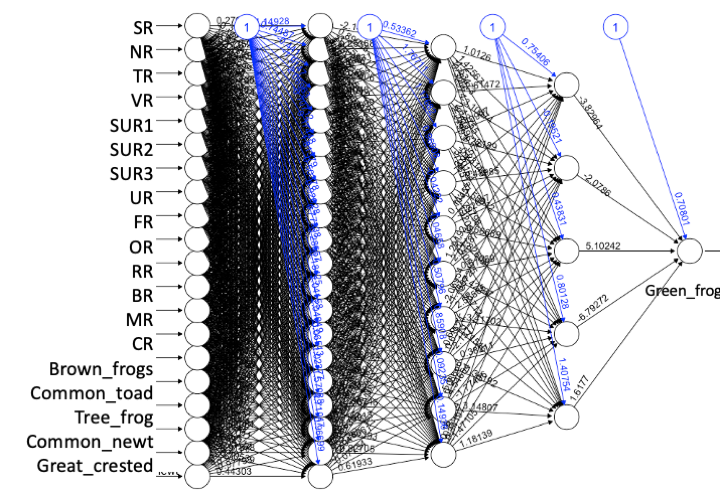
\includegraphics{figs/nn_viz.png}

Note that the first layer corresponds to the input columns in the data with one neuron each, these then feed into the 3 hidden layers we specified of 20,15 and 5 layers each and finally the one neuron layer intergrating everything to give us the final prediction on whether we have a Green Frog.

We can see that the neural network we made is really complex. Even with just the small number of input features and hidden layers we have the combinations of weights and their effect into the next layer is too hard to understand (even if the plot were readable). This shows us how neural network structures become black boxes, we can't be sure which of the input variables (or combinations of which) were most important in making the classifications.

\begin{roundup}
\begin{itemize}
\tightlist
\item
  Deep Learners choose their own features
\item
  Deep Learners like neural networks can work on patterns we dont explicitly state
\item
  Neural network training means finding weights that give the best classifications
\item
  Neural networks are black boxes and hard to interpret
\end{itemize}
\end{roundup}

  \bibliography{book.bib,packages.bib}

\end{document}
